\documentclass[twoside]{book}

% Packages required by doxygen
\usepackage{fixltx2e}
\usepackage{calc}
\usepackage{doxygen}
\usepackage[export]{adjustbox} % also loads graphicx
\usepackage{graphicx}
\usepackage[utf8]{inputenc}
\usepackage{makeidx}
\usepackage{multicol}
\usepackage{multirow}
\PassOptionsToPackage{warn}{textcomp}
\usepackage{textcomp}
\usepackage[nointegrals]{wasysym}
\usepackage[table]{xcolor}

% Font selection
\usepackage[T1]{fontenc}
\usepackage[scaled=.90]{helvet}
\usepackage{courier}
\usepackage{amssymb}
\usepackage{sectsty}
\renewcommand{\familydefault}{\sfdefault}
\allsectionsfont{%
  \fontseries{bc}\selectfont%
  \color{darkgray}%
}
\renewcommand{\DoxyLabelFont}{%
  \fontseries{bc}\selectfont%
  \color{darkgray}%
}
\newcommand{\+}{\discretionary{\mbox{\scriptsize$\hookleftarrow$}}{}{}}

% Page & text layout
\usepackage{geometry}
\geometry{%
  a4paper,%
  top=2.5cm,%
  bottom=2.5cm,%
  left=2.5cm,%
  right=2.5cm%
}
\tolerance=750
\hfuzz=15pt
\hbadness=750
\setlength{\emergencystretch}{15pt}
\setlength{\parindent}{0cm}
\setlength{\parskip}{0.2cm}
\makeatletter
\renewcommand{\paragraph}{%
  \@startsection{paragraph}{4}{0ex}{-1.0ex}{1.0ex}{%
    \normalfont\normalsize\bfseries\SS@parafont%
  }%
}
\renewcommand{\subparagraph}{%
  \@startsection{subparagraph}{5}{0ex}{-1.0ex}{1.0ex}{%
    \normalfont\normalsize\bfseries\SS@subparafont%
  }%
}
\makeatother

% Headers & footers
\usepackage{fancyhdr}
\pagestyle{fancyplain}
\fancyhead[LE]{\fancyplain{}{\bfseries\thepage}}
\fancyhead[CE]{\fancyplain{}{}}
\fancyhead[RE]{\fancyplain{}{\bfseries\leftmark}}
\fancyhead[LO]{\fancyplain{}{\bfseries\rightmark}}
\fancyhead[CO]{\fancyplain{}{}}
\fancyhead[RO]{\fancyplain{}{\bfseries\thepage}}
\fancyfoot[LE]{\fancyplain{}{}}
\fancyfoot[CE]{\fancyplain{}{}}
\fancyfoot[RE]{\fancyplain{}{\bfseries\scriptsize Generated on Fri Jul 17 2015 17\+:52\+:21 for Bridges-\/\+C++-\/2.\+0 by Doxygen }}
\fancyfoot[LO]{\fancyplain{}{\bfseries\scriptsize Generated on Fri Jul 17 2015 17\+:52\+:21 for Bridges-\/\+C++-\/2.\+0 by Doxygen }}
\fancyfoot[CO]{\fancyplain{}{}}
\fancyfoot[RO]{\fancyplain{}{}}
\renewcommand{\footrulewidth}{0.4pt}
\renewcommand{\chaptermark}[1]{%
  \markboth{#1}{}%
}
\renewcommand{\sectionmark}[1]{%
  \markright{\thesection\ #1}%
}

% Indices & bibliography
\usepackage{natbib}
\usepackage[titles]{tocloft}
\setcounter{tocdepth}{3}
\setcounter{secnumdepth}{5}
\makeindex

% Hyperlinks (required, but should be loaded last)
\usepackage{ifpdf}
\ifpdf
  \usepackage[pdftex,pagebackref=true]{hyperref}
\else
  \usepackage[ps2pdf,pagebackref=true]{hyperref}
\fi
\hypersetup{%
  colorlinks=true,%
  linkcolor=blue,%
  citecolor=blue,%
  unicode%
}

% Custom commands
\newcommand{\clearemptydoublepage}{%
  \newpage{\pagestyle{empty}\cleardoublepage}%
}


%===== C O N T E N T S =====

\begin{document}

% Titlepage & ToC
\hypersetup{pageanchor=false,
             bookmarks=true,
             bookmarksnumbered=true,
             pdfencoding=unicode
            }
\pagenumbering{roman}
\begin{titlepage}
\vspace*{7cm}
\begin{center}%
{\Large Bridges-\/\+C++-\/2.0 \\[1ex]\large 2.\+0.\+0 }\\
\vspace*{1cm}
{\large Generated by Doxygen 1.8.9.1}\\
\vspace*{0.5cm}
{\small Fri Jul 17 2015 17:52:21}\\
\end{center}
\end{titlepage}
\clearemptydoublepage
\tableofcontents
\clearemptydoublepage
\pagenumbering{arabic}
\hypersetup{pageanchor=true}

%--- Begin generated contents ---
\chapter{Namespace Index}
\section{Namespace List}
Here is a list of all namespaces with brief descriptions\+:\begin{DoxyCompactList}
\item\contentsline{section}{\hyperlink{namespacebridges}{bridges} }{\pageref{namespacebridges}}{}
\end{DoxyCompactList}

\chapter{Hierarchical Index}
\section{Class Hierarchy}
This inheritance list is sorted roughly, but not completely, alphabetically\+:\begin{DoxyCompactList}
\item \contentsline{section}{bridges\+:\+:A\+D\+T\+Visualizer$<$ K, E $>$}{\pageref{classbridges_1_1_a_d_t_visualizer}}{}
\item \contentsline{section}{bridges\+:\+:Bridges$<$ K, E $>$}{\pageref{classbridges_1_1_bridges}}{}
\item \contentsline{section}{bridges\+:\+:Connector}{\pageref{classbridges_1_1_connector}}{}
\item \contentsline{section}{bridges\+:\+:Edge$<$ Key $>$}{\pageref{classbridges_1_1_edge}}{}
\item \contentsline{section}{bridges\+:\+:Element$<$ E $>$}{\pageref{classbridges_1_1_element}}{}
\begin{DoxyCompactList}
\item \contentsline{section}{bridges\+:\+:D\+Lelement$<$ E $>$}{\pageref{classbridges_1_1_d_lelement}}{}
\item \contentsline{section}{bridges\+:\+:S\+Lelement$<$ E $>$}{\pageref{classbridges_1_1_s_lelement}}{}
\item \contentsline{section}{bridges\+:\+:Tree\+Element$<$ E $>$}{\pageref{classbridges_1_1_tree_element}}{}
\begin{DoxyCompactList}
\item \contentsline{section}{bridges\+:\+:B\+S\+T\+Element$<$ K, E $>$}{\pageref{classbridges_1_1_b_s_t_element}}{}
\end{DoxyCompactList}
\end{DoxyCompactList}
\item \contentsline{section}{bridges\+:\+:Element$<$ bridges\+:\+:Edge$<$ Key $>$ $>$}{\pageref{classbridges_1_1_element}}{}
\begin{DoxyCompactList}
\item \contentsline{section}{bridges\+:\+:S\+Lelement$<$ bridges\+:\+:Edge$<$ Key $>$ $>$}{\pageref{classbridges_1_1_s_lelement}}{}
\end{DoxyCompactList}
\item \contentsline{section}{bridges\+:\+:Element\+Visualizer}{\pageref{classbridges_1_1_element_visualizer}}{}
\item \contentsline{section}{bridges\+:\+:Graph\+Adj\+List$<$ Key, E $>$}{\pageref{classbridges_1_1_graph_adj_list}}{}
\item \contentsline{section}{bridges\+:\+:Graph\+Adj\+List$<$ K, E $>$}{\pageref{classbridges_1_1_graph_adj_list}}{}
\item \contentsline{section}{bridges\+:\+:Graph\+Adj\+Matrix$<$ Key, E $>$}{\pageref{classbridges_1_1_graph_adj_matrix}}{}
\item \contentsline{section}{bridges\+:\+:Graph\+Adj\+Matrix$<$ K, E $>$}{\pageref{classbridges_1_1_graph_adj_matrix}}{}
\item \contentsline{section}{bridges\+:\+:Link\+Visualizer}{\pageref{classbridges_1_1_link_visualizer}}{}
\item \contentsline{section}{bridges\+:\+:Validation}{\pageref{classbridges_1_1_validation}}{}
\end{DoxyCompactList}

\chapter{Class Index}
\section{Class List}
Here are the classes, structs, unions and interfaces with brief descriptions\+:\begin{DoxyCompactList}
\item\contentsline{section}{\hyperlink{classbridges_1_1_a_d_t_visualizer}{bridges\+::\+A\+D\+T\+Visualizer$<$ K, E $>$} }{\pageref{classbridges_1_1_a_d_t_visualizer}}{}
\item\contentsline{section}{\hyperlink{classbridges_1_1_bridges}{bridges\+::\+Bridges$<$ K, E $>$} }{\pageref{classbridges_1_1_bridges}}{}
\item\contentsline{section}{\hyperlink{classbridges_1_1_b_s_t_element}{bridges\+::\+B\+S\+T\+Element$<$ K, E $>$} }{\pageref{classbridges_1_1_b_s_t_element}}{}
\item\contentsline{section}{\hyperlink{classbridges_1_1_connector}{bridges\+::\+Connector} }{\pageref{classbridges_1_1_connector}}{}
\item\contentsline{section}{\hyperlink{classbridges_1_1_d_lelement}{bridges\+::\+D\+Lelement$<$ E $>$} }{\pageref{classbridges_1_1_d_lelement}}{}
\item\contentsline{section}{\hyperlink{classbridges_1_1_edge}{bridges\+::\+Edge$<$ Key $>$} }{\pageref{classbridges_1_1_edge}}{}
\item\contentsline{section}{\hyperlink{classbridges_1_1_element}{bridges\+::\+Element$<$ E $>$} }{\pageref{classbridges_1_1_element}}{}
\item\contentsline{section}{\hyperlink{classbridges_1_1_element_visualizer}{bridges\+::\+Element\+Visualizer} }{\pageref{classbridges_1_1_element_visualizer}}{}
\item\contentsline{section}{\hyperlink{classbridges_1_1_graph_adj_list}{bridges\+::\+Graph\+Adj\+List$<$ Key, E $>$} }{\pageref{classbridges_1_1_graph_adj_list}}{}
\item\contentsline{section}{\hyperlink{classbridges_1_1_graph_adj_matrix}{bridges\+::\+Graph\+Adj\+Matrix$<$ Key, E $>$} }{\pageref{classbridges_1_1_graph_adj_matrix}}{}
\item\contentsline{section}{\hyperlink{classbridges_1_1_link_visualizer}{bridges\+::\+Link\+Visualizer} }{\pageref{classbridges_1_1_link_visualizer}}{}
\item\contentsline{section}{\hyperlink{classbridges_1_1_s_lelement}{bridges\+::\+S\+Lelement$<$ E $>$} }{\pageref{classbridges_1_1_s_lelement}}{}
\item\contentsline{section}{\hyperlink{classbridges_1_1_tree_element}{bridges\+::\+Tree\+Element$<$ E $>$} }{\pageref{classbridges_1_1_tree_element}}{}
\item\contentsline{section}{\hyperlink{classbridges_1_1_validation}{bridges\+::\+Validation} }{\pageref{classbridges_1_1_validation}}{}
\end{DoxyCompactList}

\chapter{File Index}
\section{File List}
Here is a list of all files with brief descriptions\+:\begin{DoxyCompactList}
\item\contentsline{section}{src/\hyperlink{_a_d_t_visualizer_8h}{A\+D\+T\+Visualizer.\+h} }{\pageref{_a_d_t_visualizer_8h}}{}
\item\contentsline{section}{src/\hyperlink{_array_8h}{Array.\+h} }{\pageref{_array_8h}}{}
\item\contentsline{section}{src/\hyperlink{_bridges_8h}{Bridges.\+h} }{\pageref{_bridges_8h}}{}
\item\contentsline{section}{src/\hyperlink{_b_s_t_element_8h}{B\+S\+T\+Element.\+h} }{\pageref{_b_s_t_element_8h}}{}
\item\contentsline{section}{src/\hyperlink{_connector_8h}{Connector.\+h} }{\pageref{_connector_8h}}{}
\item\contentsline{section}{src/\hyperlink{_d_lelement_8h}{D\+Lelement.\+h} }{\pageref{_d_lelement_8h}}{}
\item\contentsline{section}{src/\hyperlink{_edge_8h}{Edge.\+h} }{\pageref{_edge_8h}}{}
\item\contentsline{section}{src/\hyperlink{_element_8h}{Element.\+h} }{\pageref{_element_8h}}{}
\item\contentsline{section}{src/\hyperlink{_element_visualizer_8h}{Element\+Visualizer.\+h} }{\pageref{_element_visualizer_8h}}{}
\item\contentsline{section}{src/\hyperlink{_graph_adj_list_8h}{Graph\+Adj\+List.\+h} }{\pageref{_graph_adj_list_8h}}{}
\item\contentsline{section}{src/\hyperlink{_graph_adj_matrix_8h}{Graph\+Adj\+Matrix.\+h} }{\pageref{_graph_adj_matrix_8h}}{}
\item\contentsline{section}{src/\hyperlink{_link_visualizer_8h}{Link\+Visualizer.\+h} }{\pageref{_link_visualizer_8h}}{}
\item\contentsline{section}{src/\hyperlink{_s_lelement_8h}{S\+Lelement.\+h} }{\pageref{_s_lelement_8h}}{}
\item\contentsline{section}{src/\hyperlink{_tree_element_8h}{Tree\+Element.\+h} }{\pageref{_tree_element_8h}}{}
\item\contentsline{section}{src/\hyperlink{_validation_8h}{Validation.\+h} }{\pageref{_validation_8h}}{}
\end{DoxyCompactList}

\chapter{Namespace Documentation}
\hypertarget{namespacebridges}{}\section{bridges Namespace Reference}
\label{namespacebridges}\index{bridges@{bridges}}
\subsection*{Classes}
\begin{DoxyCompactItemize}
\item 
class \hyperlink{classbridges_1_1_a_d_t_visualizer}{A\+D\+T\+Visualizer}
\item 
class \hyperlink{classbridges_1_1_bridges}{Bridges}
\item 
class \hyperlink{classbridges_1_1_b_s_t_element}{B\+S\+T\+Element}
\item 
class \hyperlink{classbridges_1_1_connector}{Connector}
\item 
class \hyperlink{classbridges_1_1_d_lelement}{D\+Lelement}
\item 
class \hyperlink{classbridges_1_1_edge}{Edge}
\item 
class \hyperlink{classbridges_1_1_element}{Element}
\item 
class \hyperlink{classbridges_1_1_element_visualizer}{Element\+Visualizer}
\item 
class \hyperlink{classbridges_1_1_graph_adj_list}{Graph\+Adj\+List}
\item 
class \hyperlink{classbridges_1_1_graph_adj_matrix}{Graph\+Adj\+Matrix}
\item 
class \hyperlink{classbridges_1_1_link_visualizer}{Link\+Visualizer}
\item 
class \hyperlink{classbridges_1_1_s_lelement}{S\+Lelement}
\item 
class \hyperlink{classbridges_1_1_tree_element}{Tree\+Element}
\item 
class \hyperlink{classbridges_1_1_validation}{Validation}
\end{DoxyCompactItemize}


\subsection{Detailed Description}
The \hyperlink{classbridges_1_1_a_d_t_visualizer}{A\+D\+T\+Visualizer} class is responsible for taking a data structure as input and generating a J\+S\+O\+N representation prior to sending it to the server for visualization. The \hyperlink{classbridges_1_1_bridges}{Bridges} class uses this object to keep track of the Visualization representation. 

An end user will generally not need to interact directly with this class.

\begin{DoxyAuthor}{Author}
Kalpathi Subramanian (C++ port), 6/15/15
\end{DoxyAuthor}
Connection to the \hyperlink{classbridges_1_1_bridges}{Bridges} server.

This class contains the needed initialization functions for B\+R\+I\+D\+G\+E\+S and the needed infrastructure to connect to the server

\begin{DoxyAuthor}{Author}
Kalpathi Subramanian (C++ port)
\end{DoxyAuthor}

\begin{DoxyParams}{Parameters}
{\em Generic} & parameters $<$K, E$>$, K is any orderable type (short, unsigned, int, float, double, char, string), E is any legal type that represents application data.\\
\hline
\end{DoxyParams}
This class can be used to create doubly linked element objects with next and previous (prev) pointers

\begin{DoxyAuthor}{Author}
Kalpathi Subramanian, 6/11/15
\end{DoxyAuthor}
This class is used to assign a visual connection between two Elements in the \hyperlink{classbridges_1_1_bridges}{Bridges} Visualization. 

\hyperlink{classbridges_1_1_bridges}{Bridges} will represent these as arrows between two Elements. The starting \hyperlink{classbridges_1_1_element}{Element} of the arrow will be referred to as the source \hyperlink{classbridges_1_1_element}{Element} and the ending \hyperlink{classbridges_1_1_element}{Element} of the arrow will be referred to as the terminating \hyperlink{classbridges_1_1_element}{Element}.

\begin{DoxyAuthor}{Author}
krs
\end{DoxyAuthor}

\begin{DoxyParams}{Parameters}
{\em $<$\+E$>$} & This is the Superclass \hyperlink{classbridges_1_1_element}{Element} with \hyperlink{classbridges_1_1_s_lelement}{S\+Lelement}, \hyperlink{classbridges_1_1_d_lelement}{D\+Lelement}, Array\+List\+Element, \hyperlink{classbridges_1_1_tree_element}{Tree\+Element}, \hyperlink{classbridges_1_1_b_s_t_element}{B\+S\+T\+Element} subclasses. Generic parameter E is provided and all application specific data can be stored here). An object of E data type can be integer, string, Tweet, Actor, Movie, Earthquake\+Tweet, etc. The label field(string type) is used to label the visualization of the element node. \hyperlink{classbridges_1_1_element}{Element} has two visualizer objects. \hyperlink{classbridges_1_1_element_visualizer}{Element\+Visualizer} holds properties of the element itself, and \hyperlink{classbridges_1_1_link_visualizer}{Link\+Visualizer}, which holds properties of the link between this element and the element it is linked to -- useful in linked structures and graphs that contain edges. Identifier field automatically generated\\
\hline
\end{DoxyParams}
\begin{DoxyAuthor}{Author}
Kalpathi Subramanian, 6/11/15
\end{DoxyAuthor}
This class is used to store the visualization elements on the for the \hyperlink{classbridges_1_1_bridges}{Bridges} Visualiztion, including the color, shape, opacity, and size of the node. 

Objects of this class are stored as properties of all \hyperlink{classbridges_1_1_element}{Element} subclasses. Generally, you will manipulating the \hyperlink{classbridges_1_1_element_visualizer}{Element\+Visualizer} returned from the \hyperlink{classbridges_1_1_element}{Element} get\+Visualizer() method, and then call the set\+Visualizer() method on the \hyperlink{classbridges_1_1_element}{Element} after changes have been made.

The \hyperlink{classbridges_1_1_graph_adj_list}{Graph\+Adj\+List} class can be used to represent adjacency list based graphs in B\+R\+I\+D\+G\+Es, with E represnting a data specific generic parameter. The class is simply a wrapper around the C++ S\+T\+L unordered\+\_\+map class and, thus, derives all its operations from it. B\+R\+I\+D\+G\+E\+S provides methods to visualize the graph and its contents.

Author\+: Kalpathi Subramanian, 6/29/15


\begin{DoxyParams}{Parameters}
{\em Element$<$\+E$>$} & This class is used to keep the visual properties of links that art of data structures such as linked lists, pointer based trees, link based graph representations, etc. Relevant attributes include color, thickness, opacity, line end point attributes. \\
\hline
\end{DoxyParams}
Objects of this class are stored as properties of all \hyperlink{classbridges_1_1_element}{Element} subclasses. Generally, you will manipulating the \hyperlink{classbridges_1_1_link_visualizer}{Link\+Visualizer} returned from the \hyperlink{classbridges_1_1_element}{Element} get\+Link\+Visualizer() method, and then call the set\+Link\+Visualizer() method on the \hyperlink{classbridges_1_1_element}{Element} after changes have been made.

This class can be used to instantiate Singly List Elements with identifiers (automatically generated), labels (derived from the values of E or manually set) next pointers an object of E data type\+: integer, string, Tweet, Actor, Movie, Earthquake\+Tweet, etc. element visualizer objects containing all the C\+S\+S atributes (color, shape, opacity, size) necessary for displaying them in a web browser \begin{DoxyAuthor}{Author}
Kalpathi Subramanian, 6/11/15.
\end{DoxyAuthor}

\begin{DoxyParams}{Parameters}
{\em $<$\+E$>$} & \\
\hline
\end{DoxyParams}
\begin{DoxyAuthor}{Author}
Kalpathi Subramanian, 6/12/15 This class can be used to create tree element objects with left and right pointers 
\end{DoxyAuthor}

\chapter{Class Documentation}
\hypertarget{classbridges_1_1_a_d_t_visualizer}{}\section{bridges\+:\+:A\+D\+T\+Visualizer$<$ K, E $>$ Class Template Reference}
\label{classbridges_1_1_a_d_t_visualizer}\index{bridges\+::\+A\+D\+T\+Visualizer$<$ K, E $>$@{bridges\+::\+A\+D\+T\+Visualizer$<$ K, E $>$}}


{\ttfamily \#include $<$A\+D\+T\+Visualizer.\+h$>$}

\subsection*{Public Member Functions}
\begin{DoxyCompactItemize}
\item 
\hyperlink{classbridges_1_1_a_d_t_visualizer_a7aeb662bedb4275ae3b4d9e6042771ea}{A\+D\+T\+Visualizer} ()
\item 
bool \hyperlink{classbridges_1_1_a_d_t_visualizer_a5705e913cd68b365dbcce735b244fc19}{is\+Visualize\+J\+S\+O\+N} ()
\item 
void \hyperlink{classbridges_1_1_a_d_t_visualizer_a3df170e02b0e64324b02987823a7d39d}{set\+Visualize\+J\+S\+O\+N} (bool vis\+\_\+json\+\_\+flag)
\item 
string \hyperlink{classbridges_1_1_a_d_t_visualizer_a8341eff2cb8069224671f5c7e99ebc27}{get\+Visualizer\+Identifier} ()
\item 
void \hyperlink{classbridges_1_1_a_d_t_visualizer_aa8744e8d1d2b308134a143489a1d99bf}{set\+Visualizer\+Identifier} (string vis\+\_\+identifier)
\item 
string \hyperlink{classbridges_1_1_a_d_t_visualizer_af64c11473910177160374c7ab10088ee}{get\+Visualizer\+Type} ()
\item 
void \hyperlink{classbridges_1_1_a_d_t_visualizer_a729ef76a688915b6e3e076c2311d9bef}{set\+Array\+Size} (int size)
\item 
int \hyperlink{classbridges_1_1_a_d_t_visualizer_a2a88784e70202d2f782e9bfe5570ed54}{get\+Array\+Size} ()
\item 
void \hyperlink{classbridges_1_1_a_d_t_visualizer_a6ab87acd793e9db9d2769f3fc36f38ee}{set\+Visualizer\+Type} (string vis\+\_\+type)
\item 
string \hyperlink{classbridges_1_1_a_d_t_visualizer_a804d83b3b21c18df6b12f7b9ca493a36}{get\+Data\+Structure\+Representation} (\hyperlink{classbridges_1_1_graph_adj_matrix}{Graph\+Adj\+Matrix}$<$ K, E $>$ $\ast$graph\+\_\+adj\+\_\+matrix)
\item 
string \hyperlink{classbridges_1_1_a_d_t_visualizer_ac644b78b92ce163545806fe5e43c2eb0}{get\+Data\+Structure\+Representation} (\hyperlink{classbridges_1_1_graph_adj_list}{Graph\+Adj\+List}$<$ K, E $>$ $\ast$graph\+\_\+adj\+\_\+list)
\item 
string \hyperlink{classbridges_1_1_a_d_t_visualizer_ab6e6c797e4ec549a5bbf16fd156070e1}{get\+Data\+Structure\+Representation} (\hyperlink{classbridges_1_1_s_lelement}{S\+Lelement}$<$ E $>$ $\ast$first\+\_\+element)
\item 
string \hyperlink{classbridges_1_1_a_d_t_visualizer_ade7d2f57dc4cd2668f7029ace748f5cf}{get\+Data\+Structure\+Representation} (\hyperlink{classbridges_1_1_d_lelement}{D\+Lelement}$<$ E $>$ $\ast$first\+\_\+element)
\item 
string \hyperlink{classbridges_1_1_a_d_t_visualizer_a14b4c76bc8d4ea378faec291761b078a}{get\+Data\+Structure\+Representation} (\hyperlink{classbridges_1_1_element}{Element}$<$ E $>$ $\ast$b\+\_\+array)
\item 
string \hyperlink{classbridges_1_1_a_d_t_visualizer_a4ecf82daacf8b9523ff9a3e59f92e5fd}{get\+Data\+Structure\+Representation} (\hyperlink{classbridges_1_1_tree_element}{Tree\+Element}$<$ E $>$ $\ast$root)
\item 
string \hyperlink{classbridges_1_1_a_d_t_visualizer_a9900cfaea2e2b4d6a917d62067d6b061}{get\+Data\+Structure\+Representation} (\hyperlink{classbridges_1_1_b_s_t_element}{B\+S\+T\+Element}$<$ K, E $>$ $\ast$root)
\end{DoxyCompactItemize}


\subsection{Constructor \& Destructor Documentation}
\hypertarget{classbridges_1_1_a_d_t_visualizer_a7aeb662bedb4275ae3b4d9e6042771ea}{}\index{bridges\+::\+A\+D\+T\+Visualizer@{bridges\+::\+A\+D\+T\+Visualizer}!A\+D\+T\+Visualizer@{A\+D\+T\+Visualizer}}
\index{A\+D\+T\+Visualizer@{A\+D\+T\+Visualizer}!bridges\+::\+A\+D\+T\+Visualizer@{bridges\+::\+A\+D\+T\+Visualizer}}
\subsubsection[{A\+D\+T\+Visualizer}]{\setlength{\rightskip}{0pt plus 5cm}template$<$typename K, typename E$>$ {\bf bridges\+::\+A\+D\+T\+Visualizer}$<$ K, E $>$\+::{\bf A\+D\+T\+Visualizer} (
\begin{DoxyParamCaption}
{}
\end{DoxyParamCaption}
)\hspace{0.3cm}{\ttfamily [inline]}}\label{classbridges_1_1_a_d_t_visualizer_a7aeb662bedb4275ae3b4d9e6042771ea}
constructor 

\subsection{Member Function Documentation}
\hypertarget{classbridges_1_1_a_d_t_visualizer_a2a88784e70202d2f782e9bfe5570ed54}{}\index{bridges\+::\+A\+D\+T\+Visualizer@{bridges\+::\+A\+D\+T\+Visualizer}!get\+Array\+Size@{get\+Array\+Size}}
\index{get\+Array\+Size@{get\+Array\+Size}!bridges\+::\+A\+D\+T\+Visualizer@{bridges\+::\+A\+D\+T\+Visualizer}}
\subsubsection[{get\+Array\+Size}]{\setlength{\rightskip}{0pt plus 5cm}template$<$typename K, typename E$>$ int {\bf bridges\+::\+A\+D\+T\+Visualizer}$<$ K, E $>$\+::get\+Array\+Size (
\begin{DoxyParamCaption}
{}
\end{DoxyParamCaption}
)\hspace{0.3cm}{\ttfamily [inline]}}\label{classbridges_1_1_a_d_t_visualizer_a2a88784e70202d2f782e9bfe5570ed54}
This method returns the size of the array data structure

\begin{DoxyReturn}{Returns}
size (int) 
\end{DoxyReturn}
\hypertarget{classbridges_1_1_a_d_t_visualizer_a804d83b3b21c18df6b12f7b9ca493a36}{}\index{bridges\+::\+A\+D\+T\+Visualizer@{bridges\+::\+A\+D\+T\+Visualizer}!get\+Data\+Structure\+Representation@{get\+Data\+Structure\+Representation}}
\index{get\+Data\+Structure\+Representation@{get\+Data\+Structure\+Representation}!bridges\+::\+A\+D\+T\+Visualizer@{bridges\+::\+A\+D\+T\+Visualizer}}
\subsubsection[{get\+Data\+Structure\+Representation}]{\setlength{\rightskip}{0pt plus 5cm}template$<$typename K, typename E$>$ string {\bf bridges\+::\+A\+D\+T\+Visualizer}$<$ K, E $>$\+::get\+Data\+Structure\+Representation (
\begin{DoxyParamCaption}
\item[{{\bf Graph\+Adj\+Matrix}$<$ K, E $>$ $\ast$}]{graph\+\_\+adj\+\_\+matrix}
\end{DoxyParamCaption}
)\hspace{0.3cm}{\ttfamily [inline]}}\label{classbridges_1_1_a_d_t_visualizer_a804d83b3b21c18df6b12f7b9ca493a36}
This method generates the J\+S\+O\+N representation of an adjacency matrix based graph


\begin{DoxyParams}{Parameters}
{\em graph\+\_\+adj\+\_\+matrix} & --input graph of type \hyperlink{classbridges_1_1_graph_adj_matrix}{Graph\+Adj\+Matrix$<$\+K, E$>$}$\ast$\\
\hline
\end{DoxyParams}
\begin{DoxyReturn}{Returns}
-- J\+S\+O\+N string representation of the graph 
\end{DoxyReturn}
\hypertarget{classbridges_1_1_a_d_t_visualizer_ac644b78b92ce163545806fe5e43c2eb0}{}\index{bridges\+::\+A\+D\+T\+Visualizer@{bridges\+::\+A\+D\+T\+Visualizer}!get\+Data\+Structure\+Representation@{get\+Data\+Structure\+Representation}}
\index{get\+Data\+Structure\+Representation@{get\+Data\+Structure\+Representation}!bridges\+::\+A\+D\+T\+Visualizer@{bridges\+::\+A\+D\+T\+Visualizer}}
\subsubsection[{get\+Data\+Structure\+Representation}]{\setlength{\rightskip}{0pt plus 5cm}template$<$typename K, typename E$>$ string {\bf bridges\+::\+A\+D\+T\+Visualizer}$<$ K, E $>$\+::get\+Data\+Structure\+Representation (
\begin{DoxyParamCaption}
\item[{{\bf Graph\+Adj\+List}$<$ K, E $>$ $\ast$}]{graph\+\_\+adj\+\_\+list}
\end{DoxyParamCaption}
)\hspace{0.3cm}{\ttfamily [inline]}}\label{classbridges_1_1_a_d_t_visualizer_ac644b78b92ce163545806fe5e43c2eb0}
This method generates the J\+S\+O\+N representation of an adjacency list based graph


\begin{DoxyParams}{Parameters}
{\em graph\+\_\+adj\+\_\+list\&ndash;input} & graph -- of type \hyperlink{classbridges_1_1_graph_adj_list}{Graph\+Adj\+List$<$\+K, E$>$}$\ast$\\
\hline
\end{DoxyParams}
\begin{DoxyReturn}{Returns}
-- J\+S\+O\+N string representation of the graph 
\end{DoxyReturn}
\hypertarget{classbridges_1_1_a_d_t_visualizer_ab6e6c797e4ec549a5bbf16fd156070e1}{}\index{bridges\+::\+A\+D\+T\+Visualizer@{bridges\+::\+A\+D\+T\+Visualizer}!get\+Data\+Structure\+Representation@{get\+Data\+Structure\+Representation}}
\index{get\+Data\+Structure\+Representation@{get\+Data\+Structure\+Representation}!bridges\+::\+A\+D\+T\+Visualizer@{bridges\+::\+A\+D\+T\+Visualizer}}
\subsubsection[{get\+Data\+Structure\+Representation}]{\setlength{\rightskip}{0pt plus 5cm}template$<$typename K, typename E$>$ string {\bf bridges\+::\+A\+D\+T\+Visualizer}$<$ K, E $>$\+::get\+Data\+Structure\+Representation (
\begin{DoxyParamCaption}
\item[{{\bf S\+Lelement}$<$ E $>$ $\ast$}]{first\+\_\+element}
\end{DoxyParamCaption}
)\hspace{0.3cm}{\ttfamily [inline]}}\label{classbridges_1_1_a_d_t_visualizer_ab6e6c797e4ec549a5bbf16fd156070e1}
This method creates a J\+S\+O\+N representation of a single linked list -\/


\begin{DoxyParams}{Parameters}
{\em -\/} & head of the linked list (S\+Lelement$<$\+E$>$$\ast$)\\
\hline
\end{DoxyParams}
\begin{DoxyReturn}{Returns}
-\/ this method returns the J\+S\+O\+N string 
\end{DoxyReturn}
\hypertarget{classbridges_1_1_a_d_t_visualizer_ade7d2f57dc4cd2668f7029ace748f5cf}{}\index{bridges\+::\+A\+D\+T\+Visualizer@{bridges\+::\+A\+D\+T\+Visualizer}!get\+Data\+Structure\+Representation@{get\+Data\+Structure\+Representation}}
\index{get\+Data\+Structure\+Representation@{get\+Data\+Structure\+Representation}!bridges\+::\+A\+D\+T\+Visualizer@{bridges\+::\+A\+D\+T\+Visualizer}}
\subsubsection[{get\+Data\+Structure\+Representation}]{\setlength{\rightskip}{0pt plus 5cm}template$<$typename K, typename E$>$ string {\bf bridges\+::\+A\+D\+T\+Visualizer}$<$ K, E $>$\+::get\+Data\+Structure\+Representation (
\begin{DoxyParamCaption}
\item[{{\bf D\+Lelement}$<$ E $>$ $\ast$}]{first\+\_\+element}
\end{DoxyParamCaption}
)\hspace{0.3cm}{\ttfamily [inline]}}\label{classbridges_1_1_a_d_t_visualizer_ade7d2f57dc4cd2668f7029ace748f5cf}
This method returns the J\+S\+O\+N string of a doubly linked list


\begin{DoxyParams}{Parameters}
{\em -\/} & head of the linked list (D\+Lelement$<$\+E$>$$\ast$) \\
\hline
\end{DoxyParams}
\begin{DoxyReturn}{Returns}

\end{DoxyReturn}
\hypertarget{classbridges_1_1_a_d_t_visualizer_a14b4c76bc8d4ea378faec291761b078a}{}\index{bridges\+::\+A\+D\+T\+Visualizer@{bridges\+::\+A\+D\+T\+Visualizer}!get\+Data\+Structure\+Representation@{get\+Data\+Structure\+Representation}}
\index{get\+Data\+Structure\+Representation@{get\+Data\+Structure\+Representation}!bridges\+::\+A\+D\+T\+Visualizer@{bridges\+::\+A\+D\+T\+Visualizer}}
\subsubsection[{get\+Data\+Structure\+Representation}]{\setlength{\rightskip}{0pt plus 5cm}template$<$typename K, typename E$>$ string {\bf bridges\+::\+A\+D\+T\+Visualizer}$<$ K, E $>$\+::get\+Data\+Structure\+Representation (
\begin{DoxyParamCaption}
\item[{{\bf Element}$<$ E $>$ $\ast$}]{b\+\_\+array}
\end{DoxyParamCaption}
)\hspace{0.3cm}{\ttfamily [inline]}}\label{classbridges_1_1_a_d_t_visualizer_a14b4c76bc8d4ea378faec291761b078a}
This method returns the J\+S\+O\+N string of a \hyperlink{classbridges_1_1_bridges}{Bridges} array


\begin{DoxyParams}{Parameters}
{\em -\/} & array of elements\\
\hline
\end{DoxyParams}
\begin{DoxyReturn}{Returns}
-\/ the J\+S\+O\+N string 
\end{DoxyReturn}
\hypertarget{classbridges_1_1_a_d_t_visualizer_a4ecf82daacf8b9523ff9a3e59f92e5fd}{}\index{bridges\+::\+A\+D\+T\+Visualizer@{bridges\+::\+A\+D\+T\+Visualizer}!get\+Data\+Structure\+Representation@{get\+Data\+Structure\+Representation}}
\index{get\+Data\+Structure\+Representation@{get\+Data\+Structure\+Representation}!bridges\+::\+A\+D\+T\+Visualizer@{bridges\+::\+A\+D\+T\+Visualizer}}
\subsubsection[{get\+Data\+Structure\+Representation}]{\setlength{\rightskip}{0pt plus 5cm}template$<$typename K, typename E$>$ string {\bf bridges\+::\+A\+D\+T\+Visualizer}$<$ K, E $>$\+::get\+Data\+Structure\+Representation (
\begin{DoxyParamCaption}
\item[{{\bf Tree\+Element}$<$ E $>$ $\ast$}]{root}
\end{DoxyParamCaption}
)\hspace{0.3cm}{\ttfamily [inline]}}\label{classbridges_1_1_a_d_t_visualizer_a4ecf82daacf8b9523ff9a3e59f92e5fd}
This method returns the J\+S\+O\+N string representation of the tree made by using preorder traversal


\begin{DoxyParams}{Parameters}
{\em root} & -\/ root of binary tree (Tree\+Element$<$\+E$>$ $\ast$)\\
\hline
\end{DoxyParams}
\begin{DoxyReturn}{Returns}
J\+S\+O\+N string 
\end{DoxyReturn}
\hypertarget{classbridges_1_1_a_d_t_visualizer_a9900cfaea2e2b4d6a917d62067d6b061}{}\index{bridges\+::\+A\+D\+T\+Visualizer@{bridges\+::\+A\+D\+T\+Visualizer}!get\+Data\+Structure\+Representation@{get\+Data\+Structure\+Representation}}
\index{get\+Data\+Structure\+Representation@{get\+Data\+Structure\+Representation}!bridges\+::\+A\+D\+T\+Visualizer@{bridges\+::\+A\+D\+T\+Visualizer}}
\subsubsection[{get\+Data\+Structure\+Representation}]{\setlength{\rightskip}{0pt plus 5cm}template$<$typename K, typename E$>$ string {\bf bridges\+::\+A\+D\+T\+Visualizer}$<$ K, E $>$\+::get\+Data\+Structure\+Representation (
\begin{DoxyParamCaption}
\item[{{\bf B\+S\+T\+Element}$<$ K, E $>$ $\ast$}]{root}
\end{DoxyParamCaption}
)\hspace{0.3cm}{\ttfamily [inline]}}\label{classbridges_1_1_a_d_t_visualizer_a9900cfaea2e2b4d6a917d62067d6b061}
This method returns the J\+S\+O\+N string representation of the binary search tree representation.


\begin{DoxyParams}{Parameters}
{\em root} & -\/ root of binary tree (B\+S\+T\+Element$<$\+E$>$ $\ast$)\\
\hline
\end{DoxyParams}
\begin{DoxyReturn}{Returns}
J\+S\+O\+N string 
\end{DoxyReturn}
\hypertarget{classbridges_1_1_a_d_t_visualizer_a8341eff2cb8069224671f5c7e99ebc27}{}\index{bridges\+::\+A\+D\+T\+Visualizer@{bridges\+::\+A\+D\+T\+Visualizer}!get\+Visualizer\+Identifier@{get\+Visualizer\+Identifier}}
\index{get\+Visualizer\+Identifier@{get\+Visualizer\+Identifier}!bridges\+::\+A\+D\+T\+Visualizer@{bridges\+::\+A\+D\+T\+Visualizer}}
\subsubsection[{get\+Visualizer\+Identifier}]{\setlength{\rightskip}{0pt plus 5cm}template$<$typename K, typename E$>$ string {\bf bridges\+::\+A\+D\+T\+Visualizer}$<$ K, E $>$\+::get\+Visualizer\+Identifier (
\begin{DoxyParamCaption}
{}
\end{DoxyParamCaption}
)\hspace{0.3cm}{\ttfamily [inline]}}\label{classbridges_1_1_a_d_t_visualizer_a8341eff2cb8069224671f5c7e99ebc27}
\begin{DoxyReturn}{Returns}
the visualizer\+Identifier 
\end{DoxyReturn}
\hypertarget{classbridges_1_1_a_d_t_visualizer_af64c11473910177160374c7ab10088ee}{}\index{bridges\+::\+A\+D\+T\+Visualizer@{bridges\+::\+A\+D\+T\+Visualizer}!get\+Visualizer\+Type@{get\+Visualizer\+Type}}
\index{get\+Visualizer\+Type@{get\+Visualizer\+Type}!bridges\+::\+A\+D\+T\+Visualizer@{bridges\+::\+A\+D\+T\+Visualizer}}
\subsubsection[{get\+Visualizer\+Type}]{\setlength{\rightskip}{0pt plus 5cm}template$<$typename K, typename E$>$ string {\bf bridges\+::\+A\+D\+T\+Visualizer}$<$ K, E $>$\+::get\+Visualizer\+Type (
\begin{DoxyParamCaption}
{}
\end{DoxyParamCaption}
)\hspace{0.3cm}{\ttfamily [inline]}}\label{classbridges_1_1_a_d_t_visualizer_af64c11473910177160374c7ab10088ee}
This method returns the visualizer type as a string

\begin{DoxyReturn}{Returns}
visualizer type(string) 
\end{DoxyReturn}
\hypertarget{classbridges_1_1_a_d_t_visualizer_a5705e913cd68b365dbcce735b244fc19}{}\index{bridges\+::\+A\+D\+T\+Visualizer@{bridges\+::\+A\+D\+T\+Visualizer}!is\+Visualize\+J\+S\+O\+N@{is\+Visualize\+J\+S\+O\+N}}
\index{is\+Visualize\+J\+S\+O\+N@{is\+Visualize\+J\+S\+O\+N}!bridges\+::\+A\+D\+T\+Visualizer@{bridges\+::\+A\+D\+T\+Visualizer}}
\subsubsection[{is\+Visualize\+J\+S\+O\+N}]{\setlength{\rightskip}{0pt plus 5cm}template$<$typename K, typename E$>$ bool {\bf bridges\+::\+A\+D\+T\+Visualizer}$<$ K, E $>$\+::is\+Visualize\+J\+S\+O\+N (
\begin{DoxyParamCaption}
{}
\end{DoxyParamCaption}
)\hspace{0.3cm}{\ttfamily [inline]}}\label{classbridges_1_1_a_d_t_visualizer_a5705e913cd68b365dbcce735b244fc19}
Outputs the flag that controls if the J\+S\+O\+N is to be output \begin{DoxyReturn}{Returns}
the visualize\+J\+S\+O\+N flag 
\end{DoxyReturn}
\hypertarget{classbridges_1_1_a_d_t_visualizer_a729ef76a688915b6e3e076c2311d9bef}{}\index{bridges\+::\+A\+D\+T\+Visualizer@{bridges\+::\+A\+D\+T\+Visualizer}!set\+Array\+Size@{set\+Array\+Size}}
\index{set\+Array\+Size@{set\+Array\+Size}!bridges\+::\+A\+D\+T\+Visualizer@{bridges\+::\+A\+D\+T\+Visualizer}}
\subsubsection[{set\+Array\+Size}]{\setlength{\rightskip}{0pt plus 5cm}template$<$typename K, typename E$>$ void {\bf bridges\+::\+A\+D\+T\+Visualizer}$<$ K, E $>$\+::set\+Array\+Size (
\begin{DoxyParamCaption}
\item[{int}]{size}
\end{DoxyParamCaption}
)\hspace{0.3cm}{\ttfamily [inline]}}\label{classbridges_1_1_a_d_t_visualizer_a729ef76a688915b6e3e076c2311d9bef}
This method sets the array\textquotesingle{}s size for use by other methods 
\begin{DoxyParams}{Parameters}
{\em size} & \\
\hline
\end{DoxyParams}
\hypertarget{classbridges_1_1_a_d_t_visualizer_a3df170e02b0e64324b02987823a7d39d}{}\index{bridges\+::\+A\+D\+T\+Visualizer@{bridges\+::\+A\+D\+T\+Visualizer}!set\+Visualize\+J\+S\+O\+N@{set\+Visualize\+J\+S\+O\+N}}
\index{set\+Visualize\+J\+S\+O\+N@{set\+Visualize\+J\+S\+O\+N}!bridges\+::\+A\+D\+T\+Visualizer@{bridges\+::\+A\+D\+T\+Visualizer}}
\subsubsection[{set\+Visualize\+J\+S\+O\+N}]{\setlength{\rightskip}{0pt plus 5cm}template$<$typename K, typename E$>$ void {\bf bridges\+::\+A\+D\+T\+Visualizer}$<$ K, E $>$\+::set\+Visualize\+J\+S\+O\+N (
\begin{DoxyParamCaption}
\item[{bool}]{vis\+\_\+json\+\_\+flag}
\end{DoxyParamCaption}
)\hspace{0.3cm}{\ttfamily [inline]}}\label{classbridges_1_1_a_d_t_visualizer_a3df170e02b0e64324b02987823a7d39d}
Flag to control outputting the J\+S\+O\+N string


\begin{DoxyParams}{Parameters}
{\em visualize\+J\+S\+O\+N} & the visualize\+J\+S\+O\+N to set \\
\hline
\end{DoxyParams}
\hypertarget{classbridges_1_1_a_d_t_visualizer_aa8744e8d1d2b308134a143489a1d99bf}{}\index{bridges\+::\+A\+D\+T\+Visualizer@{bridges\+::\+A\+D\+T\+Visualizer}!set\+Visualizer\+Identifier@{set\+Visualizer\+Identifier}}
\index{set\+Visualizer\+Identifier@{set\+Visualizer\+Identifier}!bridges\+::\+A\+D\+T\+Visualizer@{bridges\+::\+A\+D\+T\+Visualizer}}
\subsubsection[{set\+Visualizer\+Identifier}]{\setlength{\rightskip}{0pt plus 5cm}template$<$typename K, typename E$>$ void {\bf bridges\+::\+A\+D\+T\+Visualizer}$<$ K, E $>$\+::set\+Visualizer\+Identifier (
\begin{DoxyParamCaption}
\item[{string}]{vis\+\_\+identifier}
\end{DoxyParamCaption}
)\hspace{0.3cm}{\ttfamily [inline]}}\label{classbridges_1_1_a_d_t_visualizer_aa8744e8d1d2b308134a143489a1d99bf}

\begin{DoxyParams}{Parameters}
{\em visualizer\+Identifier} & the visualizer\+Identifier to set \\
\hline
\end{DoxyParams}
\hypertarget{classbridges_1_1_a_d_t_visualizer_a6ab87acd793e9db9d2769f3fc36f38ee}{}\index{bridges\+::\+A\+D\+T\+Visualizer@{bridges\+::\+A\+D\+T\+Visualizer}!set\+Visualizer\+Type@{set\+Visualizer\+Type}}
\index{set\+Visualizer\+Type@{set\+Visualizer\+Type}!bridges\+::\+A\+D\+T\+Visualizer@{bridges\+::\+A\+D\+T\+Visualizer}}
\subsubsection[{set\+Visualizer\+Type}]{\setlength{\rightskip}{0pt plus 5cm}template$<$typename K, typename E$>$ void {\bf bridges\+::\+A\+D\+T\+Visualizer}$<$ K, E $>$\+::set\+Visualizer\+Type (
\begin{DoxyParamCaption}
\item[{string}]{vis\+\_\+type}
\end{DoxyParamCaption}
)\hspace{0.3cm}{\ttfamily [inline]}}\label{classbridges_1_1_a_d_t_visualizer_a6ab87acd793e9db9d2769f3fc36f38ee}
This method sets the visualizer type 
\begin{DoxyParams}{Parameters}
{\em visualizer\+Type} & a string in A\+D\+T\+Visualizer.\+A\+D\+T\+\_\+\+T\+Y\+P\+E representing the type of \hyperlink{classbridges_1_1_bridges}{Bridges} Visualization (e.\+g. \char`\"{}graph\char`\"{}, \char`\"{}llist\char`\"{}, etc.) \\
\hline
\end{DoxyParams}

\begin{DoxyExceptions}{Exceptions}
{\em Exception} & \\
\hline
\end{DoxyExceptions}


The documentation for this class was generated from the following file\+:\begin{DoxyCompactItemize}
\item 
src/\hyperlink{_a_d_t_visualizer_8h}{A\+D\+T\+Visualizer.\+h}\end{DoxyCompactItemize}

\hypertarget{classbridges_1_1_bridges}{}\section{bridges\+:\+:Bridges$<$ K, E $>$ Class Template Reference}
\label{classbridges_1_1_bridges}\index{bridges\+::\+Bridges$<$ K, E $>$@{bridges\+::\+Bridges$<$ K, E $>$}}


{\ttfamily \#include $<$Bridges.\+h$>$}

\subsection*{Public Member Functions}
\begin{DoxyCompactItemize}
\item 
\hyperlink{classbridges_1_1_bridges_a93c02344480d84125c482ceaf8f76dd6}{Bridges} ()
\item 
\hyperlink{classbridges_1_1_bridges_ac3aee526d2bb26e18e9258bee9bdd89f}{Bridges} (int assignment, string app\+\_\+id, string user)
\item 
string \hyperlink{classbridges_1_1_bridges_ae48d408d66c6f6d41da2339daedf2b69}{get\+Assignment} ()
\item 
void \hyperlink{classbridges_1_1_bridges_a5ff36234e3b9f53fa2db9eafa1151188}{set\+Assignment} (int assignment\+\_\+number)
\item 
string \hyperlink{classbridges_1_1_bridges_a72e0a71fa6eab84d010b33b475e931a5}{get\+User\+Name} ()
\item 
void \hyperlink{classbridges_1_1_bridges_a281a9bdcc0b2c4a910e852624859d4f9}{set\+User\+Name} (string uname)
\item 
string \hyperlink{classbridges_1_1_bridges_a0114d6681a81d253853dc79a521c9874}{get\+Key} ()
\item 
void \hyperlink{classbridges_1_1_bridges_a17863f55aef338984342a6ce1d277a38}{set\+Key} (string key\+\_\+val)
\item 
\hyperlink{classbridges_1_1_a_d_t_visualizer}{A\+D\+T\+Visualizer}$<$ K, E $>$ $\ast$ \hyperlink{classbridges_1_1_bridges_a8d3c56a05d697828e6e8c9f43f761972}{get\+Visualizer} ()
\item 
void \hyperlink{classbridges_1_1_bridges_a45a715493fa1e768d6401ff7829b05d3}{set\+Visualizer} (\hyperlink{classbridges_1_1_a_d_t_visualizer}{A\+D\+T\+Visualizer}$<$ K, E $>$ $\ast$vis)
\item 
void \hyperlink{classbridges_1_1_bridges_a5105e2cfcde23d1dfb475eac967d55ff}{set\+Data\+Structure} (\hyperlink{classbridges_1_1_element}{Element}$<$ E $>$ $\ast$arr, int size)
\item 
void \hyperlink{classbridges_1_1_bridges_ae5469b9d6cfe0ea2b79c0a082224072d}{set\+Data\+Structure} (\hyperlink{classbridges_1_1_s_lelement}{S\+Lelement}$<$ E $>$ $\ast$head)
\item 
void \hyperlink{classbridges_1_1_bridges_aab453e6347519f7c338b20ca12854146}{set\+Data\+Structure} (\hyperlink{classbridges_1_1_d_lelement}{D\+Lelement}$<$ E $>$ $\ast$head)
\item 
void \hyperlink{classbridges_1_1_bridges_adbc1a98e06e9602996cca175788a2258}{set\+Data\+Structure} (\hyperlink{classbridges_1_1_tree_element}{Tree\+Element}$<$ E $>$ $\ast$tree\+\_\+root)
\item 
void \hyperlink{classbridges_1_1_bridges_aea7aa06709b68551b987ef34e2b403cd}{set\+Data\+Structure} (\hyperlink{classbridges_1_1_b_s_t_element}{B\+S\+T\+Element}$<$ K, E $>$ $\ast$tree\+\_\+root)
\item 
void \hyperlink{classbridges_1_1_bridges_a39f0776e216ffde52583acbfc2dbab0a}{set\+Data\+Structure} (\hyperlink{classbridges_1_1_graph_adj_list}{Graph\+Adj\+List}$<$ K, E $>$ $\ast$adj\+\_\+list)
\item 
void \hyperlink{classbridges_1_1_bridges_a36884a4131a9f8a8905d52d60a6aba39}{set\+Data\+Structure} (\hyperlink{classbridges_1_1_graph_adj_matrix}{Graph\+Adj\+Matrix}$<$ K, E $>$ $\ast$adj\+\_\+matrix)
\item 
void \hyperlink{classbridges_1_1_bridges_ab55b2aa997a62425924084a2fa58a4c3}{toggle\+J\+S\+O\+Ndisplay} ()
\item 
void \hyperlink{classbridges_1_1_bridges_a9dc056c51e3eadff68d637badb0bc3d9}{visualize} ()
\item 
void \hyperlink{classbridges_1_1_bridges_a0b738591d7dec3b2244221e3575d85a4}{visualize\+\_\+\+Linked\+List} (string url\+\_\+s, string url\+\_\+u)
\item 
void \hyperlink{classbridges_1_1_bridges_affa6855df24db3e6a8c27478a7cfd742}{visualize\+\_\+\+Doubly\+Linked\+List} (string url\+\_\+s, string url\+\_\+u)
\item 
void \hyperlink{classbridges_1_1_bridges_ad21f19a4a5de24000109e325048ff4f9}{visualize\+\_\+\+Array} (string url\+\_\+s, string url\+\_\+u)
\item 
void \hyperlink{classbridges_1_1_bridges_aa98a691888869417c6811761f587652d}{visualize\+\_\+\+Binary\+Tree} (string url\+\_\+s, string url\+\_\+u)
\item 
void \hyperlink{classbridges_1_1_bridges_a71d5888a1da6a54991a3ba469d0b6328}{visualize\+\_\+\+Binary\+Search\+Tree} (string url\+\_\+s, string url\+\_\+u)
\item 
void \hyperlink{classbridges_1_1_bridges_ae3bafc530cb765f4b6d3374ab7b7fc2d}{visualize\+\_\+\+Graph\+Adj\+Matrix} (string url\+\_\+s, string url\+\_\+u)
\item 
void \hyperlink{classbridges_1_1_bridges_a1049645ce67ba54fc19ee640a81fb175}{visualize\+\_\+\+Graph\+Adj\+List} (string url\+\_\+s, string url\+\_\+u)
\item 
\hyperlink{classbridges_1_1_element}{Element}$<$ E $>$ $\ast$ \hyperlink{classbridges_1_1_bridges_a7531ca06d4529d15c398251805b557ff}{get\+Root} ()
\item 
void \hyperlink{classbridges_1_1_bridges_ac6e07a68a5fddbd71c3cbbc4c3a3d460}{set\+Root} (\hyperlink{classbridges_1_1_element}{Element}$<$ E $>$ $\ast$r)
\end{DoxyCompactItemize}
\subsection*{Static Public Member Functions}
\begin{DoxyCompactItemize}
\item 
static \hyperlink{classbridges_1_1_bridges}{Bridges} $\ast$ \hyperlink{classbridges_1_1_bridges_a54c3af04fd7be9b059d547a8af138b99}{get\+Bridges\+Object} ()
\end{DoxyCompactItemize}


\subsection{Constructor \& Destructor Documentation}
\hypertarget{classbridges_1_1_bridges_a93c02344480d84125c482ceaf8f76dd6}{}\index{bridges\+::\+Bridges@{bridges\+::\+Bridges}!Bridges@{Bridges}}
\index{Bridges@{Bridges}!bridges\+::\+Bridges@{bridges\+::\+Bridges}}
\subsubsection[{Bridges}]{\setlength{\rightskip}{0pt plus 5cm}template$<$typename K , typename E $>$ {\bf bridges\+::\+Bridges}$<$ K, E $>$\+::{\bf Bridges} (
\begin{DoxyParamCaption}
{}
\end{DoxyParamCaption}
)\hspace{0.3cm}{\ttfamily [inline]}}\label{classbridges_1_1_bridges_a93c02344480d84125c482ceaf8f76dd6}
Constructors \hypertarget{classbridges_1_1_bridges_ac3aee526d2bb26e18e9258bee9bdd89f}{}\index{bridges\+::\+Bridges@{bridges\+::\+Bridges}!Bridges@{Bridges}}
\index{Bridges@{Bridges}!bridges\+::\+Bridges@{bridges\+::\+Bridges}}
\subsubsection[{Bridges}]{\setlength{\rightskip}{0pt plus 5cm}template$<$typename K , typename E $>$ {\bf bridges\+::\+Bridges}$<$ K, E $>$\+::{\bf Bridges} (
\begin{DoxyParamCaption}
\item[{int}]{assignment, }
\item[{string}]{app\+\_\+id, }
\item[{string}]{user}
\end{DoxyParamCaption}
)\hspace{0.3cm}{\ttfamily [inline]}}\label{classbridges_1_1_bridges_ac3aee526d2bb26e18e9258bee9bdd89f}

\begin{DoxyParams}{Parameters}
{\em assignment} & number -\/ this is an integer value; \\
\hline
{\em app\+\_\+id} & -\/ application id \\
\hline
{\em username} & \\
\hline
\end{DoxyParams}

\begin{DoxyExceptions}{Exceptions}
{\em Exception} & \\
\hline
\end{DoxyExceptions}


\subsection{Member Function Documentation}
\hypertarget{classbridges_1_1_bridges_ae48d408d66c6f6d41da2339daedf2b69}{}\index{bridges\+::\+Bridges@{bridges\+::\+Bridges}!get\+Assignment@{get\+Assignment}}
\index{get\+Assignment@{get\+Assignment}!bridges\+::\+Bridges@{bridges\+::\+Bridges}}
\subsubsection[{get\+Assignment}]{\setlength{\rightskip}{0pt plus 5cm}template$<$typename K , typename E $>$ string {\bf bridges\+::\+Bridges}$<$ K, E $>$\+::get\+Assignment (
\begin{DoxyParamCaption}
{}
\end{DoxyParamCaption}
)\hspace{0.3cm}{\ttfamily [inline]}}\label{classbridges_1_1_bridges_ae48d408d66c6f6d41da2339daedf2b69}
Get the assignment number \hypertarget{classbridges_1_1_bridges_a54c3af04fd7be9b059d547a8af138b99}{}\index{bridges\+::\+Bridges@{bridges\+::\+Bridges}!get\+Bridges\+Object@{get\+Bridges\+Object}}
\index{get\+Bridges\+Object@{get\+Bridges\+Object}!bridges\+::\+Bridges@{bridges\+::\+Bridges}}
\subsubsection[{get\+Bridges\+Object}]{\setlength{\rightskip}{0pt plus 5cm}template$<$typename K , typename E $>$ static {\bf Bridges}$\ast$ {\bf bridges\+::\+Bridges}$<$ K, E $>$\+::get\+Bridges\+Object (
\begin{DoxyParamCaption}
{}
\end{DoxyParamCaption}
)\hspace{0.3cm}{\ttfamily [inline]}, {\ttfamily [static]}}\label{classbridges_1_1_bridges_a54c3af04fd7be9b059d547a8af138b99}
Get the current \hyperlink{classbridges_1_1_bridges}{Bridges} handl -- needed by other system classes

\begin{DoxyReturn}{Returns}
assignment number -\/ this is an integer value; 
\end{DoxyReturn}
\hypertarget{classbridges_1_1_bridges_a0114d6681a81d253853dc79a521c9874}{}\index{bridges\+::\+Bridges@{bridges\+::\+Bridges}!get\+Key@{get\+Key}}
\index{get\+Key@{get\+Key}!bridges\+::\+Bridges@{bridges\+::\+Bridges}}
\subsubsection[{get\+Key}]{\setlength{\rightskip}{0pt plus 5cm}template$<$typename K , typename E $>$ string {\bf bridges\+::\+Bridges}$<$ K, E $>$\+::get\+Key (
\begin{DoxyParamCaption}
{}
\end{DoxyParamCaption}
)\hspace{0.3cm}{\ttfamily [inline]}}\label{classbridges_1_1_bridges_a0114d6681a81d253853dc79a521c9874}
Get the application id

\begin{DoxyReturn}{Returns}
application id (string) 
\end{DoxyReturn}
\hypertarget{classbridges_1_1_bridges_a7531ca06d4529d15c398251805b557ff}{}\index{bridges\+::\+Bridges@{bridges\+::\+Bridges}!get\+Root@{get\+Root}}
\index{get\+Root@{get\+Root}!bridges\+::\+Bridges@{bridges\+::\+Bridges}}
\subsubsection[{get\+Root}]{\setlength{\rightskip}{0pt plus 5cm}template$<$typename K , typename E $>$ {\bf Element}$<$E$>$$\ast$ {\bf bridges\+::\+Bridges}$<$ K, E $>$\+::get\+Root (
\begin{DoxyParamCaption}
{}
\end{DoxyParamCaption}
)\hspace{0.3cm}{\ttfamily [inline]}}\label{classbridges_1_1_bridges_a7531ca06d4529d15c398251805b557ff}
\begin{DoxyReturn}{Returns}
the root of the binary tree or binary search tree 
\end{DoxyReturn}
\hypertarget{classbridges_1_1_bridges_a72e0a71fa6eab84d010b33b475e931a5}{}\index{bridges\+::\+Bridges@{bridges\+::\+Bridges}!get\+User\+Name@{get\+User\+Name}}
\index{get\+User\+Name@{get\+User\+Name}!bridges\+::\+Bridges@{bridges\+::\+Bridges}}
\subsubsection[{get\+User\+Name}]{\setlength{\rightskip}{0pt plus 5cm}template$<$typename K , typename E $>$ string {\bf bridges\+::\+Bridges}$<$ K, E $>$\+::get\+User\+Name (
\begin{DoxyParamCaption}
{}
\end{DoxyParamCaption}
)\hspace{0.3cm}{\ttfamily [inline]}}\label{classbridges_1_1_bridges_a72e0a71fa6eab84d010b33b475e931a5}
Get the user id

\begin{DoxyReturn}{Returns}
user id (string) 
\end{DoxyReturn}
\hypertarget{classbridges_1_1_bridges_a8d3c56a05d697828e6e8c9f43f761972}{}\index{bridges\+::\+Bridges@{bridges\+::\+Bridges}!get\+Visualizer@{get\+Visualizer}}
\index{get\+Visualizer@{get\+Visualizer}!bridges\+::\+Bridges@{bridges\+::\+Bridges}}
\subsubsection[{get\+Visualizer}]{\setlength{\rightskip}{0pt plus 5cm}template$<$typename K , typename E $>$ {\bf A\+D\+T\+Visualizer}$<$K, E$>$$\ast$ {\bf bridges\+::\+Bridges}$<$ K, E $>$\+::get\+Visualizer (
\begin{DoxyParamCaption}
{}
\end{DoxyParamCaption}
)\hspace{0.3cm}{\ttfamily [inline]}}\label{classbridges_1_1_bridges_a8d3c56a05d697828e6e8c9f43f761972}
This method returns the current A\+D\+T visualizer

\begin{DoxyReturn}{Returns}
visualizer 
\end{DoxyReturn}
\hypertarget{classbridges_1_1_bridges_a5ff36234e3b9f53fa2db9eafa1151188}{}\index{bridges\+::\+Bridges@{bridges\+::\+Bridges}!set\+Assignment@{set\+Assignment}}
\index{set\+Assignment@{set\+Assignment}!bridges\+::\+Bridges@{bridges\+::\+Bridges}}
\subsubsection[{set\+Assignment}]{\setlength{\rightskip}{0pt plus 5cm}template$<$typename K , typename E $>$ void {\bf bridges\+::\+Bridges}$<$ K, E $>$\+::set\+Assignment (
\begin{DoxyParamCaption}
\item[{int}]{assignment\+\_\+number}
\end{DoxyParamCaption}
)\hspace{0.3cm}{\ttfamily [inline]}}\label{classbridges_1_1_bridges_a5ff36234e3b9f53fa2db9eafa1151188}
Set the assignment number


\begin{DoxyParams}{Parameters}
{\em assignment} & number (int) \\
\hline
\end{DoxyParams}
\hypertarget{classbridges_1_1_bridges_a5105e2cfcde23d1dfb475eac967d55ff}{}\index{bridges\+::\+Bridges@{bridges\+::\+Bridges}!set\+Data\+Structure@{set\+Data\+Structure}}
\index{set\+Data\+Structure@{set\+Data\+Structure}!bridges\+::\+Bridges@{bridges\+::\+Bridges}}
\subsubsection[{set\+Data\+Structure}]{\setlength{\rightskip}{0pt plus 5cm}template$<$typename K , typename E $>$ void {\bf bridges\+::\+Bridges}$<$ K, E $>$\+::set\+Data\+Structure (
\begin{DoxyParamCaption}
\item[{{\bf Element}$<$ E $>$ $\ast$}]{arr, }
\item[{int}]{size}
\end{DoxyParamCaption}
)\hspace{0.3cm}{\ttfamily [inline]}}\label{classbridges_1_1_bridges_a5105e2cfcde23d1dfb475eac967d55ff}
This method sets the first element and the type of A\+D\+T for the Array data structure


\begin{DoxyParams}{Parameters}
{\em e} & -\/ is a \\
\hline
{\em size} & -- array size (int)\\
\hline
\end{DoxyParams}

\begin{DoxyExceptions}{Exceptions}
{\em Exception} & \\
\hline
\end{DoxyExceptions}
\hypertarget{classbridges_1_1_bridges_ae5469b9d6cfe0ea2b79c0a082224072d}{}\index{bridges\+::\+Bridges@{bridges\+::\+Bridges}!set\+Data\+Structure@{set\+Data\+Structure}}
\index{set\+Data\+Structure@{set\+Data\+Structure}!bridges\+::\+Bridges@{bridges\+::\+Bridges}}
\subsubsection[{set\+Data\+Structure}]{\setlength{\rightskip}{0pt plus 5cm}template$<$typename K , typename E $>$ void {\bf bridges\+::\+Bridges}$<$ K, E $>$\+::set\+Data\+Structure (
\begin{DoxyParamCaption}
\item[{{\bf S\+Lelement}$<$ E $>$ $\ast$}]{head}
\end{DoxyParamCaption}
)\hspace{0.3cm}{\ttfamily [inline]}}\label{classbridges_1_1_bridges_ae5469b9d6cfe0ea2b79c0a082224072d}
This method sets the first element and the type of A\+D\+T for the singly linked list structure


\begin{DoxyParams}{Parameters}
{\em head} & -\/ S\+Lelement$<$\+E$>$$\ast$ \char`\"{}tree\char`\"{}, \char`\"{}llist\char`\"{} or \char`\"{}\+Dllist\char`\"{} \\
\hline
\end{DoxyParams}
\hypertarget{classbridges_1_1_bridges_aab453e6347519f7c338b20ca12854146}{}\index{bridges\+::\+Bridges@{bridges\+::\+Bridges}!set\+Data\+Structure@{set\+Data\+Structure}}
\index{set\+Data\+Structure@{set\+Data\+Structure}!bridges\+::\+Bridges@{bridges\+::\+Bridges}}
\subsubsection[{set\+Data\+Structure}]{\setlength{\rightskip}{0pt plus 5cm}template$<$typename K , typename E $>$ void {\bf bridges\+::\+Bridges}$<$ K, E $>$\+::set\+Data\+Structure (
\begin{DoxyParamCaption}
\item[{{\bf D\+Lelement}$<$ E $>$ $\ast$}]{head}
\end{DoxyParamCaption}
)\hspace{0.3cm}{\ttfamily [inline]}}\label{classbridges_1_1_bridges_aab453e6347519f7c338b20ca12854146}
This method sets the first element and the type of A\+D\+T for the doubly linked list


\begin{DoxyParams}{Parameters}
{\em head} & -\/ head of a D\+Lelement$<$\+E$>$ list \\
\hline
\end{DoxyParams}
\hypertarget{classbridges_1_1_bridges_adbc1a98e06e9602996cca175788a2258}{}\index{bridges\+::\+Bridges@{bridges\+::\+Bridges}!set\+Data\+Structure@{set\+Data\+Structure}}
\index{set\+Data\+Structure@{set\+Data\+Structure}!bridges\+::\+Bridges@{bridges\+::\+Bridges}}
\subsubsection[{set\+Data\+Structure}]{\setlength{\rightskip}{0pt plus 5cm}template$<$typename K , typename E $>$ void {\bf bridges\+::\+Bridges}$<$ K, E $>$\+::set\+Data\+Structure (
\begin{DoxyParamCaption}
\item[{{\bf Tree\+Element}$<$ E $>$ $\ast$}]{tree\+\_\+root}
\end{DoxyParamCaption}
)\hspace{0.3cm}{\ttfamily [inline]}}\label{classbridges_1_1_bridges_adbc1a98e06e9602996cca175788a2258}
This method sets the first element and the type of A\+D\+T for the binary tree


\begin{DoxyParams}{Parameters}
{\em root} & -\/ is the binary tree root, of type Tree\+Element$<$\+E$>$$\ast$\\
\hline
\end{DoxyParams}

\begin{DoxyExceptions}{Exceptions}
{\em Exception} & \\
\hline
\end{DoxyExceptions}
\hypertarget{classbridges_1_1_bridges_aea7aa06709b68551b987ef34e2b403cd}{}\index{bridges\+::\+Bridges@{bridges\+::\+Bridges}!set\+Data\+Structure@{set\+Data\+Structure}}
\index{set\+Data\+Structure@{set\+Data\+Structure}!bridges\+::\+Bridges@{bridges\+::\+Bridges}}
\subsubsection[{set\+Data\+Structure}]{\setlength{\rightskip}{0pt plus 5cm}template$<$typename K , typename E $>$ void {\bf bridges\+::\+Bridges}$<$ K, E $>$\+::set\+Data\+Structure (
\begin{DoxyParamCaption}
\item[{{\bf B\+S\+T\+Element}$<$ K, E $>$ $\ast$}]{tree\+\_\+root}
\end{DoxyParamCaption}
)\hspace{0.3cm}{\ttfamily [inline]}}\label{classbridges_1_1_bridges_aea7aa06709b68551b987ef34e2b403cd}
This method sets the first element and the type of A\+D\+T for the binary search tree 
\begin{DoxyParams}{Parameters}
{\em root} & -\/ is the tree root, of type B\+S\+T\+Element$<$\+E$>$$\ast$\\
\hline
\end{DoxyParams}

\begin{DoxyExceptions}{Exceptions}
{\em Exception} & \\
\hline
\end{DoxyExceptions}
\hypertarget{classbridges_1_1_bridges_a39f0776e216ffde52583acbfc2dbab0a}{}\index{bridges\+::\+Bridges@{bridges\+::\+Bridges}!set\+Data\+Structure@{set\+Data\+Structure}}
\index{set\+Data\+Structure@{set\+Data\+Structure}!bridges\+::\+Bridges@{bridges\+::\+Bridges}}
\subsubsection[{set\+Data\+Structure}]{\setlength{\rightskip}{0pt plus 5cm}template$<$typename K , typename E $>$ void {\bf bridges\+::\+Bridges}$<$ K, E $>$\+::set\+Data\+Structure (
\begin{DoxyParamCaption}
\item[{{\bf Graph\+Adj\+List}$<$ K, E $>$ $\ast$}]{adj\+\_\+list}
\end{DoxyParamCaption}
)\hspace{0.3cm}{\ttfamily [inline]}}\label{classbridges_1_1_bridges_a39f0776e216ffde52583acbfc2dbab0a}
This method is sets the adjacency list for the Graph A\+D\+T


\begin{DoxyParams}{Parameters}
{\em graph,which} & consists of the vertices and adjacency lists for each vertex (implmented using S\+T\+L maps) \\
\hline
{\em K,must} & be an orderable parameter, as it serves as the key into the maps\\
\hline
\end{DoxyParams}

\begin{DoxyExceptions}{Exceptions}
{\em Exception} & \\
\hline
\end{DoxyExceptions}
\hypertarget{classbridges_1_1_bridges_a36884a4131a9f8a8905d52d60a6aba39}{}\index{bridges\+::\+Bridges@{bridges\+::\+Bridges}!set\+Data\+Structure@{set\+Data\+Structure}}
\index{set\+Data\+Structure@{set\+Data\+Structure}!bridges\+::\+Bridges@{bridges\+::\+Bridges}}
\subsubsection[{set\+Data\+Structure}]{\setlength{\rightskip}{0pt plus 5cm}template$<$typename K , typename E $>$ void {\bf bridges\+::\+Bridges}$<$ K, E $>$\+::set\+Data\+Structure (
\begin{DoxyParamCaption}
\item[{{\bf Graph\+Adj\+Matrix}$<$ K, E $>$ $\ast$}]{adj\+\_\+matrix}
\end{DoxyParamCaption}
)\hspace{0.3cm}{\ttfamily [inline]}}\label{classbridges_1_1_bridges_a36884a4131a9f8a8905d52d60a6aba39}
This method is sets the adjacency matrix for the Graph A\+D\+T


\begin{DoxyParams}{Parameters}
{\em K,must} & be an orderable parameter, as it serves as the key into the maps \\
\hline
{\em graph,represented} & as an adjacency matrix, consisting of the vertices(map) and a 2\+D map, for the adj. matrix\\
\hline
\end{DoxyParams}

\begin{DoxyExceptions}{Exceptions}
{\em Exception} & \\
\hline
\end{DoxyExceptions}
\hypertarget{classbridges_1_1_bridges_a17863f55aef338984342a6ce1d277a38}{}\index{bridges\+::\+Bridges@{bridges\+::\+Bridges}!set\+Key@{set\+Key}}
\index{set\+Key@{set\+Key}!bridges\+::\+Bridges@{bridges\+::\+Bridges}}
\subsubsection[{set\+Key}]{\setlength{\rightskip}{0pt plus 5cm}template$<$typename K , typename E $>$ void {\bf bridges\+::\+Bridges}$<$ K, E $>$\+::set\+Key (
\begin{DoxyParamCaption}
\item[{string}]{key\+\_\+val}
\end{DoxyParamCaption}
)\hspace{0.3cm}{\ttfamily [inline]}}\label{classbridges_1_1_bridges_a17863f55aef338984342a6ce1d277a38}
Set the application id -- needed for server communication


\begin{DoxyParams}{Parameters}
{\em application} & id(string) \\
\hline
\end{DoxyParams}
\hypertarget{classbridges_1_1_bridges_ac6e07a68a5fddbd71c3cbbc4c3a3d460}{}\index{bridges\+::\+Bridges@{bridges\+::\+Bridges}!set\+Root@{set\+Root}}
\index{set\+Root@{set\+Root}!bridges\+::\+Bridges@{bridges\+::\+Bridges}}
\subsubsection[{set\+Root}]{\setlength{\rightskip}{0pt plus 5cm}template$<$typename K , typename E $>$ void {\bf bridges\+::\+Bridges}$<$ K, E $>$\+::set\+Root (
\begin{DoxyParamCaption}
\item[{{\bf Element}$<$ E $>$ $\ast$}]{r}
\end{DoxyParamCaption}
)\hspace{0.3cm}{\ttfamily [inline]}}\label{classbridges_1_1_bridges_ac6e07a68a5fddbd71c3cbbc4c3a3d460}

\begin{DoxyParams}{Parameters}
{\em root} & the root to set \\
\hline
\end{DoxyParams}
\hypertarget{classbridges_1_1_bridges_a281a9bdcc0b2c4a910e852624859d4f9}{}\index{bridges\+::\+Bridges@{bridges\+::\+Bridges}!set\+User\+Name@{set\+User\+Name}}
\index{set\+User\+Name@{set\+User\+Name}!bridges\+::\+Bridges@{bridges\+::\+Bridges}}
\subsubsection[{set\+User\+Name}]{\setlength{\rightskip}{0pt plus 5cm}template$<$typename K , typename E $>$ void {\bf bridges\+::\+Bridges}$<$ K, E $>$\+::set\+User\+Name (
\begin{DoxyParamCaption}
\item[{string}]{uname}
\end{DoxyParamCaption}
)\hspace{0.3cm}{\ttfamily [inline]}}\label{classbridges_1_1_bridges_a281a9bdcc0b2c4a910e852624859d4f9}
Set the user id


\begin{DoxyParams}{Parameters}
{\em user} & name (string) \\
\hline
\end{DoxyParams}
\hypertarget{classbridges_1_1_bridges_a45a715493fa1e768d6401ff7829b05d3}{}\index{bridges\+::\+Bridges@{bridges\+::\+Bridges}!set\+Visualizer@{set\+Visualizer}}
\index{set\+Visualizer@{set\+Visualizer}!bridges\+::\+Bridges@{bridges\+::\+Bridges}}
\subsubsection[{set\+Visualizer}]{\setlength{\rightskip}{0pt plus 5cm}template$<$typename K , typename E $>$ void {\bf bridges\+::\+Bridges}$<$ K, E $>$\+::set\+Visualizer (
\begin{DoxyParamCaption}
\item[{{\bf A\+D\+T\+Visualizer}$<$ K, E $>$ $\ast$}]{vis}
\end{DoxyParamCaption}
)\hspace{0.3cm}{\ttfamily [inline]}}\label{classbridges_1_1_bridges_a45a715493fa1e768d6401ff7829b05d3}
This method sets the new visualizer object 
\begin{DoxyParams}{Parameters}
{\em visualizer} & \\
\hline
\end{DoxyParams}
\hypertarget{classbridges_1_1_bridges_ab55b2aa997a62425924084a2fa58a4c3}{}\index{bridges\+::\+Bridges@{bridges\+::\+Bridges}!toggle\+J\+S\+O\+Ndisplay@{toggle\+J\+S\+O\+Ndisplay}}
\index{toggle\+J\+S\+O\+Ndisplay@{toggle\+J\+S\+O\+Ndisplay}!bridges\+::\+Bridges@{bridges\+::\+Bridges}}
\subsubsection[{toggle\+J\+S\+O\+Ndisplay}]{\setlength{\rightskip}{0pt plus 5cm}template$<$typename K , typename E $>$ void {\bf bridges\+::\+Bridges}$<$ K, E $>$\+::toggle\+J\+S\+O\+Ndisplay (
\begin{DoxyParamCaption}
{}
\end{DoxyParamCaption}
)\hspace{0.3cm}{\ttfamily [inline]}}\label{classbridges_1_1_bridges_ab55b2aa997a62425924084a2fa58a4c3}
This method toggles the flag that permits the J\+S\+O\+N to be output \hypertarget{classbridges_1_1_bridges_a9dc056c51e3eadff68d637badb0bc3d9}{}\index{bridges\+::\+Bridges@{bridges\+::\+Bridges}!visualize@{visualize}}
\index{visualize@{visualize}!bridges\+::\+Bridges@{bridges\+::\+Bridges}}
\subsubsection[{visualize}]{\setlength{\rightskip}{0pt plus 5cm}template$<$typename K , typename E $>$ void {\bf bridges\+::\+Bridges}$<$ K, E $>$\+::visualize (
\begin{DoxyParamCaption}
{}
\end{DoxyParamCaption}
)\hspace{0.3cm}{\ttfamily [inline]}}\label{classbridges_1_1_bridges_a9dc056c51e3eadff68d637badb0bc3d9}
This method initiates the creation of the J\+S\+O\+N string representation of the current data structure, which is then sent to the server via the post() call, which ultimately executes the http request from the server \hypertarget{classbridges_1_1_bridges_ad21f19a4a5de24000109e325048ff4f9}{}\index{bridges\+::\+Bridges@{bridges\+::\+Bridges}!visualize\+\_\+\+Array@{visualize\+\_\+\+Array}}
\index{visualize\+\_\+\+Array@{visualize\+\_\+\+Array}!bridges\+::\+Bridges@{bridges\+::\+Bridges}}
\subsubsection[{visualize\+\_\+\+Array}]{\setlength{\rightskip}{0pt plus 5cm}template$<$typename K , typename E $>$ void {\bf bridges\+::\+Bridges}$<$ K, E $>$\+::visualize\+\_\+\+Array (
\begin{DoxyParamCaption}
\item[{string}]{url\+\_\+s, }
\item[{string}]{url\+\_\+u}
\end{DoxyParamCaption}
)\hspace{0.3cm}{\ttfamily [inline]}}\label{classbridges_1_1_bridges_ad21f19a4a5de24000109e325048ff4f9}
Visualize an array. This may be called many times.


\begin{DoxyParams}{Parameters}
{\em url\+\_\+s} & -\/ U\+R\+L to be sent to the server \\
\hline
{\em url\+\_\+u} & -\/ U\+R\+L to be sent to the user to visualize results \\
\hline
\end{DoxyParams}
\hypertarget{classbridges_1_1_bridges_a71d5888a1da6a54991a3ba469d0b6328}{}\index{bridges\+::\+Bridges@{bridges\+::\+Bridges}!visualize\+\_\+\+Binary\+Search\+Tree@{visualize\+\_\+\+Binary\+Search\+Tree}}
\index{visualize\+\_\+\+Binary\+Search\+Tree@{visualize\+\_\+\+Binary\+Search\+Tree}!bridges\+::\+Bridges@{bridges\+::\+Bridges}}
\subsubsection[{visualize\+\_\+\+Binary\+Search\+Tree}]{\setlength{\rightskip}{0pt plus 5cm}template$<$typename K , typename E $>$ void {\bf bridges\+::\+Bridges}$<$ K, E $>$\+::visualize\+\_\+\+Binary\+Search\+Tree (
\begin{DoxyParamCaption}
\item[{string}]{url\+\_\+s, }
\item[{string}]{url\+\_\+u}
\end{DoxyParamCaption}
)\hspace{0.3cm}{\ttfamily [inline]}}\label{classbridges_1_1_bridges_a71d5888a1da6a54991a3ba469d0b6328}
Visualize a binary search tree. This may be called many times.


\begin{DoxyParams}{Parameters}
{\em url\+\_\+s} & -\/ U\+R\+L to be sent to the server \\
\hline
{\em url\+\_\+u} & -\/ U\+R\+L to be sent to the user to visualize results \\
\hline
\end{DoxyParams}
\hypertarget{classbridges_1_1_bridges_aa98a691888869417c6811761f587652d}{}\index{bridges\+::\+Bridges@{bridges\+::\+Bridges}!visualize\+\_\+\+Binary\+Tree@{visualize\+\_\+\+Binary\+Tree}}
\index{visualize\+\_\+\+Binary\+Tree@{visualize\+\_\+\+Binary\+Tree}!bridges\+::\+Bridges@{bridges\+::\+Bridges}}
\subsubsection[{visualize\+\_\+\+Binary\+Tree}]{\setlength{\rightskip}{0pt plus 5cm}template$<$typename K , typename E $>$ void {\bf bridges\+::\+Bridges}$<$ K, E $>$\+::visualize\+\_\+\+Binary\+Tree (
\begin{DoxyParamCaption}
\item[{string}]{url\+\_\+s, }
\item[{string}]{url\+\_\+u}
\end{DoxyParamCaption}
)\hspace{0.3cm}{\ttfamily [inline]}}\label{classbridges_1_1_bridges_aa98a691888869417c6811761f587652d}
Visualize a binary tree. This may be called many times.


\begin{DoxyParams}{Parameters}
{\em url\+\_\+s} & -\/ U\+R\+L to be sent to the server \\
\hline
{\em url\+\_\+u} & -\/ U\+R\+L to be sent to the user to visualize results \\
\hline
\end{DoxyParams}
\hypertarget{classbridges_1_1_bridges_affa6855df24db3e6a8c27478a7cfd742}{}\index{bridges\+::\+Bridges@{bridges\+::\+Bridges}!visualize\+\_\+\+Doubly\+Linked\+List@{visualize\+\_\+\+Doubly\+Linked\+List}}
\index{visualize\+\_\+\+Doubly\+Linked\+List@{visualize\+\_\+\+Doubly\+Linked\+List}!bridges\+::\+Bridges@{bridges\+::\+Bridges}}
\subsubsection[{visualize\+\_\+\+Doubly\+Linked\+List}]{\setlength{\rightskip}{0pt plus 5cm}template$<$typename K , typename E $>$ void {\bf bridges\+::\+Bridges}$<$ K, E $>$\+::visualize\+\_\+\+Doubly\+Linked\+List (
\begin{DoxyParamCaption}
\item[{string}]{url\+\_\+s, }
\item[{string}]{url\+\_\+u}
\end{DoxyParamCaption}
)\hspace{0.3cm}{\ttfamily [inline]}}\label{classbridges_1_1_bridges_affa6855df24db3e6a8c27478a7cfd742}
Visualize a doubly linked list. This may be called many times.


\begin{DoxyParams}{Parameters}
{\em url\+\_\+s} & -\/ U\+R\+L to be sent to the server \\
\hline
{\em url\+\_\+u} & -\/ U\+R\+L to be sent to the user to visualize results \\
\hline
\end{DoxyParams}
\hypertarget{classbridges_1_1_bridges_a1049645ce67ba54fc19ee640a81fb175}{}\index{bridges\+::\+Bridges@{bridges\+::\+Bridges}!visualize\+\_\+\+Graph\+Adj\+List@{visualize\+\_\+\+Graph\+Adj\+List}}
\index{visualize\+\_\+\+Graph\+Adj\+List@{visualize\+\_\+\+Graph\+Adj\+List}!bridges\+::\+Bridges@{bridges\+::\+Bridges}}
\subsubsection[{visualize\+\_\+\+Graph\+Adj\+List}]{\setlength{\rightskip}{0pt plus 5cm}template$<$typename K , typename E $>$ void {\bf bridges\+::\+Bridges}$<$ K, E $>$\+::visualize\+\_\+\+Graph\+Adj\+List (
\begin{DoxyParamCaption}
\item[{string}]{url\+\_\+s, }
\item[{string}]{url\+\_\+u}
\end{DoxyParamCaption}
)\hspace{0.3cm}{\ttfamily [inline]}}\label{classbridges_1_1_bridges_a1049645ce67ba54fc19ee640a81fb175}
Visualize a graph represented with adjacency lists. This may be called many times.


\begin{DoxyParams}{Parameters}
{\em url\+\_\+s} & -\/ U\+R\+L to be sent to the server \\
\hline
{\em url\+\_\+u} & -\/ U\+R\+L to be sent to the user to visualize results \\
\hline
\end{DoxyParams}
\hypertarget{classbridges_1_1_bridges_ae3bafc530cb765f4b6d3374ab7b7fc2d}{}\index{bridges\+::\+Bridges@{bridges\+::\+Bridges}!visualize\+\_\+\+Graph\+Adj\+Matrix@{visualize\+\_\+\+Graph\+Adj\+Matrix}}
\index{visualize\+\_\+\+Graph\+Adj\+Matrix@{visualize\+\_\+\+Graph\+Adj\+Matrix}!bridges\+::\+Bridges@{bridges\+::\+Bridges}}
\subsubsection[{visualize\+\_\+\+Graph\+Adj\+Matrix}]{\setlength{\rightskip}{0pt plus 5cm}template$<$typename K , typename E $>$ void {\bf bridges\+::\+Bridges}$<$ K, E $>$\+::visualize\+\_\+\+Graph\+Adj\+Matrix (
\begin{DoxyParamCaption}
\item[{string}]{url\+\_\+s, }
\item[{string}]{url\+\_\+u}
\end{DoxyParamCaption}
)\hspace{0.3cm}{\ttfamily [inline]}}\label{classbridges_1_1_bridges_ae3bafc530cb765f4b6d3374ab7b7fc2d}
Visualize a graph represented with an adjacency matrix. This may be called many times.


\begin{DoxyParams}{Parameters}
{\em url\+\_\+s} & -\/ U\+R\+L to be sent to the server \\
\hline
{\em url\+\_\+u} & -\/ U\+R\+L to be sent to the user to visualize results \\
\hline
\end{DoxyParams}
\hypertarget{classbridges_1_1_bridges_a0b738591d7dec3b2244221e3575d85a4}{}\index{bridges\+::\+Bridges@{bridges\+::\+Bridges}!visualize\+\_\+\+Linked\+List@{visualize\+\_\+\+Linked\+List}}
\index{visualize\+\_\+\+Linked\+List@{visualize\+\_\+\+Linked\+List}!bridges\+::\+Bridges@{bridges\+::\+Bridges}}
\subsubsection[{visualize\+\_\+\+Linked\+List}]{\setlength{\rightskip}{0pt plus 5cm}template$<$typename K , typename E $>$ void {\bf bridges\+::\+Bridges}$<$ K, E $>$\+::visualize\+\_\+\+Linked\+List (
\begin{DoxyParamCaption}
\item[{string}]{url\+\_\+s, }
\item[{string}]{url\+\_\+u}
\end{DoxyParamCaption}
)\hspace{0.3cm}{\ttfamily [inline]}}\label{classbridges_1_1_bridges_a0b738591d7dec3b2244221e3575d85a4}
visualize a singly linked list, linked list based stack or queue. This may be called many times.


\begin{DoxyParams}{Parameters}
{\em url\+\_\+s} & -\/ U\+R\+L to be sent to the server \\
\hline
{\em url\+\_\+u} & -\/ U\+R\+L to be sent to the user to visualize results \\
\hline
\end{DoxyParams}


The documentation for this class was generated from the following file\+:\begin{DoxyCompactItemize}
\item 
src/\hyperlink{_bridges_8h}{Bridges.\+h}\end{DoxyCompactItemize}

\hypertarget{classbridges_1_1_b_s_t_element}{}\section{bridges\+:\+:B\+S\+T\+Element$<$ K, E $>$ Class Template Reference}
\label{classbridges_1_1_b_s_t_element}\index{bridges\+::\+B\+S\+T\+Element$<$ K, E $>$@{bridges\+::\+B\+S\+T\+Element$<$ K, E $>$}}


{\ttfamily \#include $<$B\+S\+T\+Element.\+h$>$}

Inheritance diagram for bridges\+:\+:B\+S\+T\+Element$<$ K, E $>$\+:\begin{figure}[H]
\begin{center}
\leavevmode
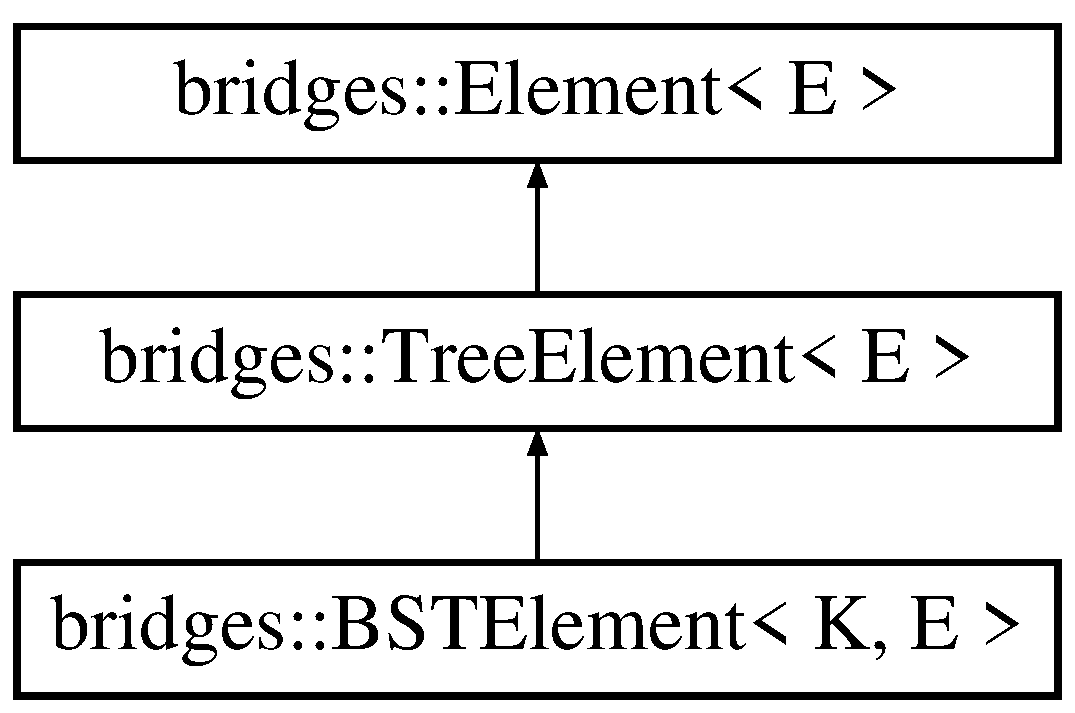
\includegraphics[height=3.000000cm]{classbridges_1_1_b_s_t_element}
\end{center}
\end{figure}
\subsection*{Public Member Functions}
\begin{DoxyCompactItemize}
\item 
\hyperlink{classbridges_1_1_b_s_t_element_a6bc4007042470785ca865c900bfbf20e}{B\+S\+T\+Element} ()
\item 
\hyperlink{classbridges_1_1_b_s_t_element_a0cb40809388f5191f3fc5f20c94e5cdd}{B\+S\+T\+Element} (const \hyperlink{classbridges_1_1_b_s_t_element}{B\+S\+T\+Element} \&bel)
\item 
\hyperlink{classbridges_1_1_b_s_t_element_ae9b41bdf1b056f450659735d51c3f459}{B\+S\+T\+Element} (E e, \hyperlink{classbridges_1_1_b_s_t_element}{B\+S\+T\+Element}$<$ K, E $>$ $\ast$left, \hyperlink{classbridges_1_1_b_s_t_element}{B\+S\+T\+Element}$<$ K, E $>$ $\ast$right)
\item 
\hyperlink{classbridges_1_1_b_s_t_element_ac491df9b8a9d2cf45a7a9f8f4f4e1857}{B\+S\+T\+Element} (K key, E e, \hyperlink{classbridges_1_1_b_s_t_element}{B\+S\+T\+Element}$<$ K, E $>$ $\ast$left, \hyperlink{classbridges_1_1_b_s_t_element}{B\+S\+T\+Element}$<$ K, E $>$ $\ast$right)
\item 
\hyperlink{classbridges_1_1_b_s_t_element_a19f2e875a88cf31fbbdfe37f316e5ee7}{B\+S\+T\+Element} (E e)
\item 
\hyperlink{classbridges_1_1_b_s_t_element_a7f839a433a77348edf2927a8ec86faf2}{B\+S\+T\+Element} (K key, E e)
\item 
\hyperlink{classbridges_1_1_b_s_t_element_abe6e9d2aa04a01cbcdd733067170b175}{B\+S\+T\+Element} (string label, K key, E e)
\item 
\hyperlink{classbridges_1_1_b_s_t_element_a43719ed15f0be72ef2977c829f7e770d}{B\+S\+T\+Element} (\hyperlink{classbridges_1_1_b_s_t_element}{B\+S\+T\+Element}$<$ K, E $>$ $\ast$left, \hyperlink{classbridges_1_1_b_s_t_element}{B\+S\+T\+Element}$<$ K, E $>$ $\ast$right)
\item 
K \hyperlink{classbridges_1_1_b_s_t_element_a89ce2cbf35d533d95ea89c14806f75f9}{get\+Key} ()
\item 
void \hyperlink{classbridges_1_1_b_s_t_element_a6d9008eaaf94d17b3376f419b964d6d0}{set\+Key} (K key)
\item 
\hyperlink{classbridges_1_1_b_s_t_element}{B\+S\+T\+Element}$<$ K, E $>$ $\ast$ \hyperlink{classbridges_1_1_b_s_t_element_aed62cfb1cc9c4954c19232193b8ec3bf}{get\+Left} ()
\item 
\hyperlink{classbridges_1_1_b_s_t_element}{B\+S\+T\+Element}$<$ K, E $>$ $\ast$ \hyperlink{classbridges_1_1_b_s_t_element_a6b1ef2135ded7cfdde9b4ac7c634a642}{get\+Right} ()
\item 
string \hyperlink{classbridges_1_1_b_s_t_element_a3c21670f445b662552bc3907a2ed51fd}{get\+Representation} ()
\end{DoxyCompactItemize}


\subsection{Constructor \& Destructor Documentation}
\hypertarget{classbridges_1_1_b_s_t_element_a6bc4007042470785ca865c900bfbf20e}{}\index{bridges\+::\+B\+S\+T\+Element@{bridges\+::\+B\+S\+T\+Element}!B\+S\+T\+Element@{B\+S\+T\+Element}}
\index{B\+S\+T\+Element@{B\+S\+T\+Element}!bridges\+::\+B\+S\+T\+Element@{bridges\+::\+B\+S\+T\+Element}}
\subsubsection[{B\+S\+T\+Element}]{\setlength{\rightskip}{0pt plus 5cm}template$<$typename K, typename E$>$ {\bf bridges\+::\+B\+S\+T\+Element}$<$ K, E $>$\+::{\bf B\+S\+T\+Element} (
\begin{DoxyParamCaption}
{}
\end{DoxyParamCaption}
)\hspace{0.3cm}{\ttfamily [inline]}}\label{classbridges_1_1_b_s_t_element_a6bc4007042470785ca865c900bfbf20e}
Construct an empty \hyperlink{classbridges_1_1_b_s_t_element}{B\+S\+T\+Element} with no key assigned and left and right pointers set to null. \hypertarget{classbridges_1_1_b_s_t_element_a0cb40809388f5191f3fc5f20c94e5cdd}{}\index{bridges\+::\+B\+S\+T\+Element@{bridges\+::\+B\+S\+T\+Element}!B\+S\+T\+Element@{B\+S\+T\+Element}}
\index{B\+S\+T\+Element@{B\+S\+T\+Element}!bridges\+::\+B\+S\+T\+Element@{bridges\+::\+B\+S\+T\+Element}}
\subsubsection[{B\+S\+T\+Element}]{\setlength{\rightskip}{0pt plus 5cm}template$<$typename K, typename E$>$ {\bf bridges\+::\+B\+S\+T\+Element}$<$ K, E $>$\+::{\bf B\+S\+T\+Element} (
\begin{DoxyParamCaption}
\item[{const {\bf B\+S\+T\+Element}$<$ K, E $>$ \&}]{bel}
\end{DoxyParamCaption}
)\hspace{0.3cm}{\ttfamily [inline]}}\label{classbridges_1_1_b_s_t_element_a0cb40809388f5191f3fc5f20c94e5cdd}
\hypertarget{classbridges_1_1_b_s_t_element_ae9b41bdf1b056f450659735d51c3f459}{}\index{bridges\+::\+B\+S\+T\+Element@{bridges\+::\+B\+S\+T\+Element}!B\+S\+T\+Element@{B\+S\+T\+Element}}
\index{B\+S\+T\+Element@{B\+S\+T\+Element}!bridges\+::\+B\+S\+T\+Element@{bridges\+::\+B\+S\+T\+Element}}
\subsubsection[{B\+S\+T\+Element}]{\setlength{\rightskip}{0pt plus 5cm}template$<$typename K, typename E$>$ {\bf bridges\+::\+B\+S\+T\+Element}$<$ K, E $>$\+::{\bf B\+S\+T\+Element} (
\begin{DoxyParamCaption}
\item[{E}]{e, }
\item[{{\bf B\+S\+T\+Element}$<$ K, E $>$ $\ast$}]{left, }
\item[{{\bf B\+S\+T\+Element}$<$ K, E $>$ $\ast$}]{right}
\end{DoxyParamCaption}
)\hspace{0.3cm}{\ttfamily [inline]}}\label{classbridges_1_1_b_s_t_element_ae9b41bdf1b056f450659735d51c3f459}
Construct a \hyperlink{classbridges_1_1_b_s_t_element}{B\+S\+T\+Element} holding an object \char`\"{}e\char`\"{} with a left pointer assigned to \char`\"{}left\char`\"{} and a right pointer assigned to \char`\"{}right\char`\"{}.


\begin{DoxyParams}{Parameters}
{\em e} & the object that \hyperlink{classbridges_1_1_b_s_t_element}{B\+S\+T\+Element} is holding \\
\hline
{\em left} & the \hyperlink{classbridges_1_1_b_s_t_element}{B\+S\+T\+Element} that should be assigned to the left pointer \\
\hline
{\em right} & the B\+S\+T\+Elemetn taht should be assigned to the right pointer \\
\hline
\end{DoxyParams}
\hypertarget{classbridges_1_1_b_s_t_element_ac491df9b8a9d2cf45a7a9f8f4f4e1857}{}\index{bridges\+::\+B\+S\+T\+Element@{bridges\+::\+B\+S\+T\+Element}!B\+S\+T\+Element@{B\+S\+T\+Element}}
\index{B\+S\+T\+Element@{B\+S\+T\+Element}!bridges\+::\+B\+S\+T\+Element@{bridges\+::\+B\+S\+T\+Element}}
\subsubsection[{B\+S\+T\+Element}]{\setlength{\rightskip}{0pt plus 5cm}template$<$typename K, typename E$>$ {\bf bridges\+::\+B\+S\+T\+Element}$<$ K, E $>$\+::{\bf B\+S\+T\+Element} (
\begin{DoxyParamCaption}
\item[{K}]{key, }
\item[{E}]{e, }
\item[{{\bf B\+S\+T\+Element}$<$ K, E $>$ $\ast$}]{left, }
\item[{{\bf B\+S\+T\+Element}$<$ K, E $>$ $\ast$}]{right}
\end{DoxyParamCaption}
)\hspace{0.3cm}{\ttfamily [inline]}}\label{classbridges_1_1_b_s_t_element_ac491df9b8a9d2cf45a7a9f8f4f4e1857}
Construct a \hyperlink{classbridges_1_1_b_s_t_element}{B\+S\+T\+Element} with a key \char`\"{}key\char`\"{}, holding an object \char`\"{}e\char`\"{} with a left pointer assigned to \char`\"{}left\char`\"{} and a right pointer assigned to \char`\"{}right\char`\"{}. 
\begin{DoxyParams}{Parameters}
{\em key} & the key to be used in a binary search tree implementation \\
\hline
{\em e} & the object this \hyperlink{classbridges_1_1_b_s_t_element}{B\+S\+T\+Element} is holding \\
\hline
{\em left} & the \hyperlink{classbridges_1_1_b_s_t_element}{B\+S\+T\+Element} that should be assigned to the left pointer \\
\hline
{\em right} & the \hyperlink{classbridges_1_1_b_s_t_element}{B\+S\+T\+Element} that should be assigned to the right pointer \\
\hline
\end{DoxyParams}
\hypertarget{classbridges_1_1_b_s_t_element_a19f2e875a88cf31fbbdfe37f316e5ee7}{}\index{bridges\+::\+B\+S\+T\+Element@{bridges\+::\+B\+S\+T\+Element}!B\+S\+T\+Element@{B\+S\+T\+Element}}
\index{B\+S\+T\+Element@{B\+S\+T\+Element}!bridges\+::\+B\+S\+T\+Element@{bridges\+::\+B\+S\+T\+Element}}
\subsubsection[{B\+S\+T\+Element}]{\setlength{\rightskip}{0pt plus 5cm}template$<$typename K, typename E$>$ {\bf bridges\+::\+B\+S\+T\+Element}$<$ K, E $>$\+::{\bf B\+S\+T\+Element} (
\begin{DoxyParamCaption}
\item[{E}]{e}
\end{DoxyParamCaption}
)\hspace{0.3cm}{\ttfamily [inline]}}\label{classbridges_1_1_b_s_t_element_a19f2e875a88cf31fbbdfe37f316e5ee7}
Construct a \hyperlink{classbridges_1_1_b_s_t_element}{B\+S\+T\+Element} holding the object \char`\"{}e\char`\"{}, with no key assigned and left and right pointers set to null. 
\begin{DoxyParams}{Parameters}
{\em e} & the object this \hyperlink{classbridges_1_1_b_s_t_element}{B\+S\+T\+Element} is holding \\
\hline
\end{DoxyParams}
\hypertarget{classbridges_1_1_b_s_t_element_a7f839a433a77348edf2927a8ec86faf2}{}\index{bridges\+::\+B\+S\+T\+Element@{bridges\+::\+B\+S\+T\+Element}!B\+S\+T\+Element@{B\+S\+T\+Element}}
\index{B\+S\+T\+Element@{B\+S\+T\+Element}!bridges\+::\+B\+S\+T\+Element@{bridges\+::\+B\+S\+T\+Element}}
\subsubsection[{B\+S\+T\+Element}]{\setlength{\rightskip}{0pt plus 5cm}template$<$typename K, typename E$>$ {\bf bridges\+::\+B\+S\+T\+Element}$<$ K, E $>$\+::{\bf B\+S\+T\+Element} (
\begin{DoxyParamCaption}
\item[{K}]{key, }
\item[{E}]{e}
\end{DoxyParamCaption}
)\hspace{0.3cm}{\ttfamily [inline]}}\label{classbridges_1_1_b_s_t_element_a7f839a433a77348edf2927a8ec86faf2}
Construct a \hyperlink{classbridges_1_1_b_s_t_element}{B\+S\+T\+Element} holding the object \char`\"{}e\char`\"{}, with key \char`\"{}key\char`\"{} assigned and left and right pointers set to null. 
\begin{DoxyParams}{Parameters}
{\em key} & the key to be used in a binary search tree implementation \\
\hline
{\em e} & the object this \hyperlink{classbridges_1_1_b_s_t_element}{B\+S\+T\+Element} is holding \\
\hline
\end{DoxyParams}
\hypertarget{classbridges_1_1_b_s_t_element_abe6e9d2aa04a01cbcdd733067170b175}{}\index{bridges\+::\+B\+S\+T\+Element@{bridges\+::\+B\+S\+T\+Element}!B\+S\+T\+Element@{B\+S\+T\+Element}}
\index{B\+S\+T\+Element@{B\+S\+T\+Element}!bridges\+::\+B\+S\+T\+Element@{bridges\+::\+B\+S\+T\+Element}}
\subsubsection[{B\+S\+T\+Element}]{\setlength{\rightskip}{0pt plus 5cm}template$<$typename K, typename E$>$ {\bf bridges\+::\+B\+S\+T\+Element}$<$ K, E $>$\+::{\bf B\+S\+T\+Element} (
\begin{DoxyParamCaption}
\item[{string}]{label, }
\item[{K}]{key, }
\item[{E}]{e}
\end{DoxyParamCaption}
)\hspace{0.3cm}{\ttfamily [inline]}}\label{classbridges_1_1_b_s_t_element_abe6e9d2aa04a01cbcdd733067170b175}
Construct a \hyperlink{classbridges_1_1_b_s_t_element}{B\+S\+T\+Element} holding the object \char`\"{}e\char`\"{}, with label set to \char`\"{}label\char`\"{}, with \char`\"{}key\char`\"{} assigned to key, and left and right pointers set to null. 
\begin{DoxyParams}{Parameters}
{\em label} & the label of \hyperlink{classbridges_1_1_b_s_t_element}{B\+S\+T\+Element} that shows up on the \hyperlink{classbridges_1_1_bridges}{Bridges} visualization \\
\hline
{\em key} & the key to be used in a binary search tree implementation \\
\hline
{\em e} & the object this \hyperlink{classbridges_1_1_b_s_t_element}{B\+S\+T\+Element} is holding \\
\hline
\end{DoxyParams}
\hypertarget{classbridges_1_1_b_s_t_element_a43719ed15f0be72ef2977c829f7e770d}{}\index{bridges\+::\+B\+S\+T\+Element@{bridges\+::\+B\+S\+T\+Element}!B\+S\+T\+Element@{B\+S\+T\+Element}}
\index{B\+S\+T\+Element@{B\+S\+T\+Element}!bridges\+::\+B\+S\+T\+Element@{bridges\+::\+B\+S\+T\+Element}}
\subsubsection[{B\+S\+T\+Element}]{\setlength{\rightskip}{0pt plus 5cm}template$<$typename K, typename E$>$ {\bf bridges\+::\+B\+S\+T\+Element}$<$ K, E $>$\+::{\bf B\+S\+T\+Element} (
\begin{DoxyParamCaption}
\item[{{\bf B\+S\+T\+Element}$<$ K, E $>$ $\ast$}]{left, }
\item[{{\bf B\+S\+T\+Element}$<$ K, E $>$ $\ast$}]{right}
\end{DoxyParamCaption}
)\hspace{0.3cm}{\ttfamily [inline]}}\label{classbridges_1_1_b_s_t_element_a43719ed15f0be72ef2977c829f7e770d}
Construct an empty \hyperlink{classbridges_1_1_b_s_t_element}{B\+S\+T\+Element}, with no key assigned, and left and right pointers set to null. 
\begin{DoxyParams}{Parameters}
{\em left} & the \hyperlink{classbridges_1_1_b_s_t_element}{B\+S\+T\+Element} that should be assigned to the left pointer \\
\hline
{\em right} & the \hyperlink{classbridges_1_1_b_s_t_element}{B\+S\+T\+Element} that should be assigned to the right pointer \\
\hline
\end{DoxyParams}


\subsection{Member Function Documentation}
\hypertarget{classbridges_1_1_b_s_t_element_a89ce2cbf35d533d95ea89c14806f75f9}{}\index{bridges\+::\+B\+S\+T\+Element@{bridges\+::\+B\+S\+T\+Element}!get\+Key@{get\+Key}}
\index{get\+Key@{get\+Key}!bridges\+::\+B\+S\+T\+Element@{bridges\+::\+B\+S\+T\+Element}}
\subsubsection[{get\+Key}]{\setlength{\rightskip}{0pt plus 5cm}template$<$typename K, typename E$>$ K {\bf bridges\+::\+B\+S\+T\+Element}$<$ K, E $>$\+::get\+Key (
\begin{DoxyParamCaption}
{}
\end{DoxyParamCaption}
)\hspace{0.3cm}{\ttfamily [inline]}}\label{classbridges_1_1_b_s_t_element_a89ce2cbf35d533d95ea89c14806f75f9}
Return the key of the \hyperlink{classbridges_1_1_b_s_t_element}{B\+S\+T\+Element} \begin{DoxyReturn}{Returns}
the key of this \hyperlink{classbridges_1_1_b_s_t_element}{B\+S\+T\+Element} 
\end{DoxyReturn}
\hypertarget{classbridges_1_1_b_s_t_element_aed62cfb1cc9c4954c19232193b8ec3bf}{}\index{bridges\+::\+B\+S\+T\+Element@{bridges\+::\+B\+S\+T\+Element}!get\+Left@{get\+Left}}
\index{get\+Left@{get\+Left}!bridges\+::\+B\+S\+T\+Element@{bridges\+::\+B\+S\+T\+Element}}
\subsubsection[{get\+Left}]{\setlength{\rightskip}{0pt plus 5cm}template$<$typename K, typename E$>$ {\bf B\+S\+T\+Element}$<$K,E$>$$\ast$ {\bf bridges\+::\+B\+S\+T\+Element}$<$ K, E $>$\+::get\+Left (
\begin{DoxyParamCaption}
{}
\end{DoxyParamCaption}
)\hspace{0.3cm}{\ttfamily [inline]}}\label{classbridges_1_1_b_s_t_element_aed62cfb1cc9c4954c19232193b8ec3bf}
get Left child

\begin{DoxyReturn}{Returns}
left child pointer (from parent) 
\end{DoxyReturn}
\hypertarget{classbridges_1_1_b_s_t_element_a3c21670f445b662552bc3907a2ed51fd}{}\index{bridges\+::\+B\+S\+T\+Element@{bridges\+::\+B\+S\+T\+Element}!get\+Representation@{get\+Representation}}
\index{get\+Representation@{get\+Representation}!bridges\+::\+B\+S\+T\+Element@{bridges\+::\+B\+S\+T\+Element}}
\subsubsection[{get\+Representation}]{\setlength{\rightskip}{0pt plus 5cm}template$<$typename K, typename E$>$ string {\bf bridges\+::\+B\+S\+T\+Element}$<$ K, E $>$\+::get\+Representation (
\begin{DoxyParamCaption}
{}
\end{DoxyParamCaption}
)\hspace{0.3cm}{\ttfamily [inline]}}\label{classbridges_1_1_b_s_t_element_a3c21670f445b662552bc3907a2ed51fd}
, must include key get J\+S\+O\+N of node representation

\begin{DoxyReturn}{Returns}
J\+S\+O\+N of the node representation 
\end{DoxyReturn}
\hypertarget{classbridges_1_1_b_s_t_element_a6b1ef2135ded7cfdde9b4ac7c634a642}{}\index{bridges\+::\+B\+S\+T\+Element@{bridges\+::\+B\+S\+T\+Element}!get\+Right@{get\+Right}}
\index{get\+Right@{get\+Right}!bridges\+::\+B\+S\+T\+Element@{bridges\+::\+B\+S\+T\+Element}}
\subsubsection[{get\+Right}]{\setlength{\rightskip}{0pt plus 5cm}template$<$typename K, typename E$>$ {\bf B\+S\+T\+Element}$<$K,E$>$$\ast$ {\bf bridges\+::\+B\+S\+T\+Element}$<$ K, E $>$\+::get\+Right (
\begin{DoxyParamCaption}
{}
\end{DoxyParamCaption}
)\hspace{0.3cm}{\ttfamily [inline]}}\label{classbridges_1_1_b_s_t_element_a6b1ef2135ded7cfdde9b4ac7c634a642}
\hypertarget{classbridges_1_1_b_s_t_element_a6d9008eaaf94d17b3376f419b964d6d0}{}\index{bridges\+::\+B\+S\+T\+Element@{bridges\+::\+B\+S\+T\+Element}!set\+Key@{set\+Key}}
\index{set\+Key@{set\+Key}!bridges\+::\+B\+S\+T\+Element@{bridges\+::\+B\+S\+T\+Element}}
\subsubsection[{set\+Key}]{\setlength{\rightskip}{0pt plus 5cm}template$<$typename K, typename E$>$ void {\bf bridges\+::\+B\+S\+T\+Element}$<$ K, E $>$\+::set\+Key (
\begin{DoxyParamCaption}
\item[{K}]{key}
\end{DoxyParamCaption}
)\hspace{0.3cm}{\ttfamily [inline]}}\label{classbridges_1_1_b_s_t_element_a6d9008eaaf94d17b3376f419b964d6d0}
Set the key of the \hyperlink{classbridges_1_1_b_s_t_element}{B\+S\+T\+Element} to key 
\begin{DoxyParams}{Parameters}
{\em key} & the key to set \\
\hline
\end{DoxyParams}


The documentation for this class was generated from the following file\+:\begin{DoxyCompactItemize}
\item 
src/\hyperlink{_b_s_t_element_8h}{B\+S\+T\+Element.\+h}\end{DoxyCompactItemize}

\hypertarget{classbridges_1_1_connector}{}\section{bridges\+:\+:Connector Class Reference}
\label{classbridges_1_1_connector}\index{bridges\+::\+Connector@{bridges\+::\+Connector}}


{\ttfamily \#include $<$Connector.\+h$>$}

\subsection*{Public Member Functions}
\begin{DoxyCompactItemize}
\item 
\hyperlink{classbridges_1_1_connector_ac623bc6df7c8bf2d0170ebb5bbbc13bf}{Connector} ()
\item 
string \hyperlink{classbridges_1_1_connector_a509ca5ef39f5d8ee5a4f6c0dd9228f8f}{get\+Server\+U\+R\+L} ()
\item 
void \hyperlink{classbridges_1_1_connector_a92ae43e609323c039ca8ca0800f88288}{set\+Server\+U\+R\+L} (string url)
\item 
void \hyperlink{classbridges_1_1_connector_a6ea360ff4c37ae03a81ec0ac44ec8740}{post} (string url, string json\+\_\+of\+\_\+ds)
\end{DoxyCompactItemize}


\subsection{Constructor \& Destructor Documentation}
\hypertarget{classbridges_1_1_connector_ac623bc6df7c8bf2d0170ebb5bbbc13bf}{}\index{bridges\+::\+Connector@{bridges\+::\+Connector}!Connector@{Connector}}
\index{Connector@{Connector}!bridges\+::\+Connector@{bridges\+::\+Connector}}
\subsubsection[{Connector}]{\setlength{\rightskip}{0pt plus 5cm}bridges\+::\+Connector\+::\+Connector (
\begin{DoxyParamCaption}
{}
\end{DoxyParamCaption}
)\hspace{0.3cm}{\ttfamily [inline]}}\label{classbridges_1_1_connector_ac623bc6df7c8bf2d0170ebb5bbbc13bf}


\subsection{Member Function Documentation}
\hypertarget{classbridges_1_1_connector_a509ca5ef39f5d8ee5a4f6c0dd9228f8f}{}\index{bridges\+::\+Connector@{bridges\+::\+Connector}!get\+Server\+U\+R\+L@{get\+Server\+U\+R\+L}}
\index{get\+Server\+U\+R\+L@{get\+Server\+U\+R\+L}!bridges\+::\+Connector@{bridges\+::\+Connector}}
\subsubsection[{get\+Server\+U\+R\+L}]{\setlength{\rightskip}{0pt plus 5cm}string bridges\+::\+Connector\+::get\+Server\+U\+R\+L (
\begin{DoxyParamCaption}
{}
\end{DoxyParamCaption}
)\hspace{0.3cm}{\ttfamily [inline]}}\label{classbridges_1_1_connector_a509ca5ef39f5d8ee5a4f6c0dd9228f8f}
Get the current base U\+R\+L for the Data\+Formatters server (with no ending /) \begin{DoxyReturn}{Returns}

\end{DoxyReturn}
\hypertarget{classbridges_1_1_connector_a6ea360ff4c37ae03a81ec0ac44ec8740}{}\index{bridges\+::\+Connector@{bridges\+::\+Connector}!post@{post}}
\index{post@{post}!bridges\+::\+Connector@{bridges\+::\+Connector}}
\subsubsection[{post}]{\setlength{\rightskip}{0pt plus 5cm}void bridges\+::\+Connector\+::post (
\begin{DoxyParamCaption}
\item[{string}]{url, }
\item[{string}]{json\+\_\+of\+\_\+ds}
\end{DoxyParamCaption}
)\hspace{0.3cm}{\ttfamily [inline]}}\label{classbridges_1_1_connector_a6ea360ff4c37ae03a81ec0ac44ec8740}
Execute a simple P\+O\+S\+T request with relative paths, of request parameters.

Uses the Curl library \hypertarget{classbridges_1_1_connector_a92ae43e609323c039ca8ca0800f88288}{}\index{bridges\+::\+Connector@{bridges\+::\+Connector}!set\+Server\+U\+R\+L@{set\+Server\+U\+R\+L}}
\index{set\+Server\+U\+R\+L@{set\+Server\+U\+R\+L}!bridges\+::\+Connector@{bridges\+::\+Connector}}
\subsubsection[{set\+Server\+U\+R\+L}]{\setlength{\rightskip}{0pt plus 5cm}void bridges\+::\+Connector\+::set\+Server\+U\+R\+L (
\begin{DoxyParamCaption}
\item[{string}]{url}
\end{DoxyParamCaption}
)\hspace{0.3cm}{\ttfamily [inline]}}\label{classbridges_1_1_connector_a92ae43e609323c039ca8ca0800f88288}
Set the current base U\+R\+L for the Data\+Formatters server (with no ending /) 
\begin{DoxyParams}{Parameters}
{\em server\+\_\+url} & \\
\hline
\end{DoxyParams}


The documentation for this class was generated from the following file\+:\begin{DoxyCompactItemize}
\item 
src/\hyperlink{_connector_8h}{Connector.\+h}\end{DoxyCompactItemize}

\hypertarget{classbridges_1_1_d_lelement}{}\section{bridges\+:\+:D\+Lelement$<$ E $>$ Class Template Reference}
\label{classbridges_1_1_d_lelement}\index{bridges\+::\+D\+Lelement$<$ E $>$@{bridges\+::\+D\+Lelement$<$ E $>$}}


{\ttfamily \#include $<$D\+Lelement.\+h$>$}

Inheritance diagram for bridges\+:\+:D\+Lelement$<$ E $>$\+:\begin{figure}[H]
\begin{center}
\leavevmode
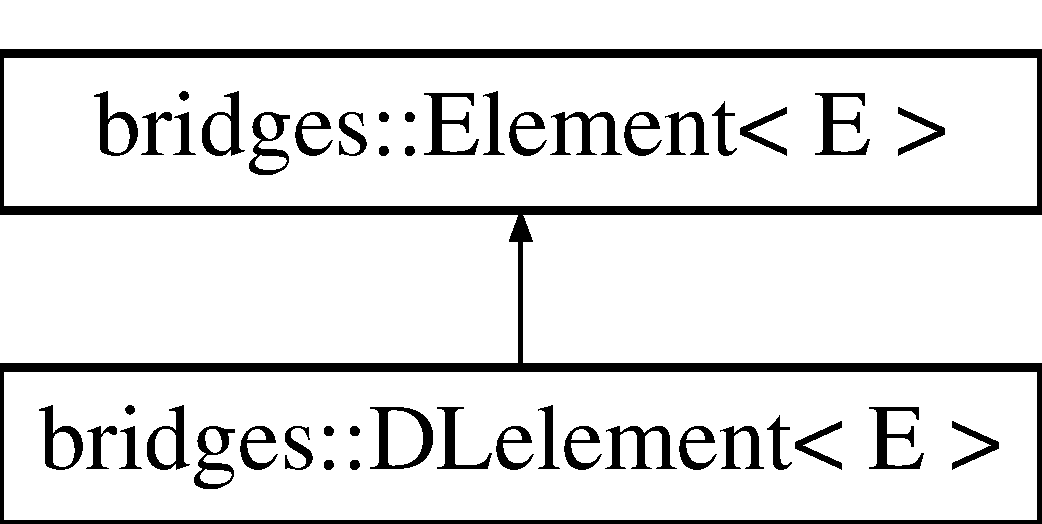
\includegraphics[height=2.000000cm]{classbridges_1_1_d_lelement}
\end{center}
\end{figure}
\subsection*{Public Member Functions}
\begin{DoxyCompactItemize}
\item 
\hyperlink{classbridges_1_1_d_lelement_a79e05d2d74eab75a987531250037b40b}{D\+Lelement} ()
\item 
\hyperlink{classbridges_1_1_d_lelement_af2e5ada14a837f8e01001531ec1c76a7}{D\+Lelement} (const \hyperlink{classbridges_1_1_d_lelement}{D\+Lelement}$<$ E $>$ \&dle)
\item 
\hyperlink{classbridges_1_1_d_lelement_a1897fad94722f833241e7a665fe57124}{D\+Lelement} (string label, E e)
\item 
\hyperlink{classbridges_1_1_d_lelement_a07dabe0accc1bbdd4063a566b1f02f94}{D\+Lelement} (\hyperlink{classbridges_1_1_d_lelement}{D\+Lelement}$<$ E $>$ $\ast$next, \hyperlink{classbridges_1_1_d_lelement}{D\+Lelement}$<$ E $>$ $\ast$prev)
\item 
\hyperlink{classbridges_1_1_d_lelement_a5fd70407e3539971d76d8b204e775f9f}{D\+Lelement} (E e, \hyperlink{classbridges_1_1_d_lelement}{D\+Lelement}$<$ E $>$ $\ast$next, \hyperlink{classbridges_1_1_d_lelement}{D\+Lelement}$<$ E $>$ $\ast$prev)
\item 
\hyperlink{classbridges_1_1_d_lelement}{D\+Lelement}$<$ E $>$ $\ast$ \hyperlink{classbridges_1_1_d_lelement_a0f638cca77375d6bdc2ff8a23700568c}{get\+Next} ()
\item 
void \hyperlink{classbridges_1_1_d_lelement_a12db627afdb6e0c56ead5f46a3d41036}{set\+Next} (\hyperlink{classbridges_1_1_d_lelement}{D\+Lelement}$<$ E $>$ $\ast$next)
\item 
\hyperlink{classbridges_1_1_d_lelement}{D\+Lelement}$<$ E $>$ $\ast$ \hyperlink{classbridges_1_1_d_lelement_aa3093474809715575f4c5145d71e6db9}{get\+Prev} ()
\item 
void \hyperlink{classbridges_1_1_d_lelement_adcf1c913e922a15724e8cd86c21c5730}{set\+Prev} (\hyperlink{classbridges_1_1_d_lelement}{D\+Lelement}$<$ E $>$ $\ast$prev)
\end{DoxyCompactItemize}


\subsection{Constructor \& Destructor Documentation}
\hypertarget{classbridges_1_1_d_lelement_a79e05d2d74eab75a987531250037b40b}{}\index{bridges\+::\+D\+Lelement@{bridges\+::\+D\+Lelement}!D\+Lelement@{D\+Lelement}}
\index{D\+Lelement@{D\+Lelement}!bridges\+::\+D\+Lelement@{bridges\+::\+D\+Lelement}}
\subsubsection[{D\+Lelement}]{\setlength{\rightskip}{0pt plus 5cm}template$<$typename E$>$ {\bf bridges\+::\+D\+Lelement}$<$ E $>$\+::{\bf D\+Lelement} (
\begin{DoxyParamCaption}
{}
\end{DoxyParamCaption}
)\hspace{0.3cm}{\ttfamily [inline]}}\label{classbridges_1_1_d_lelement_a79e05d2d74eab75a987531250037b40b}
Constructs an empty \hyperlink{classbridges_1_1_d_lelement}{D\+Lelement} with next and prev pointers set to N\+U\+L\+L. \hypertarget{classbridges_1_1_d_lelement_af2e5ada14a837f8e01001531ec1c76a7}{}\index{bridges\+::\+D\+Lelement@{bridges\+::\+D\+Lelement}!D\+Lelement@{D\+Lelement}}
\index{D\+Lelement@{D\+Lelement}!bridges\+::\+D\+Lelement@{bridges\+::\+D\+Lelement}}
\subsubsection[{D\+Lelement}]{\setlength{\rightskip}{0pt plus 5cm}template$<$typename E$>$ {\bf bridges\+::\+D\+Lelement}$<$ E $>$\+::{\bf D\+Lelement} (
\begin{DoxyParamCaption}
\item[{const {\bf D\+Lelement}$<$ E $>$ \&}]{dle}
\end{DoxyParamCaption}
)\hspace{0.3cm}{\ttfamily [inline]}}\label{classbridges_1_1_d_lelement_af2e5ada14a837f8e01001531ec1c76a7}
\hypertarget{classbridges_1_1_d_lelement_a1897fad94722f833241e7a665fe57124}{}\index{bridges\+::\+D\+Lelement@{bridges\+::\+D\+Lelement}!D\+Lelement@{D\+Lelement}}
\index{D\+Lelement@{D\+Lelement}!bridges\+::\+D\+Lelement@{bridges\+::\+D\+Lelement}}
\subsubsection[{D\+Lelement}]{\setlength{\rightskip}{0pt plus 5cm}template$<$typename E$>$ {\bf bridges\+::\+D\+Lelement}$<$ E $>$\+::{\bf D\+Lelement} (
\begin{DoxyParamCaption}
\item[{string}]{label, }
\item[{E}]{e}
\end{DoxyParamCaption}
)\hspace{0.3cm}{\ttfamily [inline]}}\label{classbridges_1_1_d_lelement_a1897fad94722f833241e7a665fe57124}
Constructs a \hyperlink{classbridges_1_1_d_lelement}{D\+Lelement} labeled \char`\"{}label\char`\"{}, holding an object \char`\"{}e\char`\"{}, with next and prev pointers set to null. 
\begin{DoxyParams}{Parameters}
{\em label} & the label for this \hyperlink{classbridges_1_1_d_lelement}{D\+Lelement} that shows up on the \hyperlink{classbridges_1_1_bridges}{Bridges} visualization \\
\hline
{\em e} & the genereic object that this \hyperlink{classbridges_1_1_d_lelement}{D\+Lelement} is holding \\
\hline
\end{DoxyParams}
\hypertarget{classbridges_1_1_d_lelement_a07dabe0accc1bbdd4063a566b1f02f94}{}\index{bridges\+::\+D\+Lelement@{bridges\+::\+D\+Lelement}!D\+Lelement@{D\+Lelement}}
\index{D\+Lelement@{D\+Lelement}!bridges\+::\+D\+Lelement@{bridges\+::\+D\+Lelement}}
\subsubsection[{D\+Lelement}]{\setlength{\rightskip}{0pt plus 5cm}template$<$typename E$>$ {\bf bridges\+::\+D\+Lelement}$<$ E $>$\+::{\bf D\+Lelement} (
\begin{DoxyParamCaption}
\item[{{\bf D\+Lelement}$<$ E $>$ $\ast$}]{next, }
\item[{{\bf D\+Lelement}$<$ E $>$ $\ast$}]{prev}
\end{DoxyParamCaption}
)\hspace{0.3cm}{\ttfamily [inline]}}\label{classbridges_1_1_d_lelement_a07dabe0accc1bbdd4063a566b1f02f94}
Constructs an empty \hyperlink{classbridges_1_1_d_lelement}{D\+Lelement} with the next pointer set to the \hyperlink{classbridges_1_1_d_lelement}{D\+Lelement} \char`\"{}next\char`\"{} and the prev pointer set to \hyperlink{classbridges_1_1_d_lelement}{D\+Lelement} \char`\"{}prev\char`\"{}. 
\begin{DoxyParams}{Parameters}
{\em next} & the \hyperlink{classbridges_1_1_d_lelement}{D\+Lelement} that should be assigned to the next pointer \\
\hline
{\em prev} & the \hyperlink{classbridges_1_1_d_lelement}{D\+Lelement} that should be assigned to the prev pointer \\
\hline
\end{DoxyParams}
\hypertarget{classbridges_1_1_d_lelement_a5fd70407e3539971d76d8b204e775f9f}{}\index{bridges\+::\+D\+Lelement@{bridges\+::\+D\+Lelement}!D\+Lelement@{D\+Lelement}}
\index{D\+Lelement@{D\+Lelement}!bridges\+::\+D\+Lelement@{bridges\+::\+D\+Lelement}}
\subsubsection[{D\+Lelement}]{\setlength{\rightskip}{0pt plus 5cm}template$<$typename E$>$ {\bf bridges\+::\+D\+Lelement}$<$ E $>$\+::{\bf D\+Lelement} (
\begin{DoxyParamCaption}
\item[{E}]{e, }
\item[{{\bf D\+Lelement}$<$ E $>$ $\ast$}]{next, }
\item[{{\bf D\+Lelement}$<$ E $>$ $\ast$}]{prev}
\end{DoxyParamCaption}
)\hspace{0.3cm}{\ttfamily [inline]}}\label{classbridges_1_1_d_lelement_a5fd70407e3539971d76d8b204e775f9f}
Constructs a \hyperlink{classbridges_1_1_d_lelement}{D\+Lelement} holding an object \char`\"{}e\char`\"{}, with the next pointer set to the \hyperlink{classbridges_1_1_d_lelement}{D\+Lelement} \char`\"{}next\char`\"{} and the prev pointer set to \hyperlink{classbridges_1_1_d_lelement}{D\+Lelement} \char`\"{}prev\char`\"{}. 
\begin{DoxyParams}{Parameters}
{\em e} & the genereic object that this \hyperlink{classbridges_1_1_d_lelement}{D\+Lelement} is holding \\
\hline
{\em next} & the \hyperlink{classbridges_1_1_d_lelement}{D\+Lelement} that should be assigned to the next pointer \\
\hline
{\em prev} & the \hyperlink{classbridges_1_1_d_lelement}{D\+Lelement} that should be assigned to the prev pointer \\
\hline
\end{DoxyParams}


\subsection{Member Function Documentation}
\hypertarget{classbridges_1_1_d_lelement_a0f638cca77375d6bdc2ff8a23700568c}{}\index{bridges\+::\+D\+Lelement@{bridges\+::\+D\+Lelement}!get\+Next@{get\+Next}}
\index{get\+Next@{get\+Next}!bridges\+::\+D\+Lelement@{bridges\+::\+D\+Lelement}}
\subsubsection[{get\+Next}]{\setlength{\rightskip}{0pt plus 5cm}template$<$typename E$>$ {\bf D\+Lelement}$<$E$>$$\ast$ {\bf bridges\+::\+D\+Lelement}$<$ E $>$\+::get\+Next (
\begin{DoxyParamCaption}
{}
\end{DoxyParamCaption}
)\hspace{0.3cm}{\ttfamily [inline]}}\label{classbridges_1_1_d_lelement_a0f638cca77375d6bdc2ff8a23700568c}
This method returns the pointer to the next \hyperlink{classbridges_1_1_d_lelement}{D\+Lelement} \begin{DoxyReturn}{Returns}
the \hyperlink{classbridges_1_1_d_lelement}{D\+Lelement} assigned to the next pointer 
\end{DoxyReturn}
\hypertarget{classbridges_1_1_d_lelement_aa3093474809715575f4c5145d71e6db9}{}\index{bridges\+::\+D\+Lelement@{bridges\+::\+D\+Lelement}!get\+Prev@{get\+Prev}}
\index{get\+Prev@{get\+Prev}!bridges\+::\+D\+Lelement@{bridges\+::\+D\+Lelement}}
\subsubsection[{get\+Prev}]{\setlength{\rightskip}{0pt plus 5cm}template$<$typename E$>$ {\bf D\+Lelement}$<$E$>$$\ast$ {\bf bridges\+::\+D\+Lelement}$<$ E $>$\+::get\+Prev (
\begin{DoxyParamCaption}
{}
\end{DoxyParamCaption}
)\hspace{0.3cm}{\ttfamily [inline]}}\label{classbridges_1_1_d_lelement_aa3093474809715575f4c5145d71e6db9}
This method returns the pointer to the previous \hyperlink{classbridges_1_1_d_lelement}{D\+Lelement} \begin{DoxyReturn}{Returns}
the \hyperlink{classbridges_1_1_d_lelement}{D\+Lelement} assigned to the prev pointer 
\end{DoxyReturn}
\hypertarget{classbridges_1_1_d_lelement_a12db627afdb6e0c56ead5f46a3d41036}{}\index{bridges\+::\+D\+Lelement@{bridges\+::\+D\+Lelement}!set\+Next@{set\+Next}}
\index{set\+Next@{set\+Next}!bridges\+::\+D\+Lelement@{bridges\+::\+D\+Lelement}}
\subsubsection[{set\+Next}]{\setlength{\rightskip}{0pt plus 5cm}template$<$typename E$>$ void {\bf bridges\+::\+D\+Lelement}$<$ E $>$\+::set\+Next (
\begin{DoxyParamCaption}
\item[{{\bf D\+Lelement}$<$ E $>$ $\ast$}]{next}
\end{DoxyParamCaption}
)\hspace{0.3cm}{\ttfamily [inline]}}\label{classbridges_1_1_d_lelement_a12db627afdb6e0c56ead5f46a3d41036}
This method sets the pointer to the next \hyperlink{classbridges_1_1_d_lelement}{D\+Lelement} 
\begin{DoxyParams}{Parameters}
{\em next} & the \hyperlink{classbridges_1_1_d_lelement}{D\+Lelement} that should be assigned to the next pointer \\
\hline
\end{DoxyParams}
\hypertarget{classbridges_1_1_d_lelement_adcf1c913e922a15724e8cd86c21c5730}{}\index{bridges\+::\+D\+Lelement@{bridges\+::\+D\+Lelement}!set\+Prev@{set\+Prev}}
\index{set\+Prev@{set\+Prev}!bridges\+::\+D\+Lelement@{bridges\+::\+D\+Lelement}}
\subsubsection[{set\+Prev}]{\setlength{\rightskip}{0pt plus 5cm}template$<$typename E$>$ void {\bf bridges\+::\+D\+Lelement}$<$ E $>$\+::set\+Prev (
\begin{DoxyParamCaption}
\item[{{\bf D\+Lelement}$<$ E $>$ $\ast$}]{prev}
\end{DoxyParamCaption}
)\hspace{0.3cm}{\ttfamily [inline]}}\label{classbridges_1_1_d_lelement_adcf1c913e922a15724e8cd86c21c5730}
This method sets the pointer to the previous \hyperlink{classbridges_1_1_d_lelement}{D\+Lelement} 
\begin{DoxyParams}{Parameters}
{\em prev} & the \hyperlink{classbridges_1_1_d_lelement}{D\+Lelement} that should be assigned to the prev pointer \\
\hline
\end{DoxyParams}


The documentation for this class was generated from the following file\+:\begin{DoxyCompactItemize}
\item 
src/\hyperlink{_d_lelement_8h}{D\+Lelement.\+h}\end{DoxyCompactItemize}

\hypertarget{classbridges_1_1_edge}{}\section{bridges\+:\+:Edge$<$ Key $>$ Class Template Reference}
\label{classbridges_1_1_edge}\index{bridges\+::\+Edge$<$ Key $>$@{bridges\+::\+Edge$<$ Key $>$}}


{\ttfamily \#include $<$Edge.\+h$>$}

\subsection*{Public Member Functions}
\begin{DoxyCompactItemize}
\item 
\hyperlink{classbridges_1_1_edge_aa829f4c7a2c7674dcbbb649dc3dc7996}{Edge} ()
\item 
\hyperlink{classbridges_1_1_edge_aae34da5b01b0663b5ca1cb724872fd7d}{Edge} (int wt)
\item 
\hyperlink{classbridges_1_1_edge_a63e84d686135b5a9158b36819d422ea2}{Edge} (int wt, Key v)
\item 
void \hyperlink{classbridges_1_1_edge_a404b1be315c3ba5a7da48d22750fd90f}{set\+Weight} (int wt)
\item 
int \hyperlink{classbridges_1_1_edge_abb0a90b93b1ee135dd19464780d25620}{get\+Weight} ()
\item 
void \hyperlink{classbridges_1_1_edge_a5b6df66e9af59226d2692b7057eeea37}{set\+Vertex} (Key v)
\item 
Key \hyperlink{classbridges_1_1_edge_aa604e71bc9068ca68d95e49adcf63920}{get\+Vertex} ()
\item 
void \hyperlink{classbridges_1_1_edge_ab21c0f917e8a3a40e871fb49957103ba}{set\+Edge\+Data} (string data)
\item 
string \hyperlink{classbridges_1_1_edge_a3bc88f8f713f29a207ff572d9f8fead6}{get\+Edge\+Data} ()
\item 
void \hyperlink{classbridges_1_1_edge_af9aff4af3f19becfaf4b05369c25c0ce}{set\+Edge} (int wt, Key v)
\item 
\hyperlink{classbridges_1_1_edge}{Edge} $\ast$ \hyperlink{classbridges_1_1_edge_acc1b8dd71672737ede797a5b24b64c4a}{get\+Edge} ()
\end{DoxyCompactItemize}


\subsection{Constructor \& Destructor Documentation}
\hypertarget{classbridges_1_1_edge_aa829f4c7a2c7674dcbbb649dc3dc7996}{}\index{bridges\+::\+Edge@{bridges\+::\+Edge}!Edge@{Edge}}
\index{Edge@{Edge}!bridges\+::\+Edge@{bridges\+::\+Edge}}
\subsubsection[{Edge}]{\setlength{\rightskip}{0pt plus 5cm}template$<$typename Key$>$ {\bf bridges\+::\+Edge}$<$ Key $>$\+::{\bf Edge} (
\begin{DoxyParamCaption}
{}
\end{DoxyParamCaption}
)\hspace{0.3cm}{\ttfamily [inline]}}\label{classbridges_1_1_edge_aa829f4c7a2c7674dcbbb649dc3dc7996}
Construct an edge with no terminating \hyperlink{classbridges_1_1_element}{Element} -\/ used only for graphs \hypertarget{classbridges_1_1_edge_aae34da5b01b0663b5ca1cb724872fd7d}{}\index{bridges\+::\+Edge@{bridges\+::\+Edge}!Edge@{Edge}}
\index{Edge@{Edge}!bridges\+::\+Edge@{bridges\+::\+Edge}}
\subsubsection[{Edge}]{\setlength{\rightskip}{0pt plus 5cm}template$<$typename Key$>$ {\bf bridges\+::\+Edge}$<$ Key $>$\+::{\bf Edge} (
\begin{DoxyParamCaption}
\item[{int}]{wt}
\end{DoxyParamCaption}
)\hspace{0.3cm}{\ttfamily [inline]}}\label{classbridges_1_1_edge_aae34da5b01b0663b5ca1cb724872fd7d}
Construct an edge with thickness equal to \char`\"{}wt\char`\"{} and no terminating \hyperlink{classbridges_1_1_element}{Element}, used only for graphs. 
\begin{DoxyParams}{Parameters}
{\em wt} & integer representing edge weight, \\
\hline
\end{DoxyParams}
\hypertarget{classbridges_1_1_edge_a63e84d686135b5a9158b36819d422ea2}{}\index{bridges\+::\+Edge@{bridges\+::\+Edge}!Edge@{Edge}}
\index{Edge@{Edge}!bridges\+::\+Edge@{bridges\+::\+Edge}}
\subsubsection[{Edge}]{\setlength{\rightskip}{0pt plus 5cm}template$<$typename Key$>$ {\bf bridges\+::\+Edge}$<$ Key $>$\+::{\bf Edge} (
\begin{DoxyParamCaption}
\item[{int}]{wt, }
\item[{Key}]{v}
\end{DoxyParamCaption}
)\hspace{0.3cm}{\ttfamily [inline]}}\label{classbridges_1_1_edge_a63e84d686135b5a9158b36819d422ea2}
Construct an edge, given edge weight and terminating vertex 
\begin{DoxyParams}{Parameters}
{\em wt} & integer representing the edge weight(application dependent) \\
\hline
{\em v} & terminating vertex id \\
\hline
\end{DoxyParams}


\subsection{Member Function Documentation}
\hypertarget{classbridges_1_1_edge_acc1b8dd71672737ede797a5b24b64c4a}{}\index{bridges\+::\+Edge@{bridges\+::\+Edge}!get\+Edge@{get\+Edge}}
\index{get\+Edge@{get\+Edge}!bridges\+::\+Edge@{bridges\+::\+Edge}}
\subsubsection[{get\+Edge}]{\setlength{\rightskip}{0pt plus 5cm}template$<$typename Key$>$ {\bf Edge}$\ast$ {\bf bridges\+::\+Edge}$<$ Key $>$\+::get\+Edge (
\begin{DoxyParamCaption}
{}
\end{DoxyParamCaption}
)\hspace{0.3cm}{\ttfamily [inline]}}\label{classbridges_1_1_edge_acc1b8dd71672737ede797a5b24b64c4a}
Returns this edge \hypertarget{classbridges_1_1_edge_a3bc88f8f713f29a207ff572d9f8fead6}{}\index{bridges\+::\+Edge@{bridges\+::\+Edge}!get\+Edge\+Data@{get\+Edge\+Data}}
\index{get\+Edge\+Data@{get\+Edge\+Data}!bridges\+::\+Edge@{bridges\+::\+Edge}}
\subsubsection[{get\+Edge\+Data}]{\setlength{\rightskip}{0pt plus 5cm}template$<$typename Key$>$ string {\bf bridges\+::\+Edge}$<$ Key $>$\+::get\+Edge\+Data (
\begin{DoxyParamCaption}
{}
\end{DoxyParamCaption}
)\hspace{0.3cm}{\ttfamily [inline]}}\label{classbridges_1_1_edge_a3bc88f8f713f29a207ff572d9f8fead6}
Get edge data

\begin{DoxyReturn}{Returns}
the edge data 
\end{DoxyReturn}
\hypertarget{classbridges_1_1_edge_aa604e71bc9068ca68d95e49adcf63920}{}\index{bridges\+::\+Edge@{bridges\+::\+Edge}!get\+Vertex@{get\+Vertex}}
\index{get\+Vertex@{get\+Vertex}!bridges\+::\+Edge@{bridges\+::\+Edge}}
\subsubsection[{get\+Vertex}]{\setlength{\rightskip}{0pt plus 5cm}template$<$typename Key$>$ Key {\bf bridges\+::\+Edge}$<$ Key $>$\+::get\+Vertex (
\begin{DoxyParamCaption}
{}
\end{DoxyParamCaption}
)\hspace{0.3cm}{\ttfamily [inline]}}\label{classbridges_1_1_edge_aa604e71bc9068ca68d95e49adcf63920}
Get identifer of the terminating \hyperlink{classbridges_1_1_element}{Element} of edge

\begin{DoxyReturn}{Returns}
the string identifier of the terminating vertex 
\end{DoxyReturn}
\hypertarget{classbridges_1_1_edge_abb0a90b93b1ee135dd19464780d25620}{}\index{bridges\+::\+Edge@{bridges\+::\+Edge}!get\+Weight@{get\+Weight}}
\index{get\+Weight@{get\+Weight}!bridges\+::\+Edge@{bridges\+::\+Edge}}
\subsubsection[{get\+Weight}]{\setlength{\rightskip}{0pt plus 5cm}template$<$typename Key$>$ int {\bf bridges\+::\+Edge}$<$ Key $>$\+::get\+Weight (
\begin{DoxyParamCaption}
{}
\end{DoxyParamCaption}
)\hspace{0.3cm}{\ttfamily [inline]}}\label{classbridges_1_1_edge_abb0a90b93b1ee135dd19464780d25620}
Get edge weight

\begin{DoxyReturn}{Returns}
the thickness of the arrow in the \hyperlink{classbridges_1_1_bridges}{Bridges} Visualization 
\end{DoxyReturn}
\hypertarget{classbridges_1_1_edge_af9aff4af3f19becfaf4b05369c25c0ce}{}\index{bridges\+::\+Edge@{bridges\+::\+Edge}!set\+Edge@{set\+Edge}}
\index{set\+Edge@{set\+Edge}!bridges\+::\+Edge@{bridges\+::\+Edge}}
\subsubsection[{set\+Edge}]{\setlength{\rightskip}{0pt plus 5cm}template$<$typename Key$>$ void {\bf bridges\+::\+Edge}$<$ Key $>$\+::set\+Edge (
\begin{DoxyParamCaption}
\item[{int}]{wt, }
\item[{Key}]{v}
\end{DoxyParamCaption}
)\hspace{0.3cm}{\ttfamily [inline]}}\label{classbridges_1_1_edge_af9aff4af3f19becfaf4b05369c25c0ce}
Set edge to thickness of \char`\"{}wt\char`\"{} and terminating Elememt of \char`\"{}v\char`\"{}.


\begin{DoxyParams}{Parameters}
{\em wt} & integer representing the edge weight \\
\hline
{\em v} & the string identifier of the terminating \hyperlink{classbridges_1_1_element}{Element} \\
\hline
\end{DoxyParams}
\hypertarget{classbridges_1_1_edge_ab21c0f917e8a3a40e871fb49957103ba}{}\index{bridges\+::\+Edge@{bridges\+::\+Edge}!set\+Edge\+Data@{set\+Edge\+Data}}
\index{set\+Edge\+Data@{set\+Edge\+Data}!bridges\+::\+Edge@{bridges\+::\+Edge}}
\subsubsection[{set\+Edge\+Data}]{\setlength{\rightskip}{0pt plus 5cm}template$<$typename Key$>$ void {\bf bridges\+::\+Edge}$<$ Key $>$\+::set\+Edge\+Data (
\begin{DoxyParamCaption}
\item[{string}]{data}
\end{DoxyParamCaption}
)\hspace{0.3cm}{\ttfamily [inline]}}\label{classbridges_1_1_edge_ab21c0f917e8a3a40e871fb49957103ba}
Set \hyperlink{classbridges_1_1_edge}{Edge} data (represented as a string for now)


\begin{DoxyParams}{Parameters}
{\em string} & application data \\
\hline
\end{DoxyParams}
\hypertarget{classbridges_1_1_edge_a5b6df66e9af59226d2692b7057eeea37}{}\index{bridges\+::\+Edge@{bridges\+::\+Edge}!set\+Vertex@{set\+Vertex}}
\index{set\+Vertex@{set\+Vertex}!bridges\+::\+Edge@{bridges\+::\+Edge}}
\subsubsection[{set\+Vertex}]{\setlength{\rightskip}{0pt plus 5cm}template$<$typename Key$>$ void {\bf bridges\+::\+Edge}$<$ Key $>$\+::set\+Vertex (
\begin{DoxyParamCaption}
\item[{Key}]{v}
\end{DoxyParamCaption}
)\hspace{0.3cm}{\ttfamily [inline]}}\label{classbridges_1_1_edge_a5b6df66e9af59226d2692b7057eeea37}
Set terminating \hyperlink{classbridges_1_1_element}{Element} of the edge


\begin{DoxyParams}{Parameters}
{\em v} & the string identifier of the terminating \hyperlink{classbridges_1_1_element}{Element} \\
\hline
\end{DoxyParams}
\hypertarget{classbridges_1_1_edge_a404b1be315c3ba5a7da48d22750fd90f}{}\index{bridges\+::\+Edge@{bridges\+::\+Edge}!set\+Weight@{set\+Weight}}
\index{set\+Weight@{set\+Weight}!bridges\+::\+Edge@{bridges\+::\+Edge}}
\subsubsection[{set\+Weight}]{\setlength{\rightskip}{0pt plus 5cm}template$<$typename Key$>$ void {\bf bridges\+::\+Edge}$<$ Key $>$\+::set\+Weight (
\begin{DoxyParamCaption}
\item[{int}]{wt}
\end{DoxyParamCaption}
)\hspace{0.3cm}{\ttfamily [inline]}}\label{classbridges_1_1_edge_a404b1be315c3ba5a7da48d22750fd90f}
Set edge weight to \char`\"{}wt\char`\"{}


\begin{DoxyParams}{Parameters}
{\em wt} & integer representing the edge weight \\
\hline
\end{DoxyParams}


The documentation for this class was generated from the following file\+:\begin{DoxyCompactItemize}
\item 
src/\hyperlink{_edge_8h}{Edge.\+h}\end{DoxyCompactItemize}

\hypertarget{classbridges_1_1_element}{}\section{bridges\+:\+:Element$<$ E $>$ Class Template Reference}
\label{classbridges_1_1_element}\index{bridges\+::\+Element$<$ E $>$@{bridges\+::\+Element$<$ E $>$}}


{\ttfamily \#include $<$Element.\+h$>$}

Inheritance diagram for bridges\+:\+:Element$<$ E $>$\+:\begin{figure}[H]
\begin{center}
\leavevmode
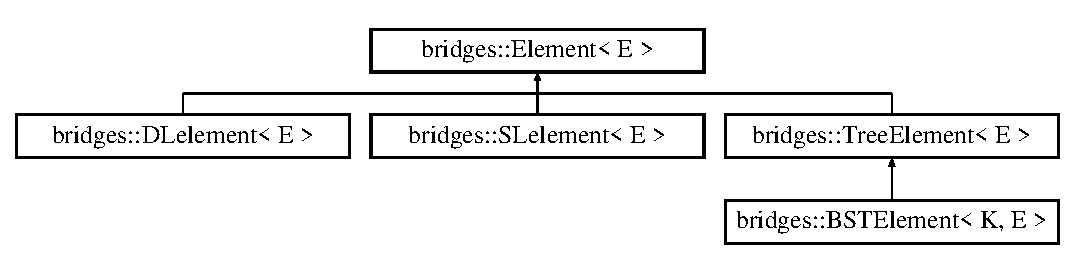
\includegraphics[height=3.000000cm]{classbridges_1_1_element}
\end{center}
\end{figure}
\subsection*{Public Member Functions}
\begin{DoxyCompactItemize}
\item 
\hyperlink{classbridges_1_1_element_ae5eca68c417b51977f258ac6a3d1e9bc}{Element} ()
\item 
\hyperlink{classbridges_1_1_element_af351d4925aa7b5d57effbadd44bb415c}{Element} (const \hyperlink{classbridges_1_1_element}{Element} \&el)
\item 
\hyperlink{classbridges_1_1_element}{Element} \& \hyperlink{classbridges_1_1_element_a5fccf2fed3ae841aff1f8d8bff0bd11b}{operator=} (const \hyperlink{classbridges_1_1_element}{Element} \&el)
\item 
\hyperlink{classbridges_1_1_element_aa4ad8f18cd7d041a8f07701cdb7dfa1a}{Element} (E val)
\item 
\hyperlink{classbridges_1_1_element_a5878b7cb3b9e4abfe9f8d63b22936365}{Element} (string labl, E val)
\item 
\hyperlink{classbridges_1_1_element_a7120a675b75bf30fcbe88c3b6d0a2e30}{$\sim$\+Element} ()
\item 
void \hyperlink{classbridges_1_1_element_a44b88a2d97a96aa6c443334046f425a7}{set\+Visualizer} (\hyperlink{classbridges_1_1_element_visualizer}{Element\+Visualizer} el\+\_\+vis)
\item 
string \hyperlink{classbridges_1_1_element_a2a26b9cd7de3a865f1d95dcc598b5ae3}{get\+Identifier} ()
\item 
\hyperlink{classbridges_1_1_element_visualizer}{Element\+Visualizer} $\ast$ \hyperlink{classbridges_1_1_element_a358f350ae6e33d55c4ac9f9213d0c5bc}{get\+Visualizer} ()
\item 
\hyperlink{classbridges_1_1_link_visualizer}{Link\+Visualizer} $\ast$ \hyperlink{classbridges_1_1_element_a28a5d72ff03d6a66726a2c93ad2a9632}{get\+Link\+Visualizer} (\hyperlink{classbridges_1_1_element}{Element}$<$ E $>$ $\ast$el)
\item 
string \hyperlink{classbridges_1_1_element_a0648a2983f9740f2beec136f9d3a7008}{get\+Representation} ()
\item 
string \hyperlink{classbridges_1_1_element_a506d0f16ebe84cf1351e9d8726b57c14}{get\+Label} ()
\item 
void \hyperlink{classbridges_1_1_element_a49c80a5aa20b0feb6d4f551ac206b51c}{set\+Label} (string label)
\item 
E \hyperlink{classbridges_1_1_element_a9b11b247ebb6ea584a9df414d47a9abc}{get\+Value} ()
\item 
void \hyperlink{classbridges_1_1_element_a54de77e83f615a3c27b46090ea4ba2fb}{set\+Value} (E value)
\end{DoxyCompactItemize}


\subsection{Constructor \& Destructor Documentation}
\hypertarget{classbridges_1_1_element_ae5eca68c417b51977f258ac6a3d1e9bc}{}\index{bridges\+::\+Element@{bridges\+::\+Element}!Element@{Element}}
\index{Element@{Element}!bridges\+::\+Element@{bridges\+::\+Element}}
\subsubsection[{Element}]{\setlength{\rightskip}{0pt plus 5cm}template$<$typename E$>$ {\bf bridges\+::\+Element}$<$ E $>$\+::{\bf Element} (
\begin{DoxyParamCaption}
{}
\end{DoxyParamCaption}
)\hspace{0.3cm}{\ttfamily [inline]}}\label{classbridges_1_1_element_ae5eca68c417b51977f258ac6a3d1e9bc}
\hyperlink{classbridges_1_1_element}{Element} constructor creates an \hyperlink{classbridges_1_1_element_visualizer}{Element\+Visualizer} object sets a unique identifier for the current \hyperlink{classbridges_1_1_element}{Element} normally used from subclasses \hypertarget{classbridges_1_1_element_af351d4925aa7b5d57effbadd44bb415c}{}\index{bridges\+::\+Element@{bridges\+::\+Element}!Element@{Element}}
\index{Element@{Element}!bridges\+::\+Element@{bridges\+::\+Element}}
\subsubsection[{Element}]{\setlength{\rightskip}{0pt plus 5cm}template$<$typename E$>$ {\bf bridges\+::\+Element}$<$ E $>$\+::{\bf Element} (
\begin{DoxyParamCaption}
\item[{const {\bf Element}$<$ E $>$ \&}]{el}
\end{DoxyParamCaption}
)\hspace{0.3cm}{\ttfamily [inline]}}\label{classbridges_1_1_element_af351d4925aa7b5d57effbadd44bb415c}
copy constructor \hypertarget{classbridges_1_1_element_aa4ad8f18cd7d041a8f07701cdb7dfa1a}{}\index{bridges\+::\+Element@{bridges\+::\+Element}!Element@{Element}}
\index{Element@{Element}!bridges\+::\+Element@{bridges\+::\+Element}}
\subsubsection[{Element}]{\setlength{\rightskip}{0pt plus 5cm}template$<$typename E$>$ {\bf bridges\+::\+Element}$<$ E $>$\+::{\bf Element} (
\begin{DoxyParamCaption}
\item[{E}]{val}
\end{DoxyParamCaption}
)\hspace{0.3cm}{\ttfamily [inline]}}\label{classbridges_1_1_element_aa4ad8f18cd7d041a8f07701cdb7dfa1a}
the constructor of \hyperlink{classbridges_1_1_element}{Element} 
\begin{DoxyParams}{Parameters}
{\em val} & will be used to construct \hyperlink{classbridges_1_1_element}{Element} \\
\hline
\end{DoxyParams}
\hypertarget{classbridges_1_1_element_a5878b7cb3b9e4abfe9f8d63b22936365}{}\index{bridges\+::\+Element@{bridges\+::\+Element}!Element@{Element}}
\index{Element@{Element}!bridges\+::\+Element@{bridges\+::\+Element}}
\subsubsection[{Element}]{\setlength{\rightskip}{0pt plus 5cm}template$<$typename E$>$ {\bf bridges\+::\+Element}$<$ E $>$\+::{\bf Element} (
\begin{DoxyParamCaption}
\item[{string}]{labl, }
\item[{E}]{val}
\end{DoxyParamCaption}
)\hspace{0.3cm}{\ttfamily [inline]}}\label{classbridges_1_1_element_a5878b7cb3b9e4abfe9f8d63b22936365}
the constructor of \hyperlink{classbridges_1_1_element}{Element} 
\begin{DoxyParams}{Parameters}
{\em label} & the string that is visible on the \hyperlink{classbridges_1_1_bridges}{Bridges} Visualization \\
\hline
{\em val} & will be used to construct \hyperlink{classbridges_1_1_element}{Element}\textquotesingle{}s data component \\
\hline
\end{DoxyParams}
\hypertarget{classbridges_1_1_element_a7120a675b75bf30fcbe88c3b6d0a2e30}{}\index{bridges\+::\+Element@{bridges\+::\+Element}!````~Element@{$\sim$\+Element}}
\index{````~Element@{$\sim$\+Element}!bridges\+::\+Element@{bridges\+::\+Element}}
\subsubsection[{$\sim$\+Element}]{\setlength{\rightskip}{0pt plus 5cm}template$<$typename E$>$ {\bf bridges\+::\+Element}$<$ E $>$\+::$\sim${\bf Element} (
\begin{DoxyParamCaption}
{}
\end{DoxyParamCaption}
)\hspace{0.3cm}{\ttfamily [inline]}}\label{classbridges_1_1_element_a7120a675b75bf30fcbe88c3b6d0a2e30}
destructor 

\subsection{Member Function Documentation}
\hypertarget{classbridges_1_1_element_a2a26b9cd7de3a865f1d95dcc598b5ae3}{}\index{bridges\+::\+Element@{bridges\+::\+Element}!get\+Identifier@{get\+Identifier}}
\index{get\+Identifier@{get\+Identifier}!bridges\+::\+Element@{bridges\+::\+Element}}
\subsubsection[{get\+Identifier}]{\setlength{\rightskip}{0pt plus 5cm}template$<$typename E$>$ string {\bf bridges\+::\+Element}$<$ E $>$\+::get\+Identifier (
\begin{DoxyParamCaption}
{}
\end{DoxyParamCaption}
)\hspace{0.3cm}{\ttfamily [inline]}}\label{classbridges_1_1_element_a2a26b9cd7de3a865f1d95dcc598b5ae3}
this method returns the element\textquotesingle{}s unique identifier \begin{DoxyReturn}{Returns}
the string identifier 
\end{DoxyReturn}
\hypertarget{classbridges_1_1_element_a506d0f16ebe84cf1351e9d8726b57c14}{}\index{bridges\+::\+Element@{bridges\+::\+Element}!get\+Label@{get\+Label}}
\index{get\+Label@{get\+Label}!bridges\+::\+Element@{bridges\+::\+Element}}
\subsubsection[{get\+Label}]{\setlength{\rightskip}{0pt plus 5cm}template$<$typename E$>$ string {\bf bridges\+::\+Element}$<$ E $>$\+::get\+Label (
\begin{DoxyParamCaption}
{}
\end{DoxyParamCaption}
)\hspace{0.3cm}{\ttfamily [inline]}}\label{classbridges_1_1_element_a506d0f16ebe84cf1351e9d8726b57c14}
This method returns the existing value of the label fields \begin{DoxyReturn}{Returns}
the label of the \hyperlink{classbridges_1_1_element}{Element} that shows up on the \hyperlink{classbridges_1_1_bridges}{Bridges} Visualization 
\end{DoxyReturn}
\hypertarget{classbridges_1_1_element_a28a5d72ff03d6a66726a2c93ad2a9632}{}\index{bridges\+::\+Element@{bridges\+::\+Element}!get\+Link\+Visualizer@{get\+Link\+Visualizer}}
\index{get\+Link\+Visualizer@{get\+Link\+Visualizer}!bridges\+::\+Element@{bridges\+::\+Element}}
\subsubsection[{get\+Link\+Visualizer}]{\setlength{\rightskip}{0pt plus 5cm}template$<$typename E$>$ {\bf Link\+Visualizer}$\ast$ {\bf bridges\+::\+Element}$<$ E $>$\+::get\+Link\+Visualizer (
\begin{DoxyParamCaption}
\item[{{\bf Element}$<$ E $>$ $\ast$}]{el}
\end{DoxyParamCaption}
)\hspace{0.3cm}{\ttfamily [inline]}}\label{classbridges_1_1_element_a28a5d72ff03d6a66726a2c93ad2a9632}
Returns the \hyperlink{classbridges_1_1_element}{Element}\textquotesingle{}s link visualizer object that is linked to element el  \hyperlink{classbridges_1_1_element}{Element} el -- the element terminating the link \begin{DoxyReturn}{Returns}
the link visualizer 
\end{DoxyReturn}
\hypertarget{classbridges_1_1_element_a0648a2983f9740f2beec136f9d3a7008}{}\index{bridges\+::\+Element@{bridges\+::\+Element}!get\+Representation@{get\+Representation}}
\index{get\+Representation@{get\+Representation}!bridges\+::\+Element@{bridges\+::\+Element}}
\subsubsection[{get\+Representation}]{\setlength{\rightskip}{0pt plus 5cm}template$<$typename E$>$ string {\bf bridges\+::\+Element}$<$ E $>$\+::get\+Representation (
\begin{DoxyParamCaption}
{}
\end{DoxyParamCaption}
)\hspace{0.3cm}{\ttfamily [inline]}}\label{classbridges_1_1_element_a0648a2983f9740f2beec136f9d3a7008}
Internal code for getting the properties of the \hyperlink{classbridges_1_1_element}{Element} object. It produces (without the spaces or newlines)\+: \{ \char`\"{}name\char`\"{}\+: \char`\"{}\+Some label\char`\"{}, \char`\"{}other C\+S\+S properties like color\char`\"{}\+: any\+\_\+\+J\+S\+O\+N\+\_\+value \} \begin{DoxyReturn}{Returns}
the encoded J\+S\+O\+N string 
\end{DoxyReturn}
\hypertarget{classbridges_1_1_element_a9b11b247ebb6ea584a9df414d47a9abc}{}\index{bridges\+::\+Element@{bridges\+::\+Element}!get\+Value@{get\+Value}}
\index{get\+Value@{get\+Value}!bridges\+::\+Element@{bridges\+::\+Element}}
\subsubsection[{get\+Value}]{\setlength{\rightskip}{0pt plus 5cm}template$<$typename E$>$ E {\bf bridges\+::\+Element}$<$ E $>$\+::get\+Value (
\begin{DoxyParamCaption}
{}
\end{DoxyParamCaption}
)\hspace{0.3cm}{\ttfamily [inline]}}\label{classbridges_1_1_element_a9b11b247ebb6ea584a9df414d47a9abc}
this method returns the value E for the current \hyperlink{classbridges_1_1_element}{Element} \begin{DoxyReturn}{Returns}
the value 
\end{DoxyReturn}
\hypertarget{classbridges_1_1_element_a358f350ae6e33d55c4ac9f9213d0c5bc}{}\index{bridges\+::\+Element@{bridges\+::\+Element}!get\+Visualizer@{get\+Visualizer}}
\index{get\+Visualizer@{get\+Visualizer}!bridges\+::\+Element@{bridges\+::\+Element}}
\subsubsection[{get\+Visualizer}]{\setlength{\rightskip}{0pt plus 5cm}template$<$typename E$>$ {\bf Element\+Visualizer}$\ast$ {\bf bridges\+::\+Element}$<$ E $>$\+::get\+Visualizer (
\begin{DoxyParamCaption}
{}
\end{DoxyParamCaption}
)\hspace{0.3cm}{\ttfamily [inline]}}\label{classbridges_1_1_element_a358f350ae6e33d55c4ac9f9213d0c5bc}
Returns the \hyperlink{classbridges_1_1_element}{Element}\textquotesingle{}s visualizer object \begin{DoxyReturn}{Returns}
the visualizer 
\end{DoxyReturn}
\hypertarget{classbridges_1_1_element_a5fccf2fed3ae841aff1f8d8bff0bd11b}{}\index{bridges\+::\+Element@{bridges\+::\+Element}!operator=@{operator=}}
\index{operator=@{operator=}!bridges\+::\+Element@{bridges\+::\+Element}}
\subsubsection[{operator=}]{\setlength{\rightskip}{0pt plus 5cm}template$<$typename E$>$ {\bf Element}\& {\bf bridges\+::\+Element}$<$ E $>$\+::operator= (
\begin{DoxyParamCaption}
\item[{const {\bf Element}$<$ E $>$ \&}]{el}
\end{DoxyParamCaption}
)\hspace{0.3cm}{\ttfamily [inline]}}\label{classbridges_1_1_element_a5fccf2fed3ae841aff1f8d8bff0bd11b}
define assignment \hypertarget{classbridges_1_1_element_a49c80a5aa20b0feb6d4f551ac206b51c}{}\index{bridges\+::\+Element@{bridges\+::\+Element}!set\+Label@{set\+Label}}
\index{set\+Label@{set\+Label}!bridges\+::\+Element@{bridges\+::\+Element}}
\subsubsection[{set\+Label}]{\setlength{\rightskip}{0pt plus 5cm}template$<$typename E$>$ void {\bf bridges\+::\+Element}$<$ E $>$\+::set\+Label (
\begin{DoxyParamCaption}
\item[{string}]{label}
\end{DoxyParamCaption}
)\hspace{0.3cm}{\ttfamily [inline]}}\label{classbridges_1_1_element_a49c80a5aa20b0feb6d4f551ac206b51c}
This method sets the label 
\begin{DoxyParams}{Parameters}
{\em label} & the label to set \\
\hline
\end{DoxyParams}
\hypertarget{classbridges_1_1_element_a54de77e83f615a3c27b46090ea4ba2fb}{}\index{bridges\+::\+Element@{bridges\+::\+Element}!set\+Value@{set\+Value}}
\index{set\+Value@{set\+Value}!bridges\+::\+Element@{bridges\+::\+Element}}
\subsubsection[{set\+Value}]{\setlength{\rightskip}{0pt plus 5cm}template$<$typename E$>$ void {\bf bridges\+::\+Element}$<$ E $>$\+::set\+Value (
\begin{DoxyParamCaption}
\item[{E}]{value}
\end{DoxyParamCaption}
)\hspace{0.3cm}{\ttfamily [inline]}}\label{classbridges_1_1_element_a54de77e83f615a3c27b46090ea4ba2fb}
This method sets the value field to the E argument value 
\begin{DoxyParams}{Parameters}
{\em value} & the value to set \\
\hline
\end{DoxyParams}
\hypertarget{classbridges_1_1_element_a44b88a2d97a96aa6c443334046f425a7}{}\index{bridges\+::\+Element@{bridges\+::\+Element}!set\+Visualizer@{set\+Visualizer}}
\index{set\+Visualizer@{set\+Visualizer}!bridges\+::\+Element@{bridges\+::\+Element}}
\subsubsection[{set\+Visualizer}]{\setlength{\rightskip}{0pt plus 5cm}template$<$typename E$>$ void {\bf bridges\+::\+Element}$<$ E $>$\+::set\+Visualizer (
\begin{DoxyParamCaption}
\item[{{\bf Element\+Visualizer}}]{el\+\_\+vis}
\end{DoxyParamCaption}
)\hspace{0.3cm}{\ttfamily [inline]}}\label{classbridges_1_1_element_a44b88a2d97a96aa6c443334046f425a7}
This method sets the visualizer object for the current element object 
\begin{DoxyParams}{Parameters}
{\em visualizer} & the visualizer to set \\
\hline
\end{DoxyParams}


The documentation for this class was generated from the following file\+:\begin{DoxyCompactItemize}
\item 
src/\hyperlink{_element_8h}{Element.\+h}\end{DoxyCompactItemize}

\hypertarget{classbridges_1_1_element_visualizer}{}\section{bridges\+:\+:Element\+Visualizer Class Reference}
\label{classbridges_1_1_element_visualizer}\index{bridges\+::\+Element\+Visualizer@{bridges\+::\+Element\+Visualizer}}


{\ttfamily \#include $<$Element\+Visualizer.\+h$>$}

\subsection*{Public Member Functions}
\begin{DoxyCompactItemize}
\item 
\hyperlink{classbridges_1_1_element_visualizer_a86b6777b9876af6ae828fa121c2fc73e}{Element\+Visualizer} ()
\item 
\hyperlink{classbridges_1_1_element_visualizer_a1717e4bcda460daf907b59a5c17ed5df}{Element\+Visualizer} (string a\+Color)
\item 
\hyperlink{classbridges_1_1_element_visualizer_a175552169fe2dc9343409ccaedc00495}{Element\+Visualizer} (string a\+Color, string a\+Shape)
\item 
\hyperlink{classbridges_1_1_element_visualizer_a6734ec0c1f57982bffbc89e83e4ef9ae}{Element\+Visualizer} (double size)
\item 
\hyperlink{classbridges_1_1_element_visualizer_a698d793a056d4be4ec3681f26d1cb8d9}{Element\+Visualizer} (string a\+Color, string a\+Shape, double opacity, double size)
\item 
\hyperlink{classbridges_1_1_element_visualizer_a8bfb9b2c3749fe435d7d22fe62839243}{Element\+Visualizer} (\hyperlink{classbridges_1_1_element_visualizer}{Element\+Visualizer} \&ev)
\item 
void \hyperlink{classbridges_1_1_element_visualizer_a23889f9093c03ca79a9509312f68d7df}{set\+Size} (double size)
\item 
double \hyperlink{classbridges_1_1_element_visualizer_a00b71f8c783eec23124e925c591b85c0}{get\+Size} ()
\item 
void \hyperlink{classbridges_1_1_element_visualizer_a3ffb0a08204bb86acee0e581c2021c07}{set\+Color} (string a\+Color)
\item 
string \hyperlink{classbridges_1_1_element_visualizer_af33ea5c9fb989673618f90f4059e7e3f}{get\+Color} ()
\item 
void \hyperlink{classbridges_1_1_element_visualizer_a0b40cd56ebfa866cca626b58d172f102}{set\+Shape} (string a\+Shape)
\item 
string \hyperlink{classbridges_1_1_element_visualizer_afebf55de6095e3e23756cc0ce1d57f65}{get\+Shape} ()
\item 
void \hyperlink{classbridges_1_1_element_visualizer_a8f77db4a2774021aec4ab8ea18e50fc9}{set\+Opacity} (double opacity)
\item 
double \hyperlink{classbridges_1_1_element_visualizer_ae806977ebc8ff1c5bce81c90b31902b5}{get\+Opacity} ()
\item 
void \hyperlink{classbridges_1_1_element_visualizer_adcf5ab71a7ead77e8629314aabf9ca90}{set\+Key} (string k)
\item 
unordered\+\_\+map$<$ string, string $>$ \hyperlink{classbridges_1_1_element_visualizer_a0dc2be43a59b42b1ce2d4960a4cc6d59}{get\+Properties} ()
\end{DoxyCompactItemize}


\subsection{Constructor \& Destructor Documentation}
\hypertarget{classbridges_1_1_element_visualizer_a86b6777b9876af6ae828fa121c2fc73e}{}\index{bridges\+::\+Element\+Visualizer@{bridges\+::\+Element\+Visualizer}!Element\+Visualizer@{Element\+Visualizer}}
\index{Element\+Visualizer@{Element\+Visualizer}!bridges\+::\+Element\+Visualizer@{bridges\+::\+Element\+Visualizer}}
\subsubsection[{Element\+Visualizer}]{\setlength{\rightskip}{0pt plus 5cm}bridges\+::\+Element\+Visualizer\+::\+Element\+Visualizer (
\begin{DoxyParamCaption}
{}
\end{DoxyParamCaption}
)\hspace{0.3cm}{\ttfamily [inline]}}\label{classbridges_1_1_element_visualizer_a86b6777b9876af6ae828fa121c2fc73e}
Construct an \hyperlink{classbridges_1_1_element_visualizer}{Element\+Visualizer} with the default visualization settings. Default settings are color = green, opacity = 1.\+0, size = 10.\+0, shape = circle. \hypertarget{classbridges_1_1_element_visualizer_a1717e4bcda460daf907b59a5c17ed5df}{}\index{bridges\+::\+Element\+Visualizer@{bridges\+::\+Element\+Visualizer}!Element\+Visualizer@{Element\+Visualizer}}
\index{Element\+Visualizer@{Element\+Visualizer}!bridges\+::\+Element\+Visualizer@{bridges\+::\+Element\+Visualizer}}
\subsubsection[{Element\+Visualizer}]{\setlength{\rightskip}{0pt plus 5cm}bridges\+::\+Element\+Visualizer\+::\+Element\+Visualizer (
\begin{DoxyParamCaption}
\item[{string}]{a\+Color}
\end{DoxyParamCaption}
)\hspace{0.3cm}{\ttfamily [inline]}}\label{classbridges_1_1_element_visualizer_a1717e4bcda460daf907b59a5c17ed5df}
Construct an \hyperlink{classbridges_1_1_element_visualizer}{Element\+Visualizer} with its color set to \char`\"{}a\+Color\char`\"{}.


\begin{DoxyParams}{Parameters}
{\em a\+Color} & the string that represents one of the \hyperlink{classbridges_1_1_bridges}{Bridges} colors. \\
\hline
\end{DoxyParams}
\hypertarget{classbridges_1_1_element_visualizer_a175552169fe2dc9343409ccaedc00495}{}\index{bridges\+::\+Element\+Visualizer@{bridges\+::\+Element\+Visualizer}!Element\+Visualizer@{Element\+Visualizer}}
\index{Element\+Visualizer@{Element\+Visualizer}!bridges\+::\+Element\+Visualizer@{bridges\+::\+Element\+Visualizer}}
\subsubsection[{Element\+Visualizer}]{\setlength{\rightskip}{0pt plus 5cm}bridges\+::\+Element\+Visualizer\+::\+Element\+Visualizer (
\begin{DoxyParamCaption}
\item[{string}]{a\+Color, }
\item[{string}]{a\+Shape}
\end{DoxyParamCaption}
)\hspace{0.3cm}{\ttfamily [inline]}}\label{classbridges_1_1_element_visualizer_a175552169fe2dc9343409ccaedc00495}
Construct an \hyperlink{classbridges_1_1_element_visualizer}{Element\+Visualizer} with its color set to \char`\"{}a\+Color\char`\"{} and shape set to \char`\"{}a\+Shape\char`\"{}.


\begin{DoxyParams}{Parameters}
{\em a\+Color} & the string that represents one of the \hyperlink{classbridges_1_1_bridges}{Bridges} colors. \\
\hline
{\em a\+Shape} & the string that represents one of the \hyperlink{classbridges_1_1_bridges}{Bridges} shapes \\
\hline
\end{DoxyParams}
\hypertarget{classbridges_1_1_element_visualizer_a6734ec0c1f57982bffbc89e83e4ef9ae}{}\index{bridges\+::\+Element\+Visualizer@{bridges\+::\+Element\+Visualizer}!Element\+Visualizer@{Element\+Visualizer}}
\index{Element\+Visualizer@{Element\+Visualizer}!bridges\+::\+Element\+Visualizer@{bridges\+::\+Element\+Visualizer}}
\subsubsection[{Element\+Visualizer}]{\setlength{\rightskip}{0pt plus 5cm}bridges\+::\+Element\+Visualizer\+::\+Element\+Visualizer (
\begin{DoxyParamCaption}
\item[{double}]{size}
\end{DoxyParamCaption}
)\hspace{0.3cm}{\ttfamily [inline]}}\label{classbridges_1_1_element_visualizer_a6734ec0c1f57982bffbc89e83e4ef9ae}
Construct an \hyperlink{classbridges_1_1_element_visualizer}{Element\+Visualizer} with its size set to \char`\"{}size\char`\"{}.


\begin{DoxyParams}{Parameters}
{\em size} & \+: the double that represents the size in pixels of the \hyperlink{classbridges_1_1_element}{Element} on the \hyperlink{classbridges_1_1_bridges}{Bridges} Visualization \\
\hline
\end{DoxyParams}
\hypertarget{classbridges_1_1_element_visualizer_a698d793a056d4be4ec3681f26d1cb8d9}{}\index{bridges\+::\+Element\+Visualizer@{bridges\+::\+Element\+Visualizer}!Element\+Visualizer@{Element\+Visualizer}}
\index{Element\+Visualizer@{Element\+Visualizer}!bridges\+::\+Element\+Visualizer@{bridges\+::\+Element\+Visualizer}}
\subsubsection[{Element\+Visualizer}]{\setlength{\rightskip}{0pt plus 5cm}bridges\+::\+Element\+Visualizer\+::\+Element\+Visualizer (
\begin{DoxyParamCaption}
\item[{string}]{a\+Color, }
\item[{string}]{a\+Shape, }
\item[{double}]{opacity, }
\item[{double}]{size}
\end{DoxyParamCaption}
)\hspace{0.3cm}{\ttfamily [inline]}}\label{classbridges_1_1_element_visualizer_a698d793a056d4be4ec3681f26d1cb8d9}
Construct an \hyperlink{classbridges_1_1_element_visualizer}{Element\+Visualizer} with its color set to \char`\"{}a\+Color\char`\"{}, its shape set to \char`\"{}a\+Shape\char`\"{}, its opacity set to \char`\"{}opacity\char`\"{} and size set to \char`\"{}size\char`\"{}. 
\begin{DoxyParams}{Parameters}
{\em a\+Color} & the string that represents one of the \hyperlink{classbridges_1_1_bridges}{Bridges} colors. \\
\hline
{\em a\+Shape} & the string that represents one of the \hyperlink{classbridges_1_1_bridges}{Bridges} shapes \\
\hline
{\em opacity} & a double between 0 and 1 representing how transparent the node should be on the \hyperlink{classbridges_1_1_bridges}{Bridges} Visualization. 0 for invisible, 1 for fully visible, a decimal between 0 and 1 for varying transparency. \\
\hline
{\em size} & the double that represents the size of the \hyperlink{classbridges_1_1_element}{Element} on the \hyperlink{classbridges_1_1_bridges}{Bridges} Visualization \\
\hline
\end{DoxyParams}
\hypertarget{classbridges_1_1_element_visualizer_a8bfb9b2c3749fe435d7d22fe62839243}{}\index{bridges\+::\+Element\+Visualizer@{bridges\+::\+Element\+Visualizer}!Element\+Visualizer@{Element\+Visualizer}}
\index{Element\+Visualizer@{Element\+Visualizer}!bridges\+::\+Element\+Visualizer@{bridges\+::\+Element\+Visualizer}}
\subsubsection[{Element\+Visualizer}]{\setlength{\rightskip}{0pt plus 5cm}bridges\+::\+Element\+Visualizer\+::\+Element\+Visualizer (
\begin{DoxyParamCaption}
\item[{{\bf Element\+Visualizer} \&}]{ev}
\end{DoxyParamCaption}
)\hspace{0.3cm}{\ttfamily [inline]}}\label{classbridges_1_1_element_visualizer_a8bfb9b2c3749fe435d7d22fe62839243}
Construct a new \hyperlink{classbridges_1_1_element_visualizer}{Element\+Visualizer} with the same color, shape, opacity, and size as \char`\"{}v\char`\"{}


\begin{DoxyParams}{Parameters}
{\em v} & the \hyperlink{classbridges_1_1_element_visualizer}{Element\+Visualizer} whose settings you want to copy. \\
\hline
\end{DoxyParams}


\subsection{Member Function Documentation}
\hypertarget{classbridges_1_1_element_visualizer_af33ea5c9fb989673618f90f4059e7e3f}{}\index{bridges\+::\+Element\+Visualizer@{bridges\+::\+Element\+Visualizer}!get\+Color@{get\+Color}}
\index{get\+Color@{get\+Color}!bridges\+::\+Element\+Visualizer@{bridges\+::\+Element\+Visualizer}}
\subsubsection[{get\+Color}]{\setlength{\rightskip}{0pt plus 5cm}string bridges\+::\+Element\+Visualizer\+::get\+Color (
\begin{DoxyParamCaption}
{}
\end{DoxyParamCaption}
)\hspace{0.3cm}{\ttfamily [inline]}}\label{classbridges_1_1_element_visualizer_af33ea5c9fb989673618f90f4059e7e3f}
Get the color of the \hyperlink{classbridges_1_1_element}{Element} in the \hyperlink{classbridges_1_1_bridges}{Bridges} Visualization \begin{DoxyReturn}{Returns}
the string reprsenting the color of the \hyperlink{classbridges_1_1_element}{Element} in the \hyperlink{classbridges_1_1_bridges}{Bridges} Visualization 
\end{DoxyReturn}
\hypertarget{classbridges_1_1_element_visualizer_ae806977ebc8ff1c5bce81c90b31902b5}{}\index{bridges\+::\+Element\+Visualizer@{bridges\+::\+Element\+Visualizer}!get\+Opacity@{get\+Opacity}}
\index{get\+Opacity@{get\+Opacity}!bridges\+::\+Element\+Visualizer@{bridges\+::\+Element\+Visualizer}}
\subsubsection[{get\+Opacity}]{\setlength{\rightskip}{0pt plus 5cm}double bridges\+::\+Element\+Visualizer\+::get\+Opacity (
\begin{DoxyParamCaption}
{}
\end{DoxyParamCaption}
)\hspace{0.3cm}{\ttfamily [inline]}}\label{classbridges_1_1_element_visualizer_ae806977ebc8ff1c5bce81c90b31902b5}
Get the opacity of the \hyperlink{classbridges_1_1_element}{Element} in the \hyperlink{classbridges_1_1_bridges}{Bridges} Visualization \begin{DoxyReturn}{Returns}
the opacity value 
\end{DoxyReturn}
\hypertarget{classbridges_1_1_element_visualizer_a0dc2be43a59b42b1ce2d4960a4cc6d59}{}\index{bridges\+::\+Element\+Visualizer@{bridges\+::\+Element\+Visualizer}!get\+Properties@{get\+Properties}}
\index{get\+Properties@{get\+Properties}!bridges\+::\+Element\+Visualizer@{bridges\+::\+Element\+Visualizer}}
\subsubsection[{get\+Properties}]{\setlength{\rightskip}{0pt plus 5cm}unordered\+\_\+map$<$string, string$>$ bridges\+::\+Element\+Visualizer\+::get\+Properties (
\begin{DoxyParamCaption}
{}
\end{DoxyParamCaption}
)\hspace{0.3cm}{\ttfamily [inline]}}\label{classbridges_1_1_element_visualizer_a0dc2be43a59b42b1ce2d4960a4cc6d59}
This method returns the properties map

\begin{DoxyReturn}{Returns}
the properties map 
\end{DoxyReturn}
\hypertarget{classbridges_1_1_element_visualizer_afebf55de6095e3e23756cc0ce1d57f65}{}\index{bridges\+::\+Element\+Visualizer@{bridges\+::\+Element\+Visualizer}!get\+Shape@{get\+Shape}}
\index{get\+Shape@{get\+Shape}!bridges\+::\+Element\+Visualizer@{bridges\+::\+Element\+Visualizer}}
\subsubsection[{get\+Shape}]{\setlength{\rightskip}{0pt plus 5cm}string bridges\+::\+Element\+Visualizer\+::get\+Shape (
\begin{DoxyParamCaption}
{}
\end{DoxyParamCaption}
)\hspace{0.3cm}{\ttfamily [inline]}}\label{classbridges_1_1_element_visualizer_afebf55de6095e3e23756cc0ce1d57f65}
Get the shape of the \hyperlink{classbridges_1_1_element}{Element} in the \hyperlink{classbridges_1_1_bridges}{Bridges} Visualization. \begin{DoxyReturn}{Returns}
the string that represents the \hyperlink{classbridges_1_1_element}{Element}\textquotesingle{}s shape in the \hyperlink{classbridges_1_1_bridges}{Bridges} Visualization. 
\end{DoxyReturn}
\hypertarget{classbridges_1_1_element_visualizer_a00b71f8c783eec23124e925c591b85c0}{}\index{bridges\+::\+Element\+Visualizer@{bridges\+::\+Element\+Visualizer}!get\+Size@{get\+Size}}
\index{get\+Size@{get\+Size}!bridges\+::\+Element\+Visualizer@{bridges\+::\+Element\+Visualizer}}
\subsubsection[{get\+Size}]{\setlength{\rightskip}{0pt plus 5cm}double bridges\+::\+Element\+Visualizer\+::get\+Size (
\begin{DoxyParamCaption}
{}
\end{DoxyParamCaption}
)\hspace{0.3cm}{\ttfamily [inline]}}\label{classbridges_1_1_element_visualizer_a00b71f8c783eec23124e925c591b85c0}
Get the size of the \hyperlink{classbridges_1_1_element}{Element} in the \hyperlink{classbridges_1_1_bridges}{Bridges} Visualiation

\begin{DoxyReturn}{Returns}
the size in pixels of the \hyperlink{classbridges_1_1_element}{Element} in the \hyperlink{classbridges_1_1_bridges}{Bridges} Visualization 
\end{DoxyReturn}
\hypertarget{classbridges_1_1_element_visualizer_a3ffb0a08204bb86acee0e581c2021c07}{}\index{bridges\+::\+Element\+Visualizer@{bridges\+::\+Element\+Visualizer}!set\+Color@{set\+Color}}
\index{set\+Color@{set\+Color}!bridges\+::\+Element\+Visualizer@{bridges\+::\+Element\+Visualizer}}
\subsubsection[{set\+Color}]{\setlength{\rightskip}{0pt plus 5cm}void bridges\+::\+Element\+Visualizer\+::set\+Color (
\begin{DoxyParamCaption}
\item[{string}]{a\+Color}
\end{DoxyParamCaption}
)\hspace{0.3cm}{\ttfamily [inline]}}\label{classbridges_1_1_element_visualizer_a3ffb0a08204bb86acee0e581c2021c07}
Set the color of the \hyperlink{classbridges_1_1_element}{Element} in the \hyperlink{classbridges_1_1_bridges}{Bridges} Visualization to \char`\"{}a\+Color\char`\"{}. 
\begin{DoxyParams}{Parameters}
{\em a\+Color} & the string reprsenting the color of the \hyperlink{classbridges_1_1_element}{Element} in the \hyperlink{classbridges_1_1_bridges}{Bridges} Visualization \\
\hline
\end{DoxyParams}
\hypertarget{classbridges_1_1_element_visualizer_adcf5ab71a7ead77e8629314aabf9ca90}{}\index{bridges\+::\+Element\+Visualizer@{bridges\+::\+Element\+Visualizer}!set\+Key@{set\+Key}}
\index{set\+Key@{set\+Key}!bridges\+::\+Element\+Visualizer@{bridges\+::\+Element\+Visualizer}}
\subsubsection[{set\+Key}]{\setlength{\rightskip}{0pt plus 5cm}void bridges\+::\+Element\+Visualizer\+::set\+Key (
\begin{DoxyParamCaption}
\item[{string}]{k}
\end{DoxyParamCaption}
)\hspace{0.3cm}{\ttfamily [inline]}}\label{classbridges_1_1_element_visualizer_adcf5ab71a7ead77e8629314aabf9ca90}
Sets the key value attributed of the \hyperlink{classbridges_1_1_element}{Element} used by search structures -\/ binary search trees, A\+V\+L trees, etc.


\begin{DoxyParams}{Parameters}
{\em key} & is any orderable value -\/ int, float, string \\
\hline
\end{DoxyParams}
\hypertarget{classbridges_1_1_element_visualizer_a8f77db4a2774021aec4ab8ea18e50fc9}{}\index{bridges\+::\+Element\+Visualizer@{bridges\+::\+Element\+Visualizer}!set\+Opacity@{set\+Opacity}}
\index{set\+Opacity@{set\+Opacity}!bridges\+::\+Element\+Visualizer@{bridges\+::\+Element\+Visualizer}}
\subsubsection[{set\+Opacity}]{\setlength{\rightskip}{0pt plus 5cm}void bridges\+::\+Element\+Visualizer\+::set\+Opacity (
\begin{DoxyParamCaption}
\item[{double}]{opacity}
\end{DoxyParamCaption}
)\hspace{0.3cm}{\ttfamily [inline]}}\label{classbridges_1_1_element_visualizer_a8f77db4a2774021aec4ab8ea18e50fc9}
Sets the opacity of the \hyperlink{classbridges_1_1_element}{Element} in the \hyperlink{classbridges_1_1_bridges}{Bridges} Visualization


\begin{DoxyParams}{Parameters}
{\em opacity} & a double value between 0.\+0(fully opaque) and 1 (fully transparent representing how \\
\hline
\end{DoxyParams}
\hypertarget{classbridges_1_1_element_visualizer_a0b40cd56ebfa866cca626b58d172f102}{}\index{bridges\+::\+Element\+Visualizer@{bridges\+::\+Element\+Visualizer}!set\+Shape@{set\+Shape}}
\index{set\+Shape@{set\+Shape}!bridges\+::\+Element\+Visualizer@{bridges\+::\+Element\+Visualizer}}
\subsubsection[{set\+Shape}]{\setlength{\rightskip}{0pt plus 5cm}void bridges\+::\+Element\+Visualizer\+::set\+Shape (
\begin{DoxyParamCaption}
\item[{string}]{a\+Shape}
\end{DoxyParamCaption}
)\hspace{0.3cm}{\ttfamily [inline]}}\label{classbridges_1_1_element_visualizer_a0b40cd56ebfa866cca626b58d172f102}
Sets the shape of the \hyperlink{classbridges_1_1_element}{Element} in the \hyperlink{classbridges_1_1_bridges}{Bridges} Visualization


\begin{DoxyParams}{Parameters}
{\em a\+Shape} & the string representing the shape of the \hyperlink{classbridges_1_1_element}{Element} in the \hyperlink{classbridges_1_1_bridges}{Bridges} Visualization \\
\hline
\end{DoxyParams}
\hypertarget{classbridges_1_1_element_visualizer_a23889f9093c03ca79a9509312f68d7df}{}\index{bridges\+::\+Element\+Visualizer@{bridges\+::\+Element\+Visualizer}!set\+Size@{set\+Size}}
\index{set\+Size@{set\+Size}!bridges\+::\+Element\+Visualizer@{bridges\+::\+Element\+Visualizer}}
\subsubsection[{set\+Size}]{\setlength{\rightskip}{0pt plus 5cm}void bridges\+::\+Element\+Visualizer\+::set\+Size (
\begin{DoxyParamCaption}
\item[{double}]{size}
\end{DoxyParamCaption}
)\hspace{0.3cm}{\ttfamily [inline]}}\label{classbridges_1_1_element_visualizer_a23889f9093c03ca79a9509312f68d7df}
Set the size of the \hyperlink{classbridges_1_1_element}{Element} in the Bridge Visualization in pixels


\begin{DoxyParams}{Parameters}
{\em size} & the pixel size of the \hyperlink{classbridges_1_1_element}{Element} in the \hyperlink{classbridges_1_1_bridges}{Bridges} Visualization \\
\hline
\end{DoxyParams}


The documentation for this class was generated from the following file\+:\begin{DoxyCompactItemize}
\item 
src/\hyperlink{_element_visualizer_8h}{Element\+Visualizer.\+h}\end{DoxyCompactItemize}

\hypertarget{classbridges_1_1_graph_adj_list}{}\section{bridges\+:\+:Graph\+Adj\+List$<$ Key, E $>$ Class Template Reference}
\label{classbridges_1_1_graph_adj_list}\index{bridges\+::\+Graph\+Adj\+List$<$ Key, E $>$@{bridges\+::\+Graph\+Adj\+List$<$ Key, E $>$}}


{\ttfamily \#include $<$Graph\+Adj\+List.\+h$>$}

\subsection*{Public Member Functions}
\begin{DoxyCompactItemize}
\item 
\hyperlink{classbridges_1_1_graph_adj_list_a0a185744acc43305f73a8db0e3bbb7e2}{Graph\+Adj\+List} ()
\item 
\hyperlink{classbridges_1_1_graph_adj_list_ac9b898cd9df35ba09b2eeb6f085e3818}{$\sim$\+Graph\+Adj\+List} ()
\item 
void \hyperlink{classbridges_1_1_graph_adj_list_a813758981e1c64b91450f4026c8e8700}{add\+Vertex} (Key k, E e)
\item 
void \hyperlink{classbridges_1_1_graph_adj_list_a3085d848a5e6ea9c5292e804e2ae80b8}{add\+Edge} (Key src, Key dest, int weight)
\item 
unordered\+\_\+map$<$ Key, \hyperlink{classbridges_1_1_element}{Element}$<$ E $>$ $>$ $\ast$ \hyperlink{classbridges_1_1_graph_adj_list_a07ac6ad2cb0aebab37103de72e2e6719}{get\+Vertices} ()
\item 
unordered\+\_\+map$<$ Key, \hyperlink{classbridges_1_1_s_lelement}{S\+Lelement}$<$ \hyperlink{classbridges_1_1_edge}{Edge}$<$ Key $>$ $>$ $\ast$ $>$ $\ast$ \hyperlink{classbridges_1_1_graph_adj_list_a72f55641dabb692491639451c026496f}{get\+Adjacency\+List} ()
\item 
\hyperlink{classbridges_1_1_s_lelement}{S\+Lelement}$<$ \hyperlink{classbridges_1_1_edge}{Edge}$<$ Key $>$ $>$ $\ast$ \hyperlink{classbridges_1_1_graph_adj_list_a4246f696bdec73aa2c4bdbcce5f66adf}{get\+Adjacency\+List} (Key vertex)
\end{DoxyCompactItemize}


\subsection{Constructor \& Destructor Documentation}
\hypertarget{classbridges_1_1_graph_adj_list_a0a185744acc43305f73a8db0e3bbb7e2}{}\index{bridges\+::\+Graph\+Adj\+List@{bridges\+::\+Graph\+Adj\+List}!Graph\+Adj\+List@{Graph\+Adj\+List}}
\index{Graph\+Adj\+List@{Graph\+Adj\+List}!bridges\+::\+Graph\+Adj\+List@{bridges\+::\+Graph\+Adj\+List}}
\subsubsection[{Graph\+Adj\+List}]{\setlength{\rightskip}{0pt plus 5cm}template$<$typename Key, typename E$>$ {\bf bridges\+::\+Graph\+Adj\+List}$<$ Key, E $>$\+::{\bf Graph\+Adj\+List} (
\begin{DoxyParamCaption}
{}
\end{DoxyParamCaption}
)\hspace{0.3cm}{\ttfamily [inline]}}\label{classbridges_1_1_graph_adj_list_a0a185744acc43305f73a8db0e3bbb7e2}
Constructor \hypertarget{classbridges_1_1_graph_adj_list_ac9b898cd9df35ba09b2eeb6f085e3818}{}\index{bridges\+::\+Graph\+Adj\+List@{bridges\+::\+Graph\+Adj\+List}!````~Graph\+Adj\+List@{$\sim$\+Graph\+Adj\+List}}
\index{````~Graph\+Adj\+List@{$\sim$\+Graph\+Adj\+List}!bridges\+::\+Graph\+Adj\+List@{bridges\+::\+Graph\+Adj\+List}}
\subsubsection[{$\sim$\+Graph\+Adj\+List}]{\setlength{\rightskip}{0pt plus 5cm}template$<$typename Key, typename E$>$ {\bf bridges\+::\+Graph\+Adj\+List}$<$ Key, E $>$\+::$\sim${\bf Graph\+Adj\+List} (
\begin{DoxyParamCaption}
{}
\end{DoxyParamCaption}
)\hspace{0.3cm}{\ttfamily [inline]}}\label{classbridges_1_1_graph_adj_list_ac9b898cd9df35ba09b2eeb6f085e3818}


\subsection{Member Function Documentation}
\hypertarget{classbridges_1_1_graph_adj_list_a3085d848a5e6ea9c5292e804e2ae80b8}{}\index{bridges\+::\+Graph\+Adj\+List@{bridges\+::\+Graph\+Adj\+List}!add\+Edge@{add\+Edge}}
\index{add\+Edge@{add\+Edge}!bridges\+::\+Graph\+Adj\+List@{bridges\+::\+Graph\+Adj\+List}}
\subsubsection[{add\+Edge}]{\setlength{\rightskip}{0pt plus 5cm}template$<$typename Key, typename E$>$ void {\bf bridges\+::\+Graph\+Adj\+List}$<$ Key, E $>$\+::add\+Edge (
\begin{DoxyParamCaption}
\item[{Key}]{src, }
\item[{Key}]{dest, }
\item[{int}]{weight}
\end{DoxyParamCaption}
)\hspace{0.3cm}{\ttfamily [inline]}}\label{classbridges_1_1_graph_adj_list_a3085d848a5e6ea9c5292e804e2ae80b8}
Adds a new edge to the graph, initializes the adjacency list; user is responsible for checking if the vertex already exists. This method will replace the value for this key


\begin{DoxyParams}{Parameters}
{\em src} & -\/ source vertex of edge \\
\hline
{\em dest} & -\/ destination vertex of edge \\
\hline
\end{DoxyParams}
\begin{DoxyReturn}{Returns}
none 
\end{DoxyReturn}
\hypertarget{classbridges_1_1_graph_adj_list_a813758981e1c64b91450f4026c8e8700}{}\index{bridges\+::\+Graph\+Adj\+List@{bridges\+::\+Graph\+Adj\+List}!add\+Vertex@{add\+Vertex}}
\index{add\+Vertex@{add\+Vertex}!bridges\+::\+Graph\+Adj\+List@{bridges\+::\+Graph\+Adj\+List}}
\subsubsection[{add\+Vertex}]{\setlength{\rightskip}{0pt plus 5cm}template$<$typename Key, typename E$>$ void {\bf bridges\+::\+Graph\+Adj\+List}$<$ Key, E $>$\+::add\+Vertex (
\begin{DoxyParamCaption}
\item[{Key}]{k, }
\item[{E}]{e}
\end{DoxyParamCaption}
)\hspace{0.3cm}{\ttfamily [inline]}}\label{classbridges_1_1_graph_adj_list_a813758981e1c64b91450f4026c8e8700}
Adds a new vertex to the graph, initializes the adjacency list; user is responsible for checking if the vertex already exists. This method will replace the value for this key


\begin{DoxyParams}{Parameters}
{\em Key} & -\/ vertex key value \\
\hline
\end{DoxyParams}
\begin{DoxyReturn}{Returns}
none 
\end{DoxyReturn}
\hypertarget{classbridges_1_1_graph_adj_list_a72f55641dabb692491639451c026496f}{}\index{bridges\+::\+Graph\+Adj\+List@{bridges\+::\+Graph\+Adj\+List}!get\+Adjacency\+List@{get\+Adjacency\+List}}
\index{get\+Adjacency\+List@{get\+Adjacency\+List}!bridges\+::\+Graph\+Adj\+List@{bridges\+::\+Graph\+Adj\+List}}
\subsubsection[{get\+Adjacency\+List}]{\setlength{\rightskip}{0pt plus 5cm}template$<$typename Key, typename E$>$ unordered\+\_\+map$<$Key, {\bf S\+Lelement}$<${\bf Edge}$<$Key$>$ $>$$\ast$ $>$$\ast$ {\bf bridges\+::\+Graph\+Adj\+List}$<$ Key, E $>$\+::get\+Adjacency\+List (
\begin{DoxyParamCaption}
{}
\end{DoxyParamCaption}
)\hspace{0.3cm}{\ttfamily [inline]}}\label{classbridges_1_1_graph_adj_list_a72f55641dabb692491639451c026496f}
Gets the adjacency list (of type S\+Lelement$<$\+Edge$>$ $\ast$)

\begin{DoxyReturn}{Returns}
-\/ the graph\textquotesingle{}s adjacency lists 
\end{DoxyReturn}
\hypertarget{classbridges_1_1_graph_adj_list_a4246f696bdec73aa2c4bdbcce5f66adf}{}\index{bridges\+::\+Graph\+Adj\+List@{bridges\+::\+Graph\+Adj\+List}!get\+Adjacency\+List@{get\+Adjacency\+List}}
\index{get\+Adjacency\+List@{get\+Adjacency\+List}!bridges\+::\+Graph\+Adj\+List@{bridges\+::\+Graph\+Adj\+List}}
\subsubsection[{get\+Adjacency\+List}]{\setlength{\rightskip}{0pt plus 5cm}template$<$typename Key, typename E$>$ {\bf S\+Lelement}$<${\bf Edge}$<$Key$>$ $>$$\ast$ {\bf bridges\+::\+Graph\+Adj\+List}$<$ Key, E $>$\+::get\+Adjacency\+List (
\begin{DoxyParamCaption}
\item[{Key}]{vertex}
\end{DoxyParamCaption}
)\hspace{0.3cm}{\ttfamily [inline]}}\label{classbridges_1_1_graph_adj_list_a4246f696bdec73aa2c4bdbcce5f66adf}
Gets the adjacency list (of type S\+Lelement$<$\+Edge$>$ $\ast$ of a vertex)


\begin{DoxyParams}{Parameters}
{\em -\/} & vertex key\\
\hline
\end{DoxyParams}
\begin{DoxyReturn}{Returns}
-\/ the graph\textquotesingle{}s adjacency list corresponding to this vertex 
\end{DoxyReturn}
\hypertarget{classbridges_1_1_graph_adj_list_a07ac6ad2cb0aebab37103de72e2e6719}{}\index{bridges\+::\+Graph\+Adj\+List@{bridges\+::\+Graph\+Adj\+List}!get\+Vertices@{get\+Vertices}}
\index{get\+Vertices@{get\+Vertices}!bridges\+::\+Graph\+Adj\+List@{bridges\+::\+Graph\+Adj\+List}}
\subsubsection[{get\+Vertices}]{\setlength{\rightskip}{0pt plus 5cm}template$<$typename Key, typename E$>$ unordered\+\_\+map$<$Key, {\bf Element}$<$E$>$ $>$$\ast$ {\bf bridges\+::\+Graph\+Adj\+List}$<$ Key, E $>$\+::get\+Vertices (
\begin{DoxyParamCaption}
{}
\end{DoxyParamCaption}
)\hspace{0.3cm}{\ttfamily [inline]}}\label{classbridges_1_1_graph_adj_list_a07ac6ad2cb0aebab37103de72e2e6719}
This method returns the graph nodes

\begin{DoxyReturn}{Returns}
-- vertices held in an unordered map 
\end{DoxyReturn}


The documentation for this class was generated from the following file\+:\begin{DoxyCompactItemize}
\item 
src/\hyperlink{_graph_adj_list_8h}{Graph\+Adj\+List.\+h}\end{DoxyCompactItemize}

\hypertarget{classbridges_1_1_graph_adj_matrix}{}\section{bridges\+:\+:Graph\+Adj\+Matrix$<$ Key, E $>$ Class Template Reference}
\label{classbridges_1_1_graph_adj_matrix}\index{bridges\+::\+Graph\+Adj\+Matrix$<$ Key, E $>$@{bridges\+::\+Graph\+Adj\+Matrix$<$ Key, E $>$}}


{\ttfamily \#include $<$Graph\+Adj\+Matrix.\+h$>$}

\subsection*{Public Member Functions}
\begin{DoxyCompactItemize}
\item 
\hyperlink{classbridges_1_1_graph_adj_matrix_a3c6caf98cf52a41cc446115967571975}{Graph\+Adj\+Matrix} ()
\begin{DoxyCompactList}\small\item\em Constructor. \end{DoxyCompactList}\item 
void \hyperlink{classbridges_1_1_graph_adj_matrix_ade848b5e4fc39bbc3d78f86807f12061}{add\+Vertex} (Key k, E e)
\item 
void \hyperlink{classbridges_1_1_graph_adj_matrix_ad07f73bae1314d5dc2403bb7ebfc9aab}{add\+Edge} (Key src, Key dest, int weight)
\item 
unordered\+\_\+map$<$ Key, unordered\+\_\+map$<$ Key, double $>$ $>$ $\ast$ \hyperlink{classbridges_1_1_graph_adj_matrix_a3407ab17167b1148e963a4aa687ac1a5}{get\+Matrix} ()
\item 
unordered\+\_\+map$<$ Key, \hyperlink{classbridges_1_1_element}{Element}$<$ E $>$ $>$ $\ast$ \hyperlink{classbridges_1_1_graph_adj_matrix_a992b4773b79ccd97716f20f88a14e444}{get\+Vertices} ()
\end{DoxyCompactItemize}


\subsection{Constructor \& Destructor Documentation}
\hypertarget{classbridges_1_1_graph_adj_matrix_a3c6caf98cf52a41cc446115967571975}{}\index{bridges\+::\+Graph\+Adj\+Matrix@{bridges\+::\+Graph\+Adj\+Matrix}!Graph\+Adj\+Matrix@{Graph\+Adj\+Matrix}}
\index{Graph\+Adj\+Matrix@{Graph\+Adj\+Matrix}!bridges\+::\+Graph\+Adj\+Matrix@{bridges\+::\+Graph\+Adj\+Matrix}}
\subsubsection[{Graph\+Adj\+Matrix}]{\setlength{\rightskip}{0pt plus 5cm}template$<$typename Key, typename E$>$ {\bf bridges\+::\+Graph\+Adj\+Matrix}$<$ Key, E $>$\+::{\bf Graph\+Adj\+Matrix} (
\begin{DoxyParamCaption}
{}
\end{DoxyParamCaption}
)\hspace{0.3cm}{\ttfamily [inline]}}\label{classbridges_1_1_graph_adj_matrix_a3c6caf98cf52a41cc446115967571975}


Constructor. 



\subsection{Member Function Documentation}
\hypertarget{classbridges_1_1_graph_adj_matrix_ad07f73bae1314d5dc2403bb7ebfc9aab}{}\index{bridges\+::\+Graph\+Adj\+Matrix@{bridges\+::\+Graph\+Adj\+Matrix}!add\+Edge@{add\+Edge}}
\index{add\+Edge@{add\+Edge}!bridges\+::\+Graph\+Adj\+Matrix@{bridges\+::\+Graph\+Adj\+Matrix}}
\subsubsection[{add\+Edge}]{\setlength{\rightskip}{0pt plus 5cm}template$<$typename Key, typename E$>$ void {\bf bridges\+::\+Graph\+Adj\+Matrix}$<$ Key, E $>$\+::add\+Edge (
\begin{DoxyParamCaption}
\item[{Key}]{src, }
\item[{Key}]{dest, }
\item[{int}]{weight}
\end{DoxyParamCaption}
)\hspace{0.3cm}{\ttfamily [inline]}}\label{classbridges_1_1_graph_adj_matrix_ad07f73bae1314d5dc2403bb7ebfc9aab}
Adds a new edge to the graph, user is responsible for checking if the edge already exists. This method will replace the value for this key, otherwise


\begin{DoxyParams}{Parameters}
{\em src} & -\/ source vertex of edge \\
\hline
{\em dest} & -\/ destination vertex of edge \\
\hline
\end{DoxyParams}
\begin{DoxyReturn}{Returns}
none 
\end{DoxyReturn}
\hypertarget{classbridges_1_1_graph_adj_matrix_ade848b5e4fc39bbc3d78f86807f12061}{}\index{bridges\+::\+Graph\+Adj\+Matrix@{bridges\+::\+Graph\+Adj\+Matrix}!add\+Vertex@{add\+Vertex}}
\index{add\+Vertex@{add\+Vertex}!bridges\+::\+Graph\+Adj\+Matrix@{bridges\+::\+Graph\+Adj\+Matrix}}
\subsubsection[{add\+Vertex}]{\setlength{\rightskip}{0pt plus 5cm}template$<$typename Key, typename E$>$ void {\bf bridges\+::\+Graph\+Adj\+Matrix}$<$ Key, E $>$\+::add\+Vertex (
\begin{DoxyParamCaption}
\item[{Key}]{k, }
\item[{E}]{e}
\end{DoxyParamCaption}
)\hspace{0.3cm}{\ttfamily [inline]}}\label{classbridges_1_1_graph_adj_matrix_ade848b5e4fc39bbc3d78f86807f12061}
Adds a new vertex to the graph, setts the edge to itself to be exists. This method will replace the value for this key


\begin{DoxyParams}{Parameters}
{\em Key} & -\/ vertex key value \\
\hline
\end{DoxyParams}
\begin{DoxyReturn}{Returns}
none 
\end{DoxyReturn}
\hypertarget{classbridges_1_1_graph_adj_matrix_a3407ab17167b1148e963a4aa687ac1a5}{}\index{bridges\+::\+Graph\+Adj\+Matrix@{bridges\+::\+Graph\+Adj\+Matrix}!get\+Matrix@{get\+Matrix}}
\index{get\+Matrix@{get\+Matrix}!bridges\+::\+Graph\+Adj\+Matrix@{bridges\+::\+Graph\+Adj\+Matrix}}
\subsubsection[{get\+Matrix}]{\setlength{\rightskip}{0pt plus 5cm}template$<$typename Key, typename E$>$ unordered\+\_\+map$<$Key, unordered\+\_\+map$<$Key, double$>$ $>$$\ast$ {\bf bridges\+::\+Graph\+Adj\+Matrix}$<$ Key, E $>$\+::get\+Matrix (
\begin{DoxyParamCaption}
{}
\end{DoxyParamCaption}
)\hspace{0.3cm}{\ttfamily [inline]}}\label{classbridges_1_1_graph_adj_matrix_a3407ab17167b1148e963a4aa687ac1a5}
This method returns the adjacency matrix

\begin{DoxyReturn}{Returns}
matrix -\/ the graph\textquotesingle{}s adjacency matrix representation 
\end{DoxyReturn}
\hypertarget{classbridges_1_1_graph_adj_matrix_a992b4773b79ccd97716f20f88a14e444}{}\index{bridges\+::\+Graph\+Adj\+Matrix@{bridges\+::\+Graph\+Adj\+Matrix}!get\+Vertices@{get\+Vertices}}
\index{get\+Vertices@{get\+Vertices}!bridges\+::\+Graph\+Adj\+Matrix@{bridges\+::\+Graph\+Adj\+Matrix}}
\subsubsection[{get\+Vertices}]{\setlength{\rightskip}{0pt plus 5cm}template$<$typename Key, typename E$>$ unordered\+\_\+map$<$Key, {\bf Element}$<$E$>$ $>$$\ast$ {\bf bridges\+::\+Graph\+Adj\+Matrix}$<$ Key, E $>$\+::get\+Vertices (
\begin{DoxyParamCaption}
{}
\end{DoxyParamCaption}
)\hspace{0.3cm}{\ttfamily [inline]}}\label{classbridges_1_1_graph_adj_matrix_a992b4773b79ccd97716f20f88a14e444}
This method returns the graph nodes

\begin{DoxyReturn}{Returns}
-- vertices held in an unordered map 
\end{DoxyReturn}


The documentation for this class was generated from the following file\+:\begin{DoxyCompactItemize}
\item 
src/\hyperlink{_graph_adj_matrix_8h}{Graph\+Adj\+Matrix.\+h}\end{DoxyCompactItemize}

\hypertarget{classbridges_1_1_link_visualizer}{}\section{bridges\+:\+:Link\+Visualizer Class Reference}
\label{classbridges_1_1_link_visualizer}\index{bridges\+::\+Link\+Visualizer@{bridges\+::\+Link\+Visualizer}}


{\ttfamily \#include $<$Link\+Visualizer.\+h$>$}

\subsection*{Public Member Functions}
\begin{DoxyCompactItemize}
\item 
\hyperlink{classbridges_1_1_link_visualizer_a1fdc4a0c60a00735aa12a02800bb23b6}{Link\+Visualizer} ()
\item 
\hyperlink{classbridges_1_1_link_visualizer_a1682948882298feccfd315eabc2fa198}{Link\+Visualizer} (string color, double opacity, double thickness)
\item 
void \hyperlink{classbridges_1_1_link_visualizer_a3b4d481e801b9d75cbe29f6ce54cc43b}{set\+Thickness} (double thickness)
\item 
double \hyperlink{classbridges_1_1_link_visualizer_a4544e4ac8e7196ccc2998d5ab757c0e3}{get\+Thickness} ()
\item 
void \hyperlink{classbridges_1_1_link_visualizer_ab7a6ed8f3e10eec5a8f1c0a5864ceb6b}{set\+Color} (string a\+Color)
\item 
string \hyperlink{classbridges_1_1_link_visualizer_a71e6884f5eabec4b410fd17fe300f2da}{get\+Color} ()
\item 
void \hyperlink{classbridges_1_1_link_visualizer_a19141504c55577f338bd76f33f9e352f}{set\+Opacity} (double opacity)
\item 
double \hyperlink{classbridges_1_1_link_visualizer_a2e4946875ccf1b02c7a7f1f0dea0e28d}{get\+Opacity} ()
\item 
void \hyperlink{classbridges_1_1_link_visualizer_af3fb36372e30792e7e52c24f10817f51}{set\+Weight} (int w)
\item 
double \hyperlink{classbridges_1_1_link_visualizer_a2e2b6554eed8ba623d77c1adf239d40d}{get\+Weight} ()
\item 
unordered\+\_\+map$<$ string, string $>$ \hyperlink{classbridges_1_1_link_visualizer_a6778e0a1e284ecc79d635cd81d1b6068}{get\+Properties} ()
\end{DoxyCompactItemize}


\subsection{Constructor \& Destructor Documentation}
\hypertarget{classbridges_1_1_link_visualizer_a1fdc4a0c60a00735aa12a02800bb23b6}{}\index{bridges\+::\+Link\+Visualizer@{bridges\+::\+Link\+Visualizer}!Link\+Visualizer@{Link\+Visualizer}}
\index{Link\+Visualizer@{Link\+Visualizer}!bridges\+::\+Link\+Visualizer@{bridges\+::\+Link\+Visualizer}}
\subsubsection[{Link\+Visualizer}]{\setlength{\rightskip}{0pt plus 5cm}bridges\+::\+Link\+Visualizer\+::\+Link\+Visualizer (
\begin{DoxyParamCaption}
{}
\end{DoxyParamCaption}
)\hspace{0.3cm}{\ttfamily [inline]}}\label{classbridges_1_1_link_visualizer_a1fdc4a0c60a00735aa12a02800bb23b6}
\hypertarget{classbridges_1_1_link_visualizer_a1682948882298feccfd315eabc2fa198}{}\index{bridges\+::\+Link\+Visualizer@{bridges\+::\+Link\+Visualizer}!Link\+Visualizer@{Link\+Visualizer}}
\index{Link\+Visualizer@{Link\+Visualizer}!bridges\+::\+Link\+Visualizer@{bridges\+::\+Link\+Visualizer}}
\subsubsection[{Link\+Visualizer}]{\setlength{\rightskip}{0pt plus 5cm}bridges\+::\+Link\+Visualizer\+::\+Link\+Visualizer (
\begin{DoxyParamCaption}
\item[{string}]{color, }
\item[{double}]{opacity, }
\item[{double}]{thickness}
\end{DoxyParamCaption}
)\hspace{0.3cm}{\ttfamily [inline]}}\label{classbridges_1_1_link_visualizer_a1682948882298feccfd315eabc2fa198}
Constructor 
\begin{DoxyParams}{Parameters}
{\em color} & -\/ link color \\
\hline
{\em opacity} & -\/ link opacity \\
\hline
{\em thickness} & -\/ link thickness \\
\hline
\end{DoxyParams}


\subsection{Member Function Documentation}
\hypertarget{classbridges_1_1_link_visualizer_a71e6884f5eabec4b410fd17fe300f2da}{}\index{bridges\+::\+Link\+Visualizer@{bridges\+::\+Link\+Visualizer}!get\+Color@{get\+Color}}
\index{get\+Color@{get\+Color}!bridges\+::\+Link\+Visualizer@{bridges\+::\+Link\+Visualizer}}
\subsubsection[{get\+Color}]{\setlength{\rightskip}{0pt plus 5cm}string bridges\+::\+Link\+Visualizer\+::get\+Color (
\begin{DoxyParamCaption}
{}
\end{DoxyParamCaption}
)\hspace{0.3cm}{\ttfamily [inline]}}\label{classbridges_1_1_link_visualizer_a71e6884f5eabec4b410fd17fe300f2da}
Get the color of the link in the \hyperlink{classbridges_1_1_bridges}{Bridges} Visualization \begin{DoxyReturn}{Returns}
the string reprsenting the color of the \hyperlink{classbridges_1_1_element}{Element} in the \hyperlink{classbridges_1_1_bridges}{Bridges} Visualization 
\end{DoxyReturn}
\hypertarget{classbridges_1_1_link_visualizer_a2e4946875ccf1b02c7a7f1f0dea0e28d}{}\index{bridges\+::\+Link\+Visualizer@{bridges\+::\+Link\+Visualizer}!get\+Opacity@{get\+Opacity}}
\index{get\+Opacity@{get\+Opacity}!bridges\+::\+Link\+Visualizer@{bridges\+::\+Link\+Visualizer}}
\subsubsection[{get\+Opacity}]{\setlength{\rightskip}{0pt plus 5cm}double bridges\+::\+Link\+Visualizer\+::get\+Opacity (
\begin{DoxyParamCaption}
{}
\end{DoxyParamCaption}
)\hspace{0.3cm}{\ttfamily [inline]}}\label{classbridges_1_1_link_visualizer_a2e4946875ccf1b02c7a7f1f0dea0e28d}
Get the opacity of the link in the \hyperlink{classbridges_1_1_bridges}{Bridges} Visualization \begin{DoxyReturn}{Returns}
the opacity value 
\end{DoxyReturn}
\hypertarget{classbridges_1_1_link_visualizer_a6778e0a1e284ecc79d635cd81d1b6068}{}\index{bridges\+::\+Link\+Visualizer@{bridges\+::\+Link\+Visualizer}!get\+Properties@{get\+Properties}}
\index{get\+Properties@{get\+Properties}!bridges\+::\+Link\+Visualizer@{bridges\+::\+Link\+Visualizer}}
\subsubsection[{get\+Properties}]{\setlength{\rightskip}{0pt plus 5cm}unordered\+\_\+map$<$string, string$>$ bridges\+::\+Link\+Visualizer\+::get\+Properties (
\begin{DoxyParamCaption}
{}
\end{DoxyParamCaption}
)\hspace{0.3cm}{\ttfamily [inline]}}\label{classbridges_1_1_link_visualizer_a6778e0a1e284ecc79d635cd81d1b6068}
\hypertarget{classbridges_1_1_link_visualizer_a4544e4ac8e7196ccc2998d5ab757c0e3}{}\index{bridges\+::\+Link\+Visualizer@{bridges\+::\+Link\+Visualizer}!get\+Thickness@{get\+Thickness}}
\index{get\+Thickness@{get\+Thickness}!bridges\+::\+Link\+Visualizer@{bridges\+::\+Link\+Visualizer}}
\subsubsection[{get\+Thickness}]{\setlength{\rightskip}{0pt plus 5cm}double bridges\+::\+Link\+Visualizer\+::get\+Thickness (
\begin{DoxyParamCaption}
{}
\end{DoxyParamCaption}
)\hspace{0.3cm}{\ttfamily [inline]}}\label{classbridges_1_1_link_visualizer_a4544e4ac8e7196ccc2998d5ab757c0e3}
Get the thickness of the link in the \hyperlink{classbridges_1_1_bridges}{Bridges} Visualiation

\begin{DoxyReturn}{Returns}
the size in pixels of the \hyperlink{classbridges_1_1_element}{Element} in the \hyperlink{classbridges_1_1_bridges}{Bridges} Visualization 
\end{DoxyReturn}
\hypertarget{classbridges_1_1_link_visualizer_a2e2b6554eed8ba623d77c1adf239d40d}{}\index{bridges\+::\+Link\+Visualizer@{bridges\+::\+Link\+Visualizer}!get\+Weight@{get\+Weight}}
\index{get\+Weight@{get\+Weight}!bridges\+::\+Link\+Visualizer@{bridges\+::\+Link\+Visualizer}}
\subsubsection[{get\+Weight}]{\setlength{\rightskip}{0pt plus 5cm}double bridges\+::\+Link\+Visualizer\+::get\+Weight (
\begin{DoxyParamCaption}
{}
\end{DoxyParamCaption}
)\hspace{0.3cm}{\ttfamily [inline]}}\label{classbridges_1_1_link_visualizer_a2e2b6554eed8ba623d77c1adf239d40d}
Get the edge weight of the link

\begin{DoxyReturn}{Returns}
the weight 
\end{DoxyReturn}
\hypertarget{classbridges_1_1_link_visualizer_ab7a6ed8f3e10eec5a8f1c0a5864ceb6b}{}\index{bridges\+::\+Link\+Visualizer@{bridges\+::\+Link\+Visualizer}!set\+Color@{set\+Color}}
\index{set\+Color@{set\+Color}!bridges\+::\+Link\+Visualizer@{bridges\+::\+Link\+Visualizer}}
\subsubsection[{set\+Color}]{\setlength{\rightskip}{0pt plus 5cm}void bridges\+::\+Link\+Visualizer\+::set\+Color (
\begin{DoxyParamCaption}
\item[{string}]{a\+Color}
\end{DoxyParamCaption}
)\hspace{0.3cm}{\ttfamily [inline]}}\label{classbridges_1_1_link_visualizer_ab7a6ed8f3e10eec5a8f1c0a5864ceb6b}
Set the color of the link in the \hyperlink{classbridges_1_1_bridges}{Bridges} Visualization to \char`\"{}a\+Color\char`\"{}. 
\begin{DoxyParams}{Parameters}
{\em a\+Color} & the string reprsenting the color of the \hyperlink{classbridges_1_1_element}{Element} in the \hyperlink{classbridges_1_1_bridges}{Bridges} Visualization \\
\hline
\end{DoxyParams}
\hypertarget{classbridges_1_1_link_visualizer_a19141504c55577f338bd76f33f9e352f}{}\index{bridges\+::\+Link\+Visualizer@{bridges\+::\+Link\+Visualizer}!set\+Opacity@{set\+Opacity}}
\index{set\+Opacity@{set\+Opacity}!bridges\+::\+Link\+Visualizer@{bridges\+::\+Link\+Visualizer}}
\subsubsection[{set\+Opacity}]{\setlength{\rightskip}{0pt plus 5cm}void bridges\+::\+Link\+Visualizer\+::set\+Opacity (
\begin{DoxyParamCaption}
\item[{double}]{opacity}
\end{DoxyParamCaption}
)\hspace{0.3cm}{\ttfamily [inline]}}\label{classbridges_1_1_link_visualizer_a19141504c55577f338bd76f33f9e352f}
Sets the opacity of the link in the \hyperlink{classbridges_1_1_bridges}{Bridges} Visualization


\begin{DoxyParams}{Parameters}
{\em opacity} & a double between 0 and 1 representing how transparent the node should be on the \hyperlink{classbridges_1_1_bridges}{Bridges} Visualization. 0 for invisible, 1 for fully visible, a decimal between 0 and 1 for varying transparency. \\
\hline
\end{DoxyParams}
\hypertarget{classbridges_1_1_link_visualizer_a3b4d481e801b9d75cbe29f6ce54cc43b}{}\index{bridges\+::\+Link\+Visualizer@{bridges\+::\+Link\+Visualizer}!set\+Thickness@{set\+Thickness}}
\index{set\+Thickness@{set\+Thickness}!bridges\+::\+Link\+Visualizer@{bridges\+::\+Link\+Visualizer}}
\subsubsection[{set\+Thickness}]{\setlength{\rightskip}{0pt plus 5cm}void bridges\+::\+Link\+Visualizer\+::set\+Thickness (
\begin{DoxyParamCaption}
\item[{double}]{thickness}
\end{DoxyParamCaption}
)\hspace{0.3cm}{\ttfamily [inline]}}\label{classbridges_1_1_link_visualizer_a3b4d481e801b9d75cbe29f6ce54cc43b}
Set the thickness of the link in the Bridge Visualization in pixels


\begin{DoxyParams}{Parameters}
{\em thickness} & the pixel size of the \hyperlink{classbridges_1_1_element}{Element} in the \hyperlink{classbridges_1_1_bridges}{Bridges} Visualization \\
\hline
\end{DoxyParams}
\hypertarget{classbridges_1_1_link_visualizer_af3fb36372e30792e7e52c24f10817f51}{}\index{bridges\+::\+Link\+Visualizer@{bridges\+::\+Link\+Visualizer}!set\+Weight@{set\+Weight}}
\index{set\+Weight@{set\+Weight}!bridges\+::\+Link\+Visualizer@{bridges\+::\+Link\+Visualizer}}
\subsubsection[{set\+Weight}]{\setlength{\rightskip}{0pt plus 5cm}void bridges\+::\+Link\+Visualizer\+::set\+Weight (
\begin{DoxyParamCaption}
\item[{int}]{w}
\end{DoxyParamCaption}
)\hspace{0.3cm}{\ttfamily [inline]}}\label{classbridges_1_1_link_visualizer_af3fb36372e30792e7e52c24f10817f51}
Sets the edge weight of the link in the \hyperlink{classbridges_1_1_bridges}{Bridges} Visualization


\begin{DoxyParams}{Parameters}
{\em weight} & an integer value \\
\hline
\end{DoxyParams}


The documentation for this class was generated from the following file\+:\begin{DoxyCompactItemize}
\item 
src/\hyperlink{_link_visualizer_8h}{Link\+Visualizer.\+h}\end{DoxyCompactItemize}

\hypertarget{classbridges_1_1_s_lelement}{}\section{bridges\+:\+:S\+Lelement$<$ E $>$ Class Template Reference}
\label{classbridges_1_1_s_lelement}\index{bridges\+::\+S\+Lelement$<$ E $>$@{bridges\+::\+S\+Lelement$<$ E $>$}}


{\ttfamily \#include $<$S\+Lelement.\+h$>$}

Inheritance diagram for bridges\+:\+:S\+Lelement$<$ E $>$\+:\begin{figure}[H]
\begin{center}
\leavevmode
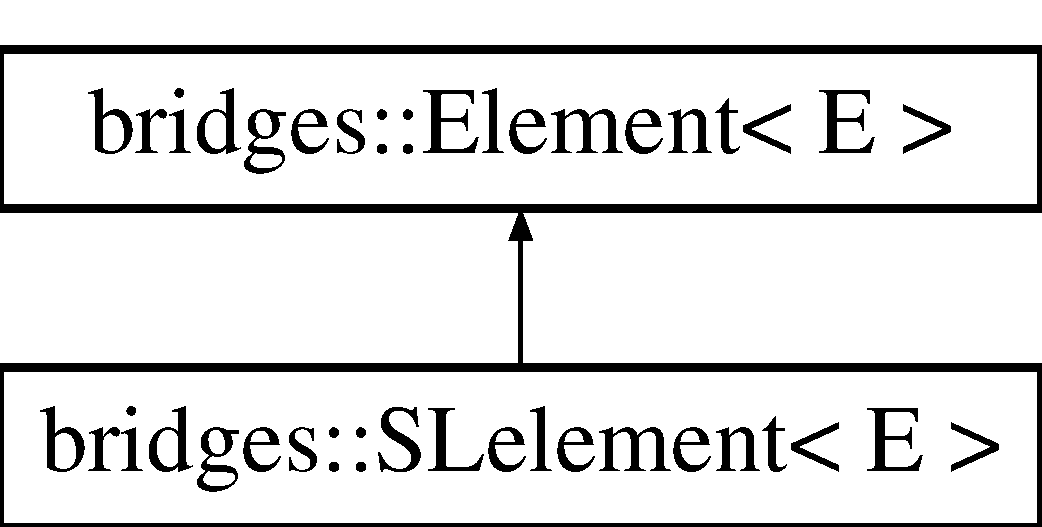
\includegraphics[height=2.000000cm]{classbridges_1_1_s_lelement}
\end{center}
\end{figure}
\subsection*{Public Member Functions}
\begin{DoxyCompactItemize}
\item 
\hyperlink{classbridges_1_1_s_lelement_a3e6d801b38ff3b1c4d2f5af50c070064}{S\+Lelement} ()
\item 
\hyperlink{classbridges_1_1_s_lelement_a04f5aac53435b59ee78dedccd5ceb2c9}{S\+Lelement} (string label, E e)
\item 
\hyperlink{classbridges_1_1_s_lelement_a3b6c621cbe6d1f7226e445f0c27b29f4}{S\+Lelement} (E e, \hyperlink{classbridges_1_1_s_lelement}{S\+Lelement}$<$ E $>$ $\ast$next)
\item 
\hyperlink{classbridges_1_1_s_lelement_a1b5ef640621cc8071194b5ccd976e2eb}{S\+Lelement} (\hyperlink{classbridges_1_1_s_lelement}{S\+Lelement}$<$ E $>$ $\ast$next)
\item 
\hyperlink{classbridges_1_1_s_lelement}{S\+Lelement}$<$ E $>$ $\ast$ \hyperlink{classbridges_1_1_s_lelement_aa11794bee00e3573c2e28786d57697dc}{get\+Next} ()
\item 
void \hyperlink{classbridges_1_1_s_lelement_a1faf256441dc4c4b4776ae3530d24a28}{set\+Next} (\hyperlink{classbridges_1_1_s_lelement}{S\+Lelement}$<$ E $>$ $\ast$next)
\end{DoxyCompactItemize}


\subsection{Constructor \& Destructor Documentation}
\hypertarget{classbridges_1_1_s_lelement_a3e6d801b38ff3b1c4d2f5af50c070064}{}\index{bridges\+::\+S\+Lelement@{bridges\+::\+S\+Lelement}!S\+Lelement@{S\+Lelement}}
\index{S\+Lelement@{S\+Lelement}!bridges\+::\+S\+Lelement@{bridges\+::\+S\+Lelement}}
\subsubsection[{S\+Lelement}]{\setlength{\rightskip}{0pt plus 5cm}template$<$typename E$>$ {\bf bridges\+::\+S\+Lelement}$<$ E $>$\+::{\bf S\+Lelement} (
\begin{DoxyParamCaption}
{}
\end{DoxyParamCaption}
)\hspace{0.3cm}{\ttfamily [inline]}}\label{classbridges_1_1_s_lelement_a3e6d801b38ff3b1c4d2f5af50c070064}
This constructor creates an \hyperlink{classbridges_1_1_s_lelement}{S\+Lelement} object with no parameters Both label and the application data need to be set separately. \hypertarget{classbridges_1_1_s_lelement_a04f5aac53435b59ee78dedccd5ceb2c9}{}\index{bridges\+::\+S\+Lelement@{bridges\+::\+S\+Lelement}!S\+Lelement@{S\+Lelement}}
\index{S\+Lelement@{S\+Lelement}!bridges\+::\+S\+Lelement@{bridges\+::\+S\+Lelement}}
\subsubsection[{S\+Lelement}]{\setlength{\rightskip}{0pt plus 5cm}template$<$typename E$>$ {\bf bridges\+::\+S\+Lelement}$<$ E $>$\+::{\bf S\+Lelement} (
\begin{DoxyParamCaption}
\item[{string}]{label, }
\item[{E}]{e}
\end{DoxyParamCaption}
)\hspace{0.3cm}{\ttfamily [inline]}}\label{classbridges_1_1_s_lelement_a04f5aac53435b59ee78dedccd5ceb2c9}
This constructor creates an \hyperlink{classbridges_1_1_s_lelement}{S\+Lelement} object of value \char`\"{}e\char`\"{} and label \char`\"{}label\char`\"{} and sets the next pointer to null 
\begin{DoxyParams}{Parameters}
{\em label} & the label of \hyperlink{classbridges_1_1_s_lelement}{S\+Lelement} that shows up on the \hyperlink{classbridges_1_1_bridges}{Bridges} visualization \\
\hline
{\em e} & the generic object that this \hyperlink{classbridges_1_1_s_lelement}{S\+Lelement} will hold \\
\hline
\end{DoxyParams}
\hypertarget{classbridges_1_1_s_lelement_a3b6c621cbe6d1f7226e445f0c27b29f4}{}\index{bridges\+::\+S\+Lelement@{bridges\+::\+S\+Lelement}!S\+Lelement@{S\+Lelement}}
\index{S\+Lelement@{S\+Lelement}!bridges\+::\+S\+Lelement@{bridges\+::\+S\+Lelement}}
\subsubsection[{S\+Lelement}]{\setlength{\rightskip}{0pt plus 5cm}template$<$typename E$>$ {\bf bridges\+::\+S\+Lelement}$<$ E $>$\+::{\bf S\+Lelement} (
\begin{DoxyParamCaption}
\item[{E}]{e, }
\item[{{\bf S\+Lelement}$<$ E $>$ $\ast$}]{next}
\end{DoxyParamCaption}
)\hspace{0.3cm}{\ttfamily [inline]}}\label{classbridges_1_1_s_lelement_a3b6c621cbe6d1f7226e445f0c27b29f4}
Creates a new element with value \char`\"{}e\char`\"{} and sets the next pointer to the \hyperlink{classbridges_1_1_s_lelement}{S\+Lelement} referenced by the \char`\"{}next\char`\"{} argument 
\begin{DoxyParams}{Parameters}
{\em e} & the generic object that this \hyperlink{classbridges_1_1_s_lelement}{S\+Lelement} will hold \\
\hline
{\em next} & the \hyperlink{classbridges_1_1_s_lelement}{S\+Lelement} that should be assigned to the next pointer \\
\hline
\end{DoxyParams}
\hypertarget{classbridges_1_1_s_lelement_a1b5ef640621cc8071194b5ccd976e2eb}{}\index{bridges\+::\+S\+Lelement@{bridges\+::\+S\+Lelement}!S\+Lelement@{S\+Lelement}}
\index{S\+Lelement@{S\+Lelement}!bridges\+::\+S\+Lelement@{bridges\+::\+S\+Lelement}}
\subsubsection[{S\+Lelement}]{\setlength{\rightskip}{0pt plus 5cm}template$<$typename E$>$ {\bf bridges\+::\+S\+Lelement}$<$ E $>$\+::{\bf S\+Lelement} (
\begin{DoxyParamCaption}
\item[{{\bf S\+Lelement}$<$ E $>$ $\ast$}]{next}
\end{DoxyParamCaption}
)\hspace{0.3cm}{\ttfamily [inline]}}\label{classbridges_1_1_s_lelement_a1b5ef640621cc8071194b5ccd976e2eb}
Creates a new element and sets the next pointer to the \hyperlink{classbridges_1_1_s_lelement}{S\+Lelement} \char`\"{}next\char`\"{} 
\begin{DoxyParams}{Parameters}
{\em next} & the \hyperlink{classbridges_1_1_s_lelement}{S\+Lelement} that should be assigned to the next pointer \\
\hline
\end{DoxyParams}


\subsection{Member Function Documentation}
\hypertarget{classbridges_1_1_s_lelement_aa11794bee00e3573c2e28786d57697dc}{}\index{bridges\+::\+S\+Lelement@{bridges\+::\+S\+Lelement}!get\+Next@{get\+Next}}
\index{get\+Next@{get\+Next}!bridges\+::\+S\+Lelement@{bridges\+::\+S\+Lelement}}
\subsubsection[{get\+Next}]{\setlength{\rightskip}{0pt plus 5cm}template$<$typename E$>$ {\bf S\+Lelement}$<$E$>$$\ast$ {\bf bridges\+::\+S\+Lelement}$<$ E $>$\+::get\+Next (
\begin{DoxyParamCaption}
{}
\end{DoxyParamCaption}
)\hspace{0.3cm}{\ttfamily [inline]}}\label{classbridges_1_1_s_lelement_aa11794bee00e3573c2e28786d57697dc}
Retrieves the next \hyperlink{classbridges_1_1_s_lelement}{S\+Lelement} \begin{DoxyReturn}{Returns}
S\+Lelement$<$\+E$>$ assigned to next 
\end{DoxyReturn}
\hypertarget{classbridges_1_1_s_lelement_a1faf256441dc4c4b4776ae3530d24a28}{}\index{bridges\+::\+S\+Lelement@{bridges\+::\+S\+Lelement}!set\+Next@{set\+Next}}
\index{set\+Next@{set\+Next}!bridges\+::\+S\+Lelement@{bridges\+::\+S\+Lelement}}
\subsubsection[{set\+Next}]{\setlength{\rightskip}{0pt plus 5cm}template$<$typename E$>$ void {\bf bridges\+::\+S\+Lelement}$<$ E $>$\+::set\+Next (
\begin{DoxyParamCaption}
\item[{{\bf S\+Lelement}$<$ E $>$ $\ast$}]{next}
\end{DoxyParamCaption}
)\hspace{0.3cm}{\ttfamily [inline]}}\label{classbridges_1_1_s_lelement_a1faf256441dc4c4b4776ae3530d24a28}
Sets the pointer to the next \hyperlink{classbridges_1_1_s_lelement}{S\+Lelement} 
\begin{DoxyParams}{Parameters}
{\em next} & S\+Lelement$<$\+E$>$ that should be assigned to the next pointer \\
\hline
\end{DoxyParams}


The documentation for this class was generated from the following file\+:\begin{DoxyCompactItemize}
\item 
src/\hyperlink{_s_lelement_8h}{S\+Lelement.\+h}\end{DoxyCompactItemize}

\hypertarget{classbridges_1_1_tree_element}{}\section{bridges\+:\+:Tree\+Element$<$ E $>$ Class Template Reference}
\label{classbridges_1_1_tree_element}\index{bridges\+::\+Tree\+Element$<$ E $>$@{bridges\+::\+Tree\+Element$<$ E $>$}}


{\ttfamily \#include $<$Tree\+Element.\+h$>$}

Inheritance diagram for bridges\+:\+:Tree\+Element$<$ E $>$\+:\begin{figure}[H]
\begin{center}
\leavevmode
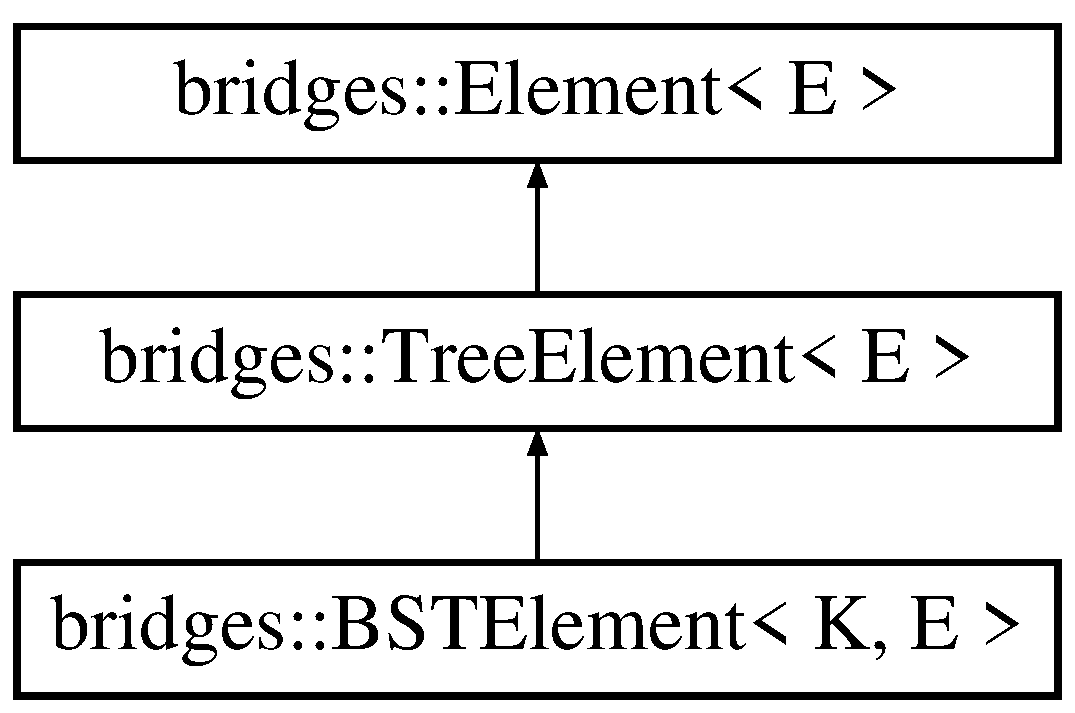
\includegraphics[height=3.000000cm]{classbridges_1_1_tree_element}
\end{center}
\end{figure}
\subsection*{Public Member Functions}
\begin{DoxyCompactItemize}
\item 
\hyperlink{classbridges_1_1_tree_element_a75e7d67cc9357820e9e5ce6ab0370be8}{Tree\+Element} ()
\item 
\hyperlink{classbridges_1_1_tree_element_a03a6eb569c829d3a70364f93e5241d72}{Tree\+Element} (const \hyperlink{classbridges_1_1_tree_element}{Tree\+Element}$<$ E $>$ \&te)
\item 
\hyperlink{classbridges_1_1_tree_element_ab0f11470f6983709436c700956398d78}{Tree\+Element} (E e)
\item 
\hyperlink{classbridges_1_1_tree_element_a6b5c2150ee4297fb7b341eb7d373492e}{Tree\+Element} (string label, E e)
\item 
\hyperlink{classbridges_1_1_tree_element_aa7af1081512887f5ce22ab47fe8f8624}{Tree\+Element} (\hyperlink{classbridges_1_1_tree_element}{Tree\+Element}$<$ E $>$ $\ast$left, \hyperlink{classbridges_1_1_tree_element}{Tree\+Element}$<$ E $>$ $\ast$right)
\item 
\hyperlink{classbridges_1_1_tree_element_a23151bf7f36d7f3f9e311a032d932c88}{Tree\+Element} (E e, \hyperlink{classbridges_1_1_tree_element}{Tree\+Element}$<$ E $>$ $\ast$left, \hyperlink{classbridges_1_1_tree_element}{Tree\+Element}$<$ E $>$ $\ast$right)
\item 
\hyperlink{classbridges_1_1_tree_element}{Tree\+Element}$<$ E $>$ $\ast$ \hyperlink{classbridges_1_1_tree_element_ad40ac069fa73faa46ff0398af1045c66}{get\+Left} ()
\item 
void \hyperlink{classbridges_1_1_tree_element_a68ab81b0b7da1c81f3bfbabe918a0d1a}{set\+Left} (\hyperlink{classbridges_1_1_tree_element}{Tree\+Element}$<$ E $>$ $\ast$left)
\item 
\hyperlink{classbridges_1_1_tree_element}{Tree\+Element}$<$ E $>$ $\ast$ \hyperlink{classbridges_1_1_tree_element_ae6e7ea308f95522c79ea5ca84bdbe2c1}{get\+Right} ()
\item 
void \hyperlink{classbridges_1_1_tree_element_a6c4018bbbc0597278bccf3809ed4485f}{set\+Right} (\hyperlink{classbridges_1_1_tree_element}{Tree\+Element}$<$ E $>$ $\ast$right)
\end{DoxyCompactItemize}


\subsection{Constructor \& Destructor Documentation}
\hypertarget{classbridges_1_1_tree_element_a75e7d67cc9357820e9e5ce6ab0370be8}{}\index{bridges\+::\+Tree\+Element@{bridges\+::\+Tree\+Element}!Tree\+Element@{Tree\+Element}}
\index{Tree\+Element@{Tree\+Element}!bridges\+::\+Tree\+Element@{bridges\+::\+Tree\+Element}}
\subsubsection[{Tree\+Element}]{\setlength{\rightskip}{0pt plus 5cm}template$<$typename E$>$ {\bf bridges\+::\+Tree\+Element}$<$ E $>$\+::{\bf Tree\+Element} (
\begin{DoxyParamCaption}
{}
\end{DoxyParamCaption}
)\hspace{0.3cm}{\ttfamily [inline]}}\label{classbridges_1_1_tree_element_a75e7d67cc9357820e9e5ce6ab0370be8}
Constructs an empty \hyperlink{classbridges_1_1_tree_element}{Tree\+Element} with right and left pointers set to null. \hypertarget{classbridges_1_1_tree_element_a03a6eb569c829d3a70364f93e5241d72}{}\index{bridges\+::\+Tree\+Element@{bridges\+::\+Tree\+Element}!Tree\+Element@{Tree\+Element}}
\index{Tree\+Element@{Tree\+Element}!bridges\+::\+Tree\+Element@{bridges\+::\+Tree\+Element}}
\subsubsection[{Tree\+Element}]{\setlength{\rightskip}{0pt plus 5cm}template$<$typename E$>$ {\bf bridges\+::\+Tree\+Element}$<$ E $>$\+::{\bf Tree\+Element} (
\begin{DoxyParamCaption}
\item[{const {\bf Tree\+Element}$<$ E $>$ \&}]{te}
\end{DoxyParamCaption}
)\hspace{0.3cm}{\ttfamily [inline]}}\label{classbridges_1_1_tree_element_a03a6eb569c829d3a70364f93e5241d72}
\hypertarget{classbridges_1_1_tree_element_ab0f11470f6983709436c700956398d78}{}\index{bridges\+::\+Tree\+Element@{bridges\+::\+Tree\+Element}!Tree\+Element@{Tree\+Element}}
\index{Tree\+Element@{Tree\+Element}!bridges\+::\+Tree\+Element@{bridges\+::\+Tree\+Element}}
\subsubsection[{Tree\+Element}]{\setlength{\rightskip}{0pt plus 5cm}template$<$typename E$>$ {\bf bridges\+::\+Tree\+Element}$<$ E $>$\+::{\bf Tree\+Element} (
\begin{DoxyParamCaption}
\item[{E}]{e}
\end{DoxyParamCaption}
)\hspace{0.3cm}{\ttfamily [inline]}}\label{classbridges_1_1_tree_element_ab0f11470f6983709436c700956398d78}
Constructs a \hyperlink{classbridges_1_1_tree_element}{Tree\+Element} holding an object \char`\"{}e\char`\"{} with right and left pointers set to null. 
\begin{DoxyParams}{Parameters}
{\em e} & the generic object that \hyperlink{classbridges_1_1_tree_element}{Tree\+Element} will hold \\
\hline
\end{DoxyParams}
\hypertarget{classbridges_1_1_tree_element_a6b5c2150ee4297fb7b341eb7d373492e}{}\index{bridges\+::\+Tree\+Element@{bridges\+::\+Tree\+Element}!Tree\+Element@{Tree\+Element}}
\index{Tree\+Element@{Tree\+Element}!bridges\+::\+Tree\+Element@{bridges\+::\+Tree\+Element}}
\subsubsection[{Tree\+Element}]{\setlength{\rightskip}{0pt plus 5cm}template$<$typename E$>$ {\bf bridges\+::\+Tree\+Element}$<$ E $>$\+::{\bf Tree\+Element} (
\begin{DoxyParamCaption}
\item[{string}]{label, }
\item[{E}]{e}
\end{DoxyParamCaption}
)\hspace{0.3cm}{\ttfamily [inline]}}\label{classbridges_1_1_tree_element_a6b5c2150ee4297fb7b341eb7d373492e}
Constructs a \hyperlink{classbridges_1_1_tree_element}{Tree\+Element} with label set to \char`\"{}label\char`\"{}, holding an object \char`\"{}e\char`\"{}. 
\begin{DoxyParams}{Parameters}
{\em label} & the label of \hyperlink{classbridges_1_1_tree_element}{Tree\+Element} that shows up on the \hyperlink{classbridges_1_1_bridges}{Bridges} visualization \\
\hline
{\em e} & the generic object that \hyperlink{classbridges_1_1_tree_element}{Tree\+Element} will hold \\
\hline
\end{DoxyParams}
\hypertarget{classbridges_1_1_tree_element_aa7af1081512887f5ce22ab47fe8f8624}{}\index{bridges\+::\+Tree\+Element@{bridges\+::\+Tree\+Element}!Tree\+Element@{Tree\+Element}}
\index{Tree\+Element@{Tree\+Element}!bridges\+::\+Tree\+Element@{bridges\+::\+Tree\+Element}}
\subsubsection[{Tree\+Element}]{\setlength{\rightskip}{0pt plus 5cm}template$<$typename E$>$ {\bf bridges\+::\+Tree\+Element}$<$ E $>$\+::{\bf Tree\+Element} (
\begin{DoxyParamCaption}
\item[{{\bf Tree\+Element}$<$ E $>$ $\ast$}]{left, }
\item[{{\bf Tree\+Element}$<$ E $>$ $\ast$}]{right}
\end{DoxyParamCaption}
)\hspace{0.3cm}{\ttfamily [inline]}}\label{classbridges_1_1_tree_element_aa7af1081512887f5ce22ab47fe8f8624}
Construct a \hyperlink{classbridges_1_1_tree_element}{Tree\+Element} with 
\begin{DoxyParams}{Parameters}
{\em left} & the \hyperlink{classbridges_1_1_tree_element}{Tree\+Element} to be assigned to the left pointer of this \hyperlink{classbridges_1_1_tree_element}{Tree\+Element} \\
\hline
{\em right} & the \hyperlink{classbridges_1_1_tree_element}{Tree\+Element} to be assigned to the right pointer of this \hyperlink{classbridges_1_1_tree_element}{Tree\+Element} \\
\hline
\end{DoxyParams}
\hypertarget{classbridges_1_1_tree_element_a23151bf7f36d7f3f9e311a032d932c88}{}\index{bridges\+::\+Tree\+Element@{bridges\+::\+Tree\+Element}!Tree\+Element@{Tree\+Element}}
\index{Tree\+Element@{Tree\+Element}!bridges\+::\+Tree\+Element@{bridges\+::\+Tree\+Element}}
\subsubsection[{Tree\+Element}]{\setlength{\rightskip}{0pt plus 5cm}template$<$typename E$>$ {\bf bridges\+::\+Tree\+Element}$<$ E $>$\+::{\bf Tree\+Element} (
\begin{DoxyParamCaption}
\item[{E}]{e, }
\item[{{\bf Tree\+Element}$<$ E $>$ $\ast$}]{left, }
\item[{{\bf Tree\+Element}$<$ E $>$ $\ast$}]{right}
\end{DoxyParamCaption}
)\hspace{0.3cm}{\ttfamily [inline]}}\label{classbridges_1_1_tree_element_a23151bf7f36d7f3f9e311a032d932c88}
Constructs a \hyperlink{classbridges_1_1_tree_element}{Tree\+Element} holding the object \char`\"{}e\char`\"{}, left pointer pointing to \char`\"{}left\char`\"{} and right pointer pointing to \char`\"{}right\char`\"{}. 
\begin{DoxyParams}{Parameters}
{\em e} & the generic object that \hyperlink{classbridges_1_1_tree_element}{Tree\+Element} will hold \\
\hline
{\em left} & the \hyperlink{classbridges_1_1_tree_element}{Tree\+Element} to be assigned to the left pointer of this \hyperlink{classbridges_1_1_tree_element}{Tree\+Element} \\
\hline
{\em right} & the \hyperlink{classbridges_1_1_tree_element}{Tree\+Element} to be assigned to the right pointer of this \hyperlink{classbridges_1_1_tree_element}{Tree\+Element} \\
\hline
\end{DoxyParams}


\subsection{Member Function Documentation}
\hypertarget{classbridges_1_1_tree_element_ad40ac069fa73faa46ff0398af1045c66}{}\index{bridges\+::\+Tree\+Element@{bridges\+::\+Tree\+Element}!get\+Left@{get\+Left}}
\index{get\+Left@{get\+Left}!bridges\+::\+Tree\+Element@{bridges\+::\+Tree\+Element}}
\subsubsection[{get\+Left}]{\setlength{\rightskip}{0pt plus 5cm}template$<$typename E$>$ {\bf Tree\+Element}$<$E$>$$\ast$ {\bf bridges\+::\+Tree\+Element}$<$ E $>$\+::get\+Left (
\begin{DoxyParamCaption}
{}
\end{DoxyParamCaption}
)\hspace{0.3cm}{\ttfamily [inline]}}\label{classbridges_1_1_tree_element_ad40ac069fa73faa46ff0398af1045c66}
This method returns the left tree element pointer \begin{DoxyReturn}{Returns}
the left child of this \hyperlink{classbridges_1_1_tree_element}{Tree\+Element} 
\end{DoxyReturn}
\hypertarget{classbridges_1_1_tree_element_ae6e7ea308f95522c79ea5ca84bdbe2c1}{}\index{bridges\+::\+Tree\+Element@{bridges\+::\+Tree\+Element}!get\+Right@{get\+Right}}
\index{get\+Right@{get\+Right}!bridges\+::\+Tree\+Element@{bridges\+::\+Tree\+Element}}
\subsubsection[{get\+Right}]{\setlength{\rightskip}{0pt plus 5cm}template$<$typename E$>$ {\bf Tree\+Element}$<$E$>$$\ast$ {\bf bridges\+::\+Tree\+Element}$<$ E $>$\+::get\+Right (
\begin{DoxyParamCaption}
{}
\end{DoxyParamCaption}
)\hspace{0.3cm}{\ttfamily [inline]}}\label{classbridges_1_1_tree_element_ae6e7ea308f95522c79ea5ca84bdbe2c1}
This method returns the right tree element pointer \begin{DoxyReturn}{Returns}
the right child of this \hyperlink{classbridges_1_1_tree_element}{Tree\+Element} 
\end{DoxyReturn}
\hypertarget{classbridges_1_1_tree_element_a68ab81b0b7da1c81f3bfbabe918a0d1a}{}\index{bridges\+::\+Tree\+Element@{bridges\+::\+Tree\+Element}!set\+Left@{set\+Left}}
\index{set\+Left@{set\+Left}!bridges\+::\+Tree\+Element@{bridges\+::\+Tree\+Element}}
\subsubsection[{set\+Left}]{\setlength{\rightskip}{0pt plus 5cm}template$<$typename E$>$ void {\bf bridges\+::\+Tree\+Element}$<$ E $>$\+::set\+Left (
\begin{DoxyParamCaption}
\item[{{\bf Tree\+Element}$<$ E $>$ $\ast$}]{left}
\end{DoxyParamCaption}
)\hspace{0.3cm}{\ttfamily [inline]}}\label{classbridges_1_1_tree_element_a68ab81b0b7da1c81f3bfbabe918a0d1a}
This method sets the left tree element pointer 
\begin{DoxyParams}{Parameters}
{\em left} & the \hyperlink{classbridges_1_1_tree_element}{Tree\+Element} that should be assigned to the left child \\
\hline
\end{DoxyParams}
\hypertarget{classbridges_1_1_tree_element_a6c4018bbbc0597278bccf3809ed4485f}{}\index{bridges\+::\+Tree\+Element@{bridges\+::\+Tree\+Element}!set\+Right@{set\+Right}}
\index{set\+Right@{set\+Right}!bridges\+::\+Tree\+Element@{bridges\+::\+Tree\+Element}}
\subsubsection[{set\+Right}]{\setlength{\rightskip}{0pt plus 5cm}template$<$typename E$>$ void {\bf bridges\+::\+Tree\+Element}$<$ E $>$\+::set\+Right (
\begin{DoxyParamCaption}
\item[{{\bf Tree\+Element}$<$ E $>$ $\ast$}]{right}
\end{DoxyParamCaption}
)\hspace{0.3cm}{\ttfamily [inline]}}\label{classbridges_1_1_tree_element_a6c4018bbbc0597278bccf3809ed4485f}
This method sets the right tree element pointer 
\begin{DoxyParams}{Parameters}
{\em right} & the \hyperlink{classbridges_1_1_tree_element}{Tree\+Element} that should be assigned to the right child \\
\hline
\end{DoxyParams}


The documentation for this class was generated from the following file\+:\begin{DoxyCompactItemize}
\item 
src/\hyperlink{_tree_element_8h}{Tree\+Element.\+h}\end{DoxyCompactItemize}

\hypertarget{classbridges_1_1_validation}{}\section{bridges\+:\+:Validation Class Reference}
\label{classbridges_1_1_validation}\index{bridges\+::\+Validation@{bridges\+::\+Validation}}


{\ttfamily \#include $<$Validation.\+h$>$}

\subsection*{Public Member Functions}
\begin{DoxyCompactItemize}
\item 
\hyperlink{classbridges_1_1_validation_af96b099ca6ce6cd4f408f1cead574d72}{Validation} ()
\item 
void \hyperlink{classbridges_1_1_validation_ae996957e1fc7f77ef49c31fbdb787933}{validate\+Color} (string color)
\item 
void \hyperlink{classbridges_1_1_validation_aeb22afdeb015c9d9015889a240918542}{validate\+Shape} (string shape)
\item 
void \hyperlink{classbridges_1_1_validation_a1e3a732becc5d60df177ac2db2795885}{validate\+Opacity} (double val)
\item 
void \hyperlink{classbridges_1_1_validation_a323312df77e8efe8382a25ff7295819d}{validate\+Size} (double val)
\item 
void \hyperlink{classbridges_1_1_validation_a234922474be2e46f8b34d50c618716a3}{validate\+Thickness} (double val)
\item 
void \hyperlink{classbridges_1_1_validation_a75e8636360983f0b12fb7e6581a02357}{validate\+Weight} (int val)
\item 
void \hyperlink{classbridges_1_1_validation_a79c78d43b8226b0b53da078458941117}{validate\+\_\+\+A\+D\+T\+\_\+size} (int max\+\_\+elements)
\end{DoxyCompactItemize}
\subsection*{Static Public Member Functions}
\begin{DoxyCompactItemize}
\item 
static \hyperlink{classbridges_1_1_validation}{Validation} $\ast$ \hyperlink{classbridges_1_1_validation_add1944b1167e0e6b1a80e303b3a16b5b}{get\+Current} ()
\end{DoxyCompactItemize}


\subsection{Constructor \& Destructor Documentation}
\hypertarget{classbridges_1_1_validation_af96b099ca6ce6cd4f408f1cead574d72}{}\index{bridges\+::\+Validation@{bridges\+::\+Validation}!Validation@{Validation}}
\index{Validation@{Validation}!bridges\+::\+Validation@{bridges\+::\+Validation}}
\subsubsection[{Validation}]{\setlength{\rightskip}{0pt plus 5cm}bridges\+::\+Validation\+::\+Validation (
\begin{DoxyParamCaption}
{}
\end{DoxyParamCaption}
)\hspace{0.3cm}{\ttfamily [inline]}}\label{classbridges_1_1_validation_af96b099ca6ce6cd4f408f1cead574d72}


\subsection{Member Function Documentation}
\hypertarget{classbridges_1_1_validation_add1944b1167e0e6b1a80e303b3a16b5b}{}\index{bridges\+::\+Validation@{bridges\+::\+Validation}!get\+Current@{get\+Current}}
\index{get\+Current@{get\+Current}!bridges\+::\+Validation@{bridges\+::\+Validation}}
\subsubsection[{get\+Current}]{\setlength{\rightskip}{0pt plus 5cm}static {\bf Validation}$\ast$ bridges\+::\+Validation\+::get\+Current (
\begin{DoxyParamCaption}
{}
\end{DoxyParamCaption}
)\hspace{0.3cm}{\ttfamily [inline]}, {\ttfamily [static]}}\label{classbridges_1_1_validation_add1944b1167e0e6b1a80e303b3a16b5b}
Gets the current \hyperlink{classbridges_1_1_validation}{Validation} object -\/ used in various other \hyperlink{classbridges_1_1_bridges}{Bridges} classes to do validation of visual properties input by the user \hypertarget{classbridges_1_1_validation_a79c78d43b8226b0b53da078458941117}{}\index{bridges\+::\+Validation@{bridges\+::\+Validation}!validate\+\_\+\+A\+D\+T\+\_\+size@{validate\+\_\+\+A\+D\+T\+\_\+size}}
\index{validate\+\_\+\+A\+D\+T\+\_\+size@{validate\+\_\+\+A\+D\+T\+\_\+size}!bridges\+::\+Validation@{bridges\+::\+Validation}}
\subsubsection[{validate\+\_\+\+A\+D\+T\+\_\+size}]{\setlength{\rightskip}{0pt plus 5cm}void bridges\+::\+Validation\+::validate\+\_\+\+A\+D\+T\+\_\+size (
\begin{DoxyParamCaption}
\item[{int}]{max\+\_\+elements}
\end{DoxyParamCaption}
)\hspace{0.3cm}{\ttfamily [inline]}}\label{classbridges_1_1_validation_a79c78d43b8226b0b53da078458941117}
\hypertarget{classbridges_1_1_validation_ae996957e1fc7f77ef49c31fbdb787933}{}\index{bridges\+::\+Validation@{bridges\+::\+Validation}!validate\+Color@{validate\+Color}}
\index{validate\+Color@{validate\+Color}!bridges\+::\+Validation@{bridges\+::\+Validation}}
\subsubsection[{validate\+Color}]{\setlength{\rightskip}{0pt plus 5cm}void bridges\+::\+Validation\+::validate\+Color (
\begin{DoxyParamCaption}
\item[{string}]{color}
\end{DoxyParamCaption}
)\hspace{0.3cm}{\ttfamily [inline]}}\label{classbridges_1_1_validation_ae996957e1fc7f77ef49c31fbdb787933}
Determine if a color is supported by C\+S\+S.

This method only supports a subject of C\+S\+S (yet). (1) 173 C\+S\+S extended color names, (2) \#\+R\+R\+G\+G\+B\+B or \#\+R\+G\+B, where R, G and B are red, green, blue values as hexadecimal digits.

This method does not check for null because null has special meaning.


\begin{DoxyParams}{Parameters}
{\em color} & \\
\hline
\end{DoxyParams}
\begin{DoxyReturn}{Returns}
whether the color is valid 
\end{DoxyReturn}
\hypertarget{classbridges_1_1_validation_a1e3a732becc5d60df177ac2db2795885}{}\index{bridges\+::\+Validation@{bridges\+::\+Validation}!validate\+Opacity@{validate\+Opacity}}
\index{validate\+Opacity@{validate\+Opacity}!bridges\+::\+Validation@{bridges\+::\+Validation}}
\subsubsection[{validate\+Opacity}]{\setlength{\rightskip}{0pt plus 5cm}void bridges\+::\+Validation\+::validate\+Opacity (
\begin{DoxyParamCaption}
\item[{double}]{val}
\end{DoxyParamCaption}
)\hspace{0.3cm}{\ttfamily [inline]}}\label{classbridges_1_1_validation_a1e3a732becc5d60df177ac2db2795885}
Determines if the value passed is an acceptable value to set the opacity to.


\begin{DoxyParams}{Parameters}
{\em val} & \\
\hline
\end{DoxyParams}
\hypertarget{classbridges_1_1_validation_aeb22afdeb015c9d9015889a240918542}{}\index{bridges\+::\+Validation@{bridges\+::\+Validation}!validate\+Shape@{validate\+Shape}}
\index{validate\+Shape@{validate\+Shape}!bridges\+::\+Validation@{bridges\+::\+Validation}}
\subsubsection[{validate\+Shape}]{\setlength{\rightskip}{0pt plus 5cm}void bridges\+::\+Validation\+::validate\+Shape (
\begin{DoxyParamCaption}
\item[{string}]{shape}
\end{DoxyParamCaption}
)\hspace{0.3cm}{\ttfamily [inline]}}\label{classbridges_1_1_validation_aeb22afdeb015c9d9015889a240918542}
Determines if the shape is supported.


\begin{DoxyParams}{Parameters}
{\em shape} & \\
\hline
\end{DoxyParams}
\hypertarget{classbridges_1_1_validation_a323312df77e8efe8382a25ff7295819d}{}\index{bridges\+::\+Validation@{bridges\+::\+Validation}!validate\+Size@{validate\+Size}}
\index{validate\+Size@{validate\+Size}!bridges\+::\+Validation@{bridges\+::\+Validation}}
\subsubsection[{validate\+Size}]{\setlength{\rightskip}{0pt plus 5cm}void bridges\+::\+Validation\+::validate\+Size (
\begin{DoxyParamCaption}
\item[{double}]{val}
\end{DoxyParamCaption}
)\hspace{0.3cm}{\ttfamily [inline]}}\label{classbridges_1_1_validation_a323312df77e8efe8382a25ff7295819d}
Determines if the value passed is an acceptable value to set the size to.


\begin{DoxyParams}{Parameters}
{\em val} & \\
\hline
\end{DoxyParams}
\hypertarget{classbridges_1_1_validation_a234922474be2e46f8b34d50c618716a3}{}\index{bridges\+::\+Validation@{bridges\+::\+Validation}!validate\+Thickness@{validate\+Thickness}}
\index{validate\+Thickness@{validate\+Thickness}!bridges\+::\+Validation@{bridges\+::\+Validation}}
\subsubsection[{validate\+Thickness}]{\setlength{\rightskip}{0pt plus 5cm}void bridges\+::\+Validation\+::validate\+Thickness (
\begin{DoxyParamCaption}
\item[{double}]{val}
\end{DoxyParamCaption}
)\hspace{0.3cm}{\ttfamily [inline]}}\label{classbridges_1_1_validation_a234922474be2e46f8b34d50c618716a3}
Determines if the value passed is an acceptable value to set the thickness to.


\begin{DoxyParams}{Parameters}
{\em val} & \\
\hline
\end{DoxyParams}
\hypertarget{classbridges_1_1_validation_a75e8636360983f0b12fb7e6581a02357}{}\index{bridges\+::\+Validation@{bridges\+::\+Validation}!validate\+Weight@{validate\+Weight}}
\index{validate\+Weight@{validate\+Weight}!bridges\+::\+Validation@{bridges\+::\+Validation}}
\subsubsection[{validate\+Weight}]{\setlength{\rightskip}{0pt plus 5cm}void bridges\+::\+Validation\+::validate\+Weight (
\begin{DoxyParamCaption}
\item[{int}]{val}
\end{DoxyParamCaption}
)\hspace{0.3cm}{\ttfamily [inline]}}\label{classbridges_1_1_validation_a75e8636360983f0b12fb7e6581a02357}
Determines if the value passed is an acceptable value to set the weight to -\/ must be positive.


\begin{DoxyParams}{Parameters}
{\em val} & \\
\hline
\end{DoxyParams}


The documentation for this class was generated from the following file\+:\begin{DoxyCompactItemize}
\item 
src/\hyperlink{_validation_8h}{Validation.\+h}\end{DoxyCompactItemize}

\chapter{File Documentation}
\hypertarget{_a_d_t_visualizer_8h}{}\section{src/\+A\+D\+T\+Visualizer.h File Reference}
\label{_a_d_t_visualizer_8h}\index{src/\+A\+D\+T\+Visualizer.\+h@{src/\+A\+D\+T\+Visualizer.\+h}}
{\ttfamily \#include $<$iostream$>$}\\*
{\ttfamily \#include $<$sstream$>$}\\*
{\ttfamily \#include $<$string$>$}\\*
{\ttfamily \#include $<$list$>$}\\*
{\ttfamily \#include $<$vector$>$}\\*
{\ttfamily \#include $<$unordered\+\_\+map$>$}\\*
{\ttfamily \#include \char`\"{}Graph\+Adj\+Matrix.\+h\char`\"{}}\\*
{\ttfamily \#include \char`\"{}Graph\+Adj\+List.\+h\char`\"{}}\\*
{\ttfamily \#include \char`\"{}D\+Lelement.\+h\char`\"{}}\\*
{\ttfamily \#include \char`\"{}Tree\+Element.\+h\char`\"{}}\\*
{\ttfamily \#include \char`\"{}B\+S\+T\+Element.\+h\char`\"{}}\\*
\subsection*{Classes}
\begin{DoxyCompactItemize}
\item 
class \hyperlink{classbridges_1_1_a_d_t_visualizer}{bridges\+::\+A\+D\+T\+Visualizer$<$ K, E $>$}
\end{DoxyCompactItemize}
\subsection*{Namespaces}
\begin{DoxyCompactItemize}
\item 
 \hyperlink{namespacebridges}{bridges}
\end{DoxyCompactItemize}

\hypertarget{_array_8h}{}\section{src/\+Array.h File Reference}
\label{_array_8h}\index{src/\+Array.\+h@{src/\+Array.\+h}}

\hypertarget{_bridges_8h}{}\section{src/\+Bridges.h File Reference}
\label{_bridges_8h}\index{src/\+Bridges.\+h@{src/\+Bridges.\+h}}
{\ttfamily \#include $<$iostream$>$}\\*
{\ttfamily \#include $<$string$>$}\\*
{\ttfamily \#include $<$unordered\+\_\+map$>$}\\*
{\ttfamily \#include $<$cmath$>$}\\*
{\ttfamily \#include $<$new$>$}\\*
{\ttfamily \#include \char`\"{}B\+S\+T\+Element.\+h\char`\"{}}\\*
{\ttfamily \#include \char`\"{}Connector.\+h\char`\"{}}\\*
{\ttfamily \#include \char`\"{}Graph\+Adj\+List.\+h\char`\"{}}\\*
{\ttfamily \#include \char`\"{}Graph\+Adj\+Matrix.\+h\char`\"{}}\\*
{\ttfamily \#include \char`\"{}Validation.\+h\char`\"{}}\\*
\subsection*{Classes}
\begin{DoxyCompactItemize}
\item 
class \hyperlink{classbridges_1_1_bridges}{bridges\+::\+Bridges$<$ K, E $>$}
\end{DoxyCompactItemize}
\subsection*{Namespaces}
\begin{DoxyCompactItemize}
\item 
 \hyperlink{namespacebridges}{bridges}
\end{DoxyCompactItemize}

\hypertarget{_b_s_t_element_8h}{}\section{src/\+B\+S\+T\+Element.h File Reference}
\label{_b_s_t_element_8h}\index{src/\+B\+S\+T\+Element.\+h@{src/\+B\+S\+T\+Element.\+h}}
{\ttfamily \#include $<$sstream$>$}\\*
{\ttfamily \#include $<$string$>$}\\*
{\ttfamily \#include \char`\"{}Tree\+Element.\+h\char`\"{}}\\*
\subsection*{Classes}
\begin{DoxyCompactItemize}
\item 
class \hyperlink{classbridges_1_1_b_s_t_element}{bridges\+::\+B\+S\+T\+Element$<$ K, E $>$}
\end{DoxyCompactItemize}
\subsection*{Namespaces}
\begin{DoxyCompactItemize}
\item 
 \hyperlink{namespacebridges}{bridges}
\end{DoxyCompactItemize}

\hypertarget{_connector_8h}{}\section{src/\+Connector.h File Reference}
\label{_connector_8h}\index{src/\+Connector.\+h@{src/\+Connector.\+h}}
{\ttfamily \#include $<$string$>$}\\*
{\ttfamily \#include $<$iostream$>$}\\*
{\ttfamily \#include $<$curl/curl.\+h$>$}\\*
{\ttfamily \#include \char`\"{}Element.\+h\char`\"{}}\\*
{\ttfamily \#include \char`\"{}A\+D\+T\+Visualizer.\+h\char`\"{}}\\*
\subsection*{Classes}
\begin{DoxyCompactItemize}
\item 
class \hyperlink{classbridges_1_1_connector}{bridges\+::\+Connector}
\end{DoxyCompactItemize}
\subsection*{Namespaces}
\begin{DoxyCompactItemize}
\item 
 \hyperlink{namespacebridges}{bridges}
\end{DoxyCompactItemize}

\hypertarget{_d_lelement_8h}{}\section{src/\+D\+Lelement.h File Reference}
\label{_d_lelement_8h}\index{src/\+D\+Lelement.\+h@{src/\+D\+Lelement.\+h}}
\subsection*{Classes}
\begin{DoxyCompactItemize}
\item 
class \hyperlink{classbridges_1_1_d_lelement}{bridges\+::\+D\+Lelement$<$ E $>$}
\end{DoxyCompactItemize}
\subsection*{Namespaces}
\begin{DoxyCompactItemize}
\item 
 \hyperlink{namespacebridges}{bridges}
\end{DoxyCompactItemize}

\hypertarget{_edge_8h}{}\section{src/\+Edge.h File Reference}
\label{_edge_8h}\index{src/\+Edge.\+h@{src/\+Edge.\+h}}
{\ttfamily \#include $<$string$>$}\\*
\subsection*{Classes}
\begin{DoxyCompactItemize}
\item 
class \hyperlink{classbridges_1_1_edge}{bridges\+::\+Edge$<$ Key $>$}
\end{DoxyCompactItemize}
\subsection*{Namespaces}
\begin{DoxyCompactItemize}
\item 
 \hyperlink{namespacebridges}{bridges}
\end{DoxyCompactItemize}

\hypertarget{_element_8h}{}\section{src/\+Element.h File Reference}
\label{_element_8h}\index{src/\+Element.\+h@{src/\+Element.\+h}}
{\ttfamily \#include $<$iostream$>$}\\*
{\ttfamily \#include $<$new$>$}\\*
{\ttfamily \#include $<$string$>$}\\*
{\ttfamily \#include $<$unordered\+\_\+map$>$}\\*
{\ttfamily \#include \char`\"{}Element\+Visualizer.\+h\char`\"{}}\\*
{\ttfamily \#include \char`\"{}Link\+Visualizer.\+h\char`\"{}}\\*
\subsection*{Classes}
\begin{DoxyCompactItemize}
\item 
class \hyperlink{classbridges_1_1_element}{bridges\+::\+Element$<$ E $>$}
\end{DoxyCompactItemize}
\subsection*{Namespaces}
\begin{DoxyCompactItemize}
\item 
 \hyperlink{namespacebridges}{bridges}
\end{DoxyCompactItemize}

\hypertarget{_element_visualizer_8h}{}\section{src/\+Element\+Visualizer.h File Reference}
\label{_element_visualizer_8h}\index{src/\+Element\+Visualizer.\+h@{src/\+Element\+Visualizer.\+h}}
{\ttfamily \#include $<$string$>$}\\*
{\ttfamily \#include $<$iostream$>$}\\*
{\ttfamily \#include $<$unordered\+\_\+map$>$}\\*
{\ttfamily \#include \char`\"{}Validation.\+h\char`\"{}}\\*
\subsection*{Classes}
\begin{DoxyCompactItemize}
\item 
class \hyperlink{classbridges_1_1_element_visualizer}{bridges\+::\+Element\+Visualizer}
\end{DoxyCompactItemize}
\subsection*{Namespaces}
\begin{DoxyCompactItemize}
\item 
 \hyperlink{namespacebridges}{bridges}
\end{DoxyCompactItemize}

\hypertarget{_graph_adj_list_8h}{}\section{src/\+Graph\+Adj\+List.h File Reference}
\label{_graph_adj_list_8h}\index{src/\+Graph\+Adj\+List.\+h@{src/\+Graph\+Adj\+List.\+h}}
{\ttfamily \#include $<$unordered\+\_\+map$>$}\\*
{\ttfamily \#include $<$sstream$>$}\\*
{\ttfamily \#include \char`\"{}S\+Lelement.\+h\char`\"{}}\\*
{\ttfamily \#include \char`\"{}Edge.\+h\char`\"{}}\\*
\subsection*{Classes}
\begin{DoxyCompactItemize}
\item 
class \hyperlink{classbridges_1_1_graph_adj_list}{bridges\+::\+Graph\+Adj\+List$<$ Key, E $>$}
\end{DoxyCompactItemize}
\subsection*{Namespaces}
\begin{DoxyCompactItemize}
\item 
 \hyperlink{namespacebridges}{bridges}
\end{DoxyCompactItemize}

\hypertarget{_graph_adj_matrix_8h}{}\section{src/\+Graph\+Adj\+Matrix.h File Reference}
\label{_graph_adj_matrix_8h}\index{src/\+Graph\+Adj\+Matrix.\+h@{src/\+Graph\+Adj\+Matrix.\+h}}
{\ttfamily \#include $<$string$>$}\\*
{\ttfamily \#include $<$sstream$>$}\\*
{\ttfamily \#include $<$unordered\+\_\+map$>$}\\*
\subsection*{Classes}
\begin{DoxyCompactItemize}
\item 
class \hyperlink{classbridges_1_1_graph_adj_matrix}{bridges\+::\+Graph\+Adj\+Matrix$<$ Key, E $>$}
\end{DoxyCompactItemize}
\subsection*{Namespaces}
\begin{DoxyCompactItemize}
\item 
 \hyperlink{namespacebridges}{bridges}
\end{DoxyCompactItemize}

\hypertarget{_link_visualizer_8h}{}\section{src/\+Link\+Visualizer.h File Reference}
\label{_link_visualizer_8h}\index{src/\+Link\+Visualizer.\+h@{src/\+Link\+Visualizer.\+h}}
{\ttfamily \#include $<$string$>$}\\*
{\ttfamily \#include $<$unordered\+\_\+map$>$}\\*
\subsection*{Classes}
\begin{DoxyCompactItemize}
\item 
class \hyperlink{classbridges_1_1_link_visualizer}{bridges\+::\+Link\+Visualizer}
\end{DoxyCompactItemize}
\subsection*{Namespaces}
\begin{DoxyCompactItemize}
\item 
 \hyperlink{namespacebridges}{bridges}
\end{DoxyCompactItemize}

\hypertarget{_s_lelement_8h}{}\section{src/\+S\+Lelement.h File Reference}
\label{_s_lelement_8h}\index{src/\+S\+Lelement.\+h@{src/\+S\+Lelement.\+h}}
{\ttfamily \#include \char`\"{}Element.\+h\char`\"{}}\\*
\subsection*{Classes}
\begin{DoxyCompactItemize}
\item 
class \hyperlink{classbridges_1_1_s_lelement}{bridges\+::\+S\+Lelement$<$ E $>$}
\end{DoxyCompactItemize}
\subsection*{Namespaces}
\begin{DoxyCompactItemize}
\item 
 \hyperlink{namespacebridges}{bridges}
\end{DoxyCompactItemize}

\hypertarget{_tree_element_8h}{}\section{src/\+Tree\+Element.h File Reference}
\label{_tree_element_8h}\index{src/\+Tree\+Element.\+h@{src/\+Tree\+Element.\+h}}
{\ttfamily \#include $<$string$>$}\\*
{\ttfamily \#include \char`\"{}Element.\+h\char`\"{}}\\*
\subsection*{Classes}
\begin{DoxyCompactItemize}
\item 
class \hyperlink{classbridges_1_1_tree_element}{bridges\+::\+Tree\+Element$<$ E $>$}
\end{DoxyCompactItemize}
\subsection*{Namespaces}
\begin{DoxyCompactItemize}
\item 
 \hyperlink{namespacebridges}{bridges}
\end{DoxyCompactItemize}

\hypertarget{_validation_8h}{}\section{src/\+Validation.h File Reference}
\label{_validation_8h}\index{src/\+Validation.\+h@{src/\+Validation.\+h}}
{\ttfamily \#include $<$string$>$}\\*
{\ttfamily \#include $<$unordered\+\_\+set$>$}\\*
{\ttfamily \#include $<$regex$>$}\\*
\subsection*{Classes}
\begin{DoxyCompactItemize}
\item 
class \hyperlink{classbridges_1_1_validation}{bridges\+::\+Validation}
\end{DoxyCompactItemize}
\subsection*{Namespaces}
\begin{DoxyCompactItemize}
\item 
 \hyperlink{namespacebridges}{bridges}
\end{DoxyCompactItemize}

%--- End generated contents ---

% Index
\backmatter
\newpage
\phantomsection
\clearemptydoublepage
\addcontentsline{toc}{chapter}{Index}
\printindex

\end{document}
